\documentclass[a4paper]{ctexart}
\usepackage{graphicx} % Required for inserting images
%% 导言区
% 插入宏包
\usepackage{listings}
\usepackage{xcolor}
\usepackage{pdfpages}
\usepackage{tabularx}       % 自适应表格
\usepackage{subfigure}
\usepackage[top=2.5cm, bottom=2.5cm, left=2.5cm, right=2.5cm]{geometry} % 设置页边距
\usepackage{lipsum} % 生成虚拟文本
\usepackage{fancyhdr} % 自定义页眉页脚    
\usepackage{lastpage} % 提供LastPage标签
\usepackage{booktabs} % 插入三线表
\usepackage{longtable} % 跨页三线表
\usepackage{multirow} % 合并单元格
\usepackage{graphicx}   % 插图支持
\usepackage{float}      % 提供强固定浮动位置 [H]
\usepackage{amsmath,amsfonts,amsthm} % 数学公式
\numberwithin{figure}{section}       % 图按章节编号，如图 4.1
\usepackage{cite}           % 文献引用
\usepackage{bm}             % 数学矢量粗体
\usepackage{mathrsfs}
\usepackage{caption}
\usepackage{float}  % 引入强制定位宏包

\usepackage{times}          % 英文与数字默认采用 Times New Roman 字体
\usepackage{hyperref}
\hypersetup{
    hidelinks,                  % 核心设置：隐藏超链接丑陋的红框/绿框，保持纯黑色文字
    colorlinks=false,           % 不给文字上花花绿绿的颜色（符合正规数模阅卷要求）
    bookmarksnumbered=true,     % PDF 阅读器左侧书签大纲显示章节编号
    bookmarksopen=true,         % 打开 PDF 时自动展开侧边大纲
    pdfstartview={FitH}         % 打开 PDF 时页面默认适合宽度
}

% 配置代码框：单线全包围、自动折行、宽度与正文完全贴合
\lstset{
    language=Python,
    basicstyle=\footnotesize\ttfamily,
    numbers=none,
    numberstyle=\tiny\color{gray},
    stepnumber=1,
    numbersep=6pt,
    frame=single,                            % 核心：给代码加上四周封闭边框
    rulecolor=\color{black},                 % 边框为纯黑色实线（与表格线一致）
    breaklines=true,                         % 自动换行，绝不溢出
    showspaces=false,
    showstringspaces=false,
    showtabs=false,
    tabsize=4,
    xleftmargin=0pt,                         % 左边缘零间隙
    xrightmargin=0pt,                        % 右边缘零间隙
    framexleftmargin=0pt,
    framexrightmargin=0pt
}

% 设置文章格式

\pagestyle{fancy}
\fancyhf{}
\CTEXsetup[name={,、}, number={\chinese{section}}]{section}
\newfontfamily\headinglatinfont{TeX Gyre Termes}
\ctexset{
    subsection = {
        format = \large\headinglatinfont\heiti\bfseries,
        numberformat = \headinglatinfont\bfseries,
        titleformat = \headinglatinfont\bfseries
    },
    subsubsection = {
        format = \large\headinglatinfont\heiti\bfseries,
        numberformat = \headinglatinfont\bfseries,
        titleformat = \headinglatinfont\bfseries
    },
    paragraph = {
        format = \large\headinglatinfont\heiti\bfseries,
        numberformat = \headinglatinfont\bfseries,
        titleformat = \headinglatinfont\bfseries,
        runin = false,
        afterindent = true,
        beforeskip = 1.0ex plus 0.2ex minus 0.2ex,
        afterskip = 0.4ex
    }
}

\cfoot{第 \thepage 页(共\pageref{LastPage}页)}

\begin{document}
\thispagestyle{empty} 
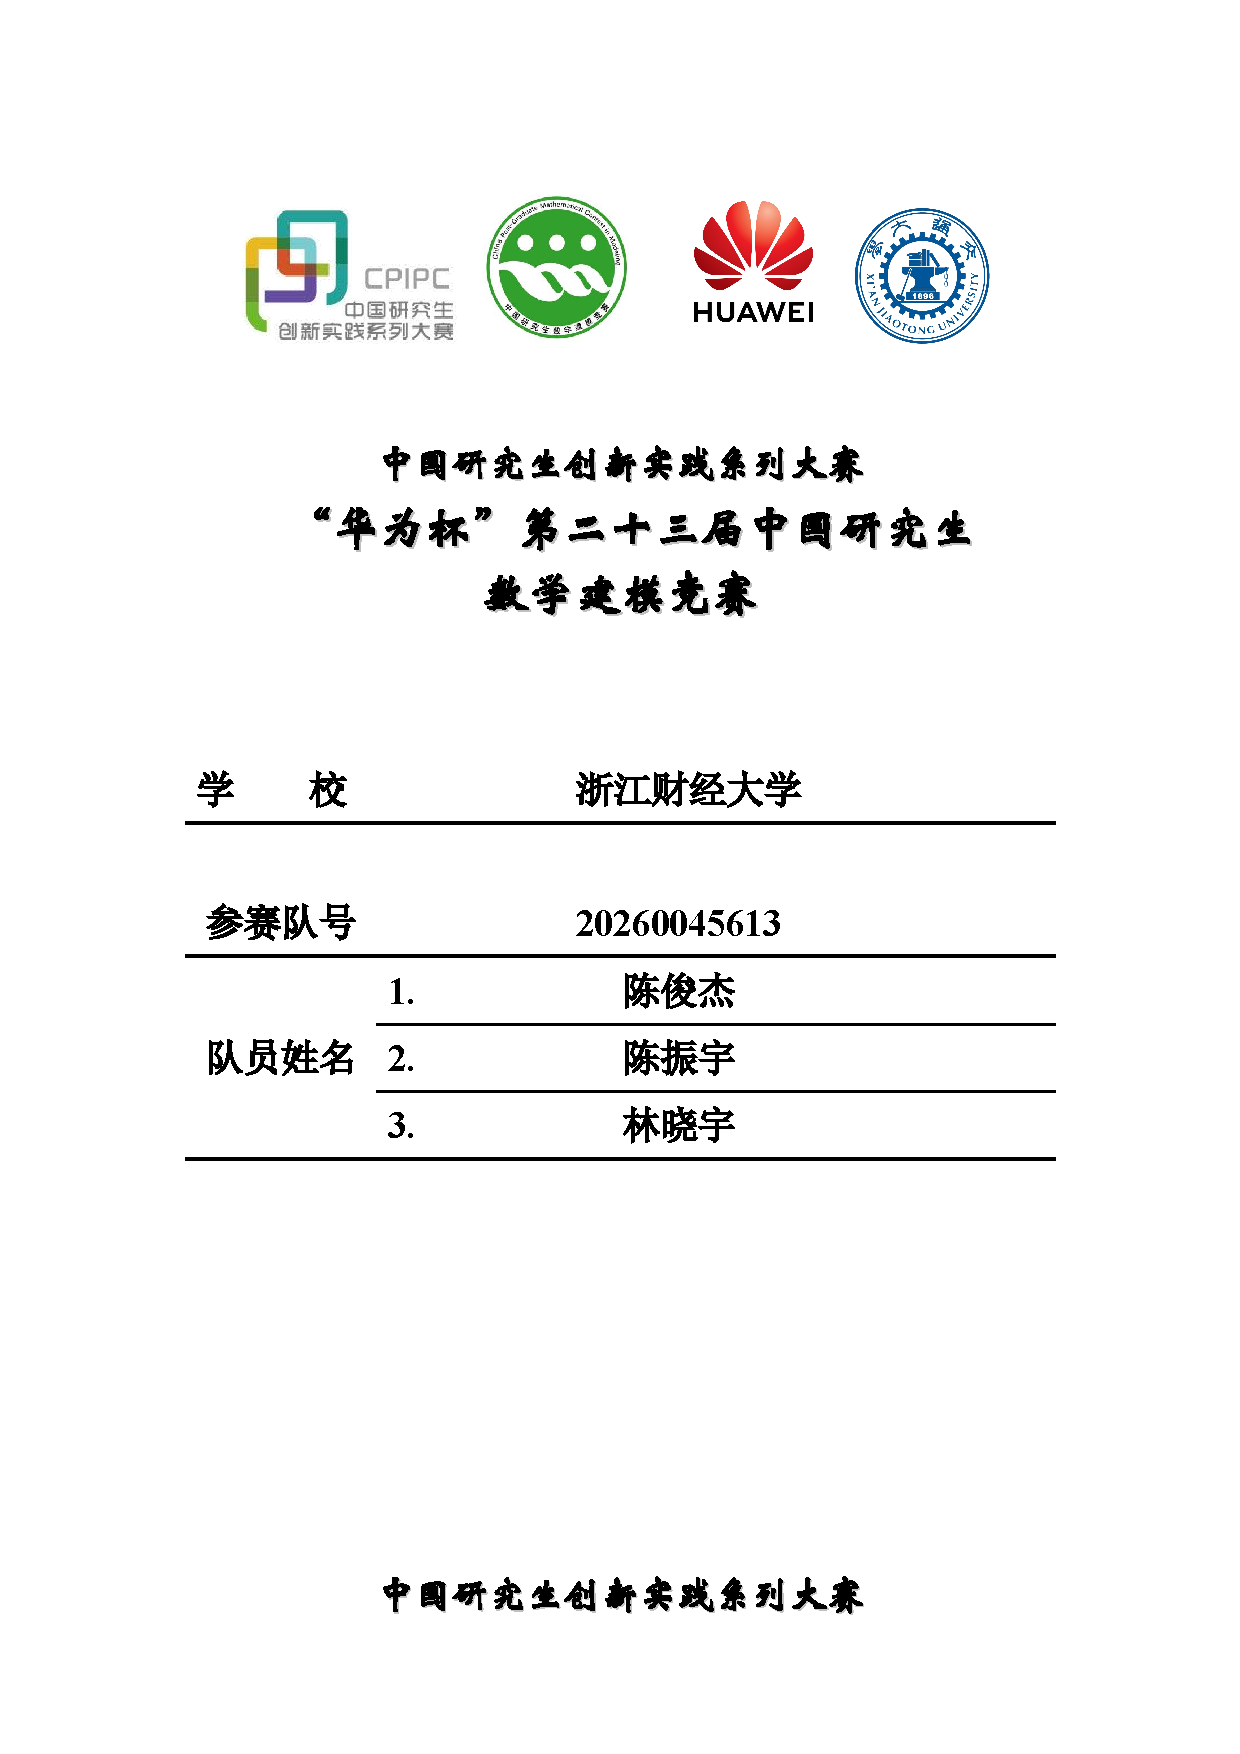
\includepdf[pages=-]{华为杯封面.pdf}
\newpage


%% -----------------------------------------------------------------------------
%% 模块 1：首页摘要对应段落（可直接合入 Abstract）
%% -----------------------------------------------------------------------------
\begin{center}
    {\zihao{-3} \heiti \textbf{摘\quad 要}}
\end{center}
\vspace{-0.2cm}
\hspace*{2\ccwd}大脑活动记录技术中，非侵入式脑电图（EEG）在脑机接口与精神疾病临床诊断中展现出重大应用前景。针对前额叶电极（Fz、F3、F4）极易受高幅眼动（EOG）等生理杂音干扰，且常规滤波极易破坏反映视物形状微弱神经特征的核心难题，本文围绕视觉认知两阶段加工机制，构建了集特征保护型残差自适应去噪、微观--介观--宏观跨尺度脑电计算模型以及多脑区协同认知网络于一体的完整理论与算法体系。

\textbf{针对问题一}，针对前额通道信噪比极低且设备自带滤波严重破坏视物特征的痛点，设计了\textbf{特征保护型残差双分量自适应校正与三次 B 样条拟合模型}。首先，通过 60 Hz 陷波与 0.1--30 Hz 零相位四阶双向带通实现保相滤波，结合硬件截幅、极差与物理跃变等多维工程准则进行坏试次客观筛查；其次，采用五折分层交叉验证框架，从同向低伪影试次中构建中位数基底模板并分离单试次残差，解耦提取垂直瞬目与水平扫视正交分量；引入基于稳健中位数绝对偏差（MAD）的软门控激活机制与带边界约束的岭回归模型估计耦合系数，并创新性提出\textbf{“训练均值保护（Training Mean Protection）”机制}，在滤除试次间剧烈波动的同时严格约束平均诱发波形的系统性偏离；最后，采用内部结点间隔 50 ms 的三次 B 样条平滑拟合 250--500 ms 认知窗内的正向诱发电位（P300）。实测数据表明：相对预处理基线，本模型使代理 MAE 点估计下降 \textbf{5.4\%--10.0\%}（受试者 A 项目一降幅达 \textbf{10.0\% [4.9\%, 13.8\%]}）；信噪比代理量平均提升 \textbf{0.03--0.48 dB}；视物形状左右差分幅度保留比达到 \textbf{0.813--0.952}，差分波形相关性均值高于 \textbf{0.99}；在半合成人工伪影注入闭环验证中，本模型在强污染下将归一化 RMSE 显著降低 \textbf{11.5\%}，兼具优异的去噪能力与高度的特征保真性。

\textbf{针对问题二}，针对视觉刺激如何跨尺度传导至头皮电极的机理阐释难题，构建了\textbf{图像驱动的三级兴奋--抑制（E/I）神经元群体计算模型}。首先，基于 COSFIRE 空间边缘组合思想提取左右三角形的几何轮廓特征，建立对偶镜像偏好输入；其次，采用 Wilson--Cowan 型非线性动力学方程刻画“LGN中继 $\to$ 早期视皮层 $\to$ 形状整合 $\to$ 前额响应”的级联演化，并以突触等效电流偶极子结合岭正则化优化求解前额头皮（Fz/F3/F4）的有效观测矩阵 $\hat{\mathbf{L}}$；进而通过固定参数消融与重拟合检验，定量揭示了左右三角产生的脑电波形差异本质上源于几何轮廓非对称性在皮层网络中的非线性传导以及跨半球投射偏侧化。最后，构建融合时域统计、峰潜伏期、偏侧化指数（LI）、机制模板投影系数及残差 RMS 的 \textbf{23 维机制增强特征向量}。在严格的五时间块独立留出测试中，方向差分指标 $S_\Delta$ 在两组数据中显著优于零差基线（受试者 B2 达 0.2562），跨受试者迁移判别平衡准确率最高达 \textbf{62.31\%}（AUC 为 \textbf{0.5807}），为空间视觉线索的神经机制解释与脑电特征表征提供了科学自洽的计算模型支撑。

\vspace{0.5cm}
\thispagestyle{empty} 
\newpage

\begingroup
  \pagestyle{empty}                   % 隐藏目录第二页（及后续页）的页码
  \let\oldthispagestyle\thispagestyle % 备份原命令
  \renewcommand{\thispagestyle}[1]{}  % 屏蔽目录内部强制设置的 plain 样式
  \tableofcontents                    % 生成目录
\endgroup
\thispagestyle{empty} 
\newpage



\pagenumbering{arabic} % 设置页码格式为阿拉伯数字（会自动重置为1）
\setcounter{page}{1}   % 明确设置起始页码为1（双重保险）


%% -----------------------------------------------------------------------------
%% 模块 2：问题重述中关于问题一的部分
%% -----------------------------------------------------------------------------
\section{问题重述}
\subsection{研究背景}
大脑是自然界中最复杂的器官之一，其活动可以通过多种神经影像方法进行记录和观测。在这些方法中，皮层脑电图（ECoG）和脑电图（EEG）分别代表了侵入性和非侵入性技术的典型。尽管侵入性技术具有信号分辨率高的优势，但其伴随的手术风险以及记录信号随时间逐渐退化的缺陷，限制了其广泛应用。相比之下，非侵入性脑电图技术因其安全性高、操作便捷等特点，在探索人类大脑活动方面展现出更为广阔的应用前景。

脑电图的应用范围涵盖从基础神经科学研究到临床医学的多个领域。脑电图驱动的计算模型作为连接基础神经科学研究与神经临床应用的核心桥梁，能够为科研人员与临床工作者提供可在虚拟环境中验证假说的高效平台，精准预测现实中难以直接实施的复杂实验与神经交互结果，其目标是生成可与真实实验数据进行对比的变量时间序列。当前，精神和神经系统疾病影响着越来越多的人群，带来了巨大的经济和人道主义负担。影响患者诊疗的主要障碍之一，是缺乏个体化的诊断、预后评估和治疗方案；另一个障碍则在于对精神性疾病机制——包括治疗方法起效的具体机制——普遍认知不足。根据个体可用数据调整模型参数，脑电图计算模型可实现个性化适配，为精准医疗提供可能。例如，深部脑刺激（DBS）是治疗晚期帕金森病的高效手段，但目前尚不完全清楚这种刺激如何精确抑制震颤等运动症状，而脑电图计算模型有望为此提供解释。

在脑电图的节律特征研究中，运动皮层产生的$\beta$节律在自主运动期间会受到抑制，这一现象称为运动相关$\beta$衰减（MRBD）；运动结束后，$\beta$振荡幅度会出现短暂回升，即运动后$\beta$反弹（PMBR），两者统称为$\beta$波段调制。研究表明，在精神分裂症患者中，PMBR显著减弱，且$\beta$反弹的幅度与患者当前症状的严重程度显著相关，凸显了其作为疾病生物标志物的临床价值。此外，阿尔茨海默症患者的脑电图计算模型分析显示，源于海马体的信号逐渐变得迟缓且微弱，这可能是该病的早期症状，为早期干预提供了可能。未来，理论上也可通过脑电图分析辅助精神分裂症、躁狂抑郁症等精神性疾病的诊断。

在脑机接口（BCI）领域，最具挑战性的课题之一是探索记录到的脑活动脑电图与人体模型、生物力学机制及认知加工之间的内在关联。脑电图通过检测神经元树突突触兴奋过程中电流流动所引发的脑电活动来工作，它不仅反映大脑皮层的电活动，也包含深部脑结构发出的信息。脑电图驱动的计算模型既可为BCI系统的脑活动解码与交互控制提供理论支撑与算法框架，也能在神经机制探索、神经性疾病临床研究中承担虚拟实验平台的功能，通过仿真模拟完成实验方案预演与科学假设的定量检验，大幅降低真实实验的试错成本与伦理风险。

从电生理学和网络层面研究大脑活动机理，通常采用不同空间尺度的脑电图信号计算模型。微观尺度模型以霍奇金-赫胥黎模型为代表，描述单个神经元或微电路的电活动特性；介观尺度模型如Wilson-Cowan神经质量模型，在神经集群或神经场层面建立平均场方程，描述兴奋性神经元群与抑制性神经元群之间的耦合关系；宏观尺度模型如藏本（Kuramoto）模型，通过引入序参数来描述大量弱耦合振子的同步行为，考虑脑网络中不同脑区之间的长程耦合作用及信号传输时间延迟。虽然对单神经元动作电位计算特性的研究已取得显著进展，但运动和感知通常源于大脑系统中皮层、丘脑和脊髓神经元群的集体行为，迄今为止尚无广泛接受的神经元群体集体活动的数学理论。我们的目标是通过建立脑电图计算模型明确脑电图实证数据与感知行为之间的联系。

认知是大脑的重要功能，大脑前额叶是主要的认知功能区，海马结构是主要的记忆功能区。视觉刺激从视网膜传入，经外侧膝状体核（LGN）投射至大脑皮层，最终在头皮被脑电图观测到。然而，观测目标与观测脑电图数据之间的联系难以确定：一方面，脑电图数据处理与解读存在诸多技术难题，观测信号中包含大量干扰（如眼动伪迹），而与视觉刺激相关联的信号较弱；另一方面，脑电图在头皮上采集信号，如何将二维头皮空间映射到三维大脑空间仍是未解难题。此外，现有的宏观模型如藏本模型虽能反映大量神经元同步后的脑电信号，但未考虑神经元的空间分布，而不同视物在大脑皮层产生的视觉刺激响应神经元分布存在差异，进而导致观测到的脑电图信号也有差异。如何将微观的神经元模型与宏观观测脑电图结合形成脑神经计算模型，是一个具有挑战性的课题。

综上所述，建立脑电图计算模型，将微观神经元模型与宏观观测脑电图相结合，揭示视觉刺激与脑电信号之间的映射关系，对于推动脑机接口技术发展、实现精神性疾病的早期诊断具有重要的科学意义和应用价值。基于此，本文围绕服务于脑机接口与精神性疾病诊断的脑电图计算模型展开研究。

\subsection{问题重述}
基于上述背景，本论文针对"服务于脑机接口与精神性疾病诊断的脑电图计算模型"展开研究。该问题以脑电图（EEG）为研究对象，旨在通过建立脑电图计算模型，揭示视觉刺激与脑电信号之间的内在关联机制，为脑机接口系统的脑活动解码和精神性疾病的辅助诊断提供理论支撑与算法框架。具体而言，本题需要解决以下三个子问题：

\noindent\textbf{问题1：脑电图信号预处理与视觉响应提取。}

针对实验项目1（目标位置已知，等待目标出现）和实验项目2（目标位置未知，仅知道目标形状）两种实验范式下的脑电图数据，设计特定的降噪方法，在保留视物形状相关脑电图特征的前提下，有效去除运动、眨眼等伪影干扰；提取不同观测点位（F3、Fz、F4）的有效视觉响应，并拟合相应曲线。该问题的核心在于如何在去噪与信号特征保留之间取得平衡——现有的多种去干扰方法在去除伪影的同时也破坏了反映视物的脑电图特征，因此需要设计特定的降噪策略，避免直接使用题目中机器自带滤波器处理后的数据（通道4-6），而是基于原始数据（通道1-3）进行自主处理。

\noindent\textbf{问题2：脑电图计算模型建立与视觉刺激区分机制解释。}

建立描述从外侧膝状体核（LGN）到大脑皮层再到头皮观测的脑电图信号形成机理的计算模型；利用所建立的模型解释左右三角形视觉刺激产生脑电信号差异的形成机制；并给出能够有效区分左右三角形视觉刺激响应的特征表示。该问题需要结合神经生理学证据——神经生理学研究表明，人脸等物体的识别是通过检测特定空间方式排列的某些特征来实现的，颞下皮层神经元对满足"轮廓包裹双眼、双眼位于嘴部上方"结构的刺激才会产生强响应——从神经元群体活动的角度阐释视觉刺激的脑电响应差异，进而建立视觉刺激物形状与大脑皮层响应神经元分布之间的联系，以及脑电图观测与大脑皮层响应神经元之间的联系。

\noindent\textbf{问题3：认知模型建立与验证。}

截取与视觉认知相关联的信号（该信号的终点可能是应答响应之前的大约100ms），借助问题二所建立的脑电信号形成机制，同时考虑信号可能同时来源于海马体和LGN等脑区，建立认知过程的宏观计算模型；并利用题目所提供的四组实验脑电图数据(VisualCogA\_Task-1.mat、VisualCogA\_Task-2.mat、VisualCogB\_Task-1.mat、VisualCogB\_Task-2.mat)验证该模型。需要注意的是，被试的应答行为不一定正确，也可能包括没有及时应答的情况，模型需对此进行合理处理。本题的实验数据采样率为256Hz，包含十个数据记录通道，涵盖原始数据、视觉提示、目标应答和时间戳等信息。

本文针对上述三个子问题依次开展建模研究：首先对脑电图原始数据进行预处理和降噪，提取有效视觉响应并拟合曲线；其次建立脑电图计算模型，解释视觉刺激差异导致脑电信号差异的机理并提取区分特征；最后建立认知宏观模型并利用实验数据进行验证。通过上述研究，给出可行的解决方案与结论。
\newpage


%% -----------------------------------------------------------------------------
%% 模块 3：问题分析中关于问题一的递进剖析
%% -----------------------------------------------------------------------------
\section{问题分析}

\subsection{问题一的分析}

问题一的核心任务是从两个视觉认知项目的原始脑电中提取有效视觉响应，并分别拟合 Fz、F3、F4 三个观测点的响应曲线。分析既要减弱干扰，也要检查处理过程是否改变了左右视觉提示所对应的波形特征。

\noindent\textbf{难点一：视觉响应较弱，伪影与目标信号相互混合。}

前额区脑电同时包含视觉任务相关活动、眼动、眨眼、运动及缓慢漂移等成分。这些干扰可能出现在视觉提示后的同一时段，仅依据幅度或频率难以将其与有效响应分开。两个实验项目的任务条件不同，响应形态也可能不同，因此还需分别分析，避免用总体平均波形掩盖项目差异。

\noindent\textbf{针对难点一：建立以视觉提示事件为基准的分项目处理流程。}

首先从原始 Fz、F3、F4 通道提取提示事件，对连续信号进行预处理，并通过固定的质量规则识别严重异常试次；然后在训练试次中估计响应参考和伪影校正参数，将确定的处理规则用于留出试次。处理后按项目、提示方向和通道计算事件相关平均波形，重点观察提示后 \(250\sim500\,\mathrm{ms}\) 的正向活动及三个电极之间的空间差异。

\noindent\textbf{难点二：降低波形波动与保留视觉特征需要同时评价。}

平滑或伪影校正可以使试次间波形更加接近，却也可能改变左右条件差异、正向峰值及其潜伏期。题目没有提供同步眼电或独立的无噪声脑电，设备处理后的 Decon 通道也不能充当干净真值。因此，单一误差指标不足以判断视觉信息是否得到保留。此外，三个电极均位于额区，不能仅凭这些记录认定观察到了中央--顶区的典型 P300。

\noindent\textbf{针对难点二：联合评价去噪效果、条件差异与曲线拟合质量。}

在相同试次上比较处理前后的波形波动、刺激前基线、左右条件差异以及特征时窗内的峰值和面积，并用训练试次构造的参考及人工污染恢复实验检验校正方法。随后对各条件平均响应进行曲线拟合，报告拟合残差和峰值位置。由此分别回答干扰是否减弱、观测到的响应形态如何变化，以及现有数据能够在何种程度上支持视觉特征保留的判断。

\subsection{问题二的分析}

问题二要求说明左右三角形视觉刺激如何经过视觉通路形成可观测的脑电差异，并给出区分两类刺激的特征表示。该问题同时涉及形状信息的编码、神经群体活动的形成和头皮电位的观测。

\noindent\textbf{难点一：图像形状与头皮脑电处于不同层次，内部来源无法直接观测。}

三角形的左右朝向属于图像空间结构，而 Fz、F3、F4 记录的是多个内部活动源叠加后的头皮电位。仅有三个额区通道时，即使模型能够拟合实测波形，也难以唯一确定每个内部状态对应的真实脑区。因此，需要构造各环节含义明确、能够生成预测波形的候选形成模型。

\noindent\textbf{针对难点一：按视觉输入、中继、群体动力学和头皮观测建立模型链。}

首先提取左右三角形的边缘及空间组合特征，形成具有方向差异的视觉输入；再设置 LGN 中继环节，将输入传递至具有形状选择性的皮层兴奋--抑制群体。由群体活动构造等效突触源，并通过同一观测映射生成三个额区通道的预测脑电。左右条件共享动力学和观测参数，使模型差异由刺激输入产生。最后比较留出试次的共同响应与左右差异波，并通过移除模型环节的实验检查各环节对预测的影响。

\noindent\textbf{难点二：波形拟合能力与未知方向的单试次区分能力并不相同。}

模型可能较好地重现两类刺激共有的平均波形，却无法稳定预测它们之间较弱的差异。第一问的部分校正过程利用了已知提示方向；若直接将此类输出用于未知方向判别，就会使判别特征预先包含待预测的信息。相邻试次还可能受到共同的慢变化影响，普通随机划分难以充分检验时间稳定性。

\noindent\textbf{针对难点二：将形成机制检验与方向判别分别验证。}

从原始三通道记录重新构建独立时间块，在训练块内完成预处理参数估计、模型选择和特征标准化。分别提取时域幅度、峰值潜伏期、空间差异及机制模型投影特征，再对留出时间块进行未知方向预测。通过简单特征基线、块内置换和多特征比较检验判别结果，区分模型内部的形状响应、实测差异预测与单试次识别能力。

\subsection{问题三的分析}

问题三需要把视觉提示、目标出现和应答前的脑电活动联系起来，建立认知过程的宏观模型。相较于前两问，本问的观测时间更长，还需要处理应答错误或未及时应答的可能情形。

\noindent\textbf{难点一：事件标记的含义及应答前分析窗口需要谨慎确定。}

提示、候选目标和点击标记并非都具有相同的确定性。项目二记录了独立点击，项目一的部分应答时刻只能由标记变化推定。若将应答后的活动纳入认知模型，可能混入动作相关信号；若将没有明确点击标记的试次直接判为超时，又会赋予数据中并不存在的行为标签。

\noindent\textbf{针对难点一：区分事件证据并制定统一的截窗规则。}

先核对四组记录中的提示、候选目标和应答标记，将独立点击、应答代理与应答不可观测的试次分别标识。有可用应答时，将脑电分析终点限制在应答前约 \(100\,\mathrm{ms}\)；无明确应答时，采用预先规定的有限观察窗，并检查记录边界和试次质量。长时间序列使用符合时间顺序的信号处理方式，减少未来观测对较早认知状态估计的影响。

\noindent\textbf{难点二：记忆和认知活动可能表现为缓慢变化，难与一般背景趋势区分。}

题目要求考虑海马体等潜在来源，但额区头皮脑电不能直接定位深部结构。提示后的缓慢活动也可能来自背景漂移、任务准备或其他过程。若模型只在训练数据中得到较好拟合，尚不足以说明记忆环节对实测脑电提供了额外解释。

\noindent\textbf{针对难点二：建立功能性认知状态，并与简单慢趋势模型比较。}

继承第二问的形状编码和视觉形成结构，分别描述提示保持、目标触发提取与认知整合过程，再将这些状态映射到头皮观测波形。以留出时间块上的预测误差为依据，比较含记忆状态的模型与普通慢趋势模型在目标前后各阶段的表现，并分析观察窗和参数变化对结论的影响。模型中的记忆变量表示功能过程，其生理来源仍需独立证据检验。

\noindent\textbf{难点三：缺少可确认的真实正误与实验超时标签。}

现有数据没有提供完整的逐试次目标布局、正确目标映射和实验规定的超时阈值。点击方向不能直接转换为答题正误，缺失点击也不能直接转换为实验超时。因此，真实脑电验证与正确、错误、未决行为的研究需要采用不同的评价口径。

\noindent\textbf{针对难点三：用决策仿真分析模型行为，并与实测观测分开报告。}

将认知状态作为决策过程的输入，在给定的模拟目标布局和观察期限下生成正确、错误及未决三类结局，考察记忆保持、证据增益和噪声变化对模拟结果的影响。真实数据用于检验脑电波形及可确认的点击时间；模拟结局用于说明模型能够产生何种行为，不将其作为实测正确率或真实超时率。


%% -----------------------------------------------------------------------------
%% 模块 4：模型假设与符号说明表
%% -----------------------------------------------------------------------------
\newpage
\section{模型假设与符号说明}

\subsection{模型假设}

为突出问题本质并保证模型可求解，在不改变实验含义的前提下作如下基本假设：

假设一：同一受试者、同一实验项目和同一刺激方向下，重复试次具有稳定的条件诱发响应，其余与刺激无关的随机扰动经多次平均后趋于零。

假设二：原始脑电可视为刺激相关活动、背景脑电与生理伪迹的叠加；有限幅度的伪迹校正能够减弱干扰，且不系统改变条件平均响应的主要形态。

假设三：左、右三角形除朝向外具有相同的视觉属性；同一记录内两类刺激共享 LGN 中继、皮层群体动力学及头皮观测结构，其差异主要由形状输入与偏侧化投射产生。

假设四：视觉提示、目标出现与应答过程在时间上可分段描述；模型状态表示相应脑区的功能性群体活动，事件代理仅用于确定分析时窗，不直接等同于真实正误或超时标签。


\subsection{符号说明}

\begingroup
\captionsetup{labelsep=space}
\renewcommand{\arraystretch}{1.24}
\setlength{\tabcolsep}{4pt}
\begin{longtable}{@{}>{\centering\arraybackslash}p{0.22\textwidth}>{\centering\arraybackslash}p{0.60\textwidth}>{\centering\arraybackslash}p{0.12\textwidth}@{}}
\caption{本文的符号说明}\label{tab:all_symbols}\\
\toprule
符号 & 说明 & 单位 \\
\midrule
\endfirsthead
\multicolumn{3}{c}{\small 表~\thetable\ 本文的符号说明（续）}\\
\toprule
符号 & 说明 & 单位 \\
\midrule
\endhead
\bottomrule
\endfoot
\(r\) & 数据记录编号，取值为 A1、A2、B1 或 B2 & 无 \\
\(i\) & 单组脑电记录中的试次编号 & 无 \\
\(c\) & 脑电观测通道编号，取值为 Fz、F3 或 F4 & 无 \\
\(f_s\) & 脑电采样频率，\(f_s=256\) & Hz \\
\(t\) & 相对于视觉提示起点的时间 & s \\
\(d_i\) & 第 \(i\) 次提示的方向，左、右分别记为 \(-1,+1\) & 无 \\
\(x_{r,i,c}(t)\) & 第 \(r\) 组记录中第 \(i\) 个试次在通道 \(c\) 上的原始脑电 & 原始单位 \\
\(\tilde{x}_{r,i,c}(t)\) & 特征保护型方法校正后的单试次脑电波形 & 原始单位 \\
\(\bar{x}_{r,d,c}(t)\) & 记录 \(r\)、方向 \(d\)、通道 \(c\) 的条件平均响应 & 原始单位 \\
\(I_d\) & 朝向为 \(d\) 的标准化三角形图像输入 & 无 \\
\(g(t)\) & LGN 的中继状态 & 模型单位 \\
\(E_s(t)\) & 第 \(s\) 级皮层兴奋性群体状态 & 模型单位 \\
\(I_s(t)\) & 第 \(s\) 级皮层抑制性群体状态 & 模型单位 \\
\(\boldsymbol{\phi}_i\) & 用于提示方向判别的单试次机制增强特征向量 & 混合 \\
\(z(t)\) & 行为仿真中的累积决策变量 & 无 \\
\end{longtable}
\endgroup


%% -----------------------------------------------------------------------------
%% 模块 5：模型的建立与求解（核心篇幅）
%% -----------------------------------------------------------------------------
\newpage
\section{模型建立与求解}
\subsection{问题一模型的建立与求解}
\renewcommand{\theequation}{1-\arabic{equation}}
\renewcommand{\theHequation}{q1.\arabic{equation}}
\setcounter{equation}{0}

为解决原始额区脑电中视觉响应微弱、瞬目与扫视伪影幅值较大且常规强滤波容易改变条件波形的问题，本文建立特征保护型残差双分量自适应校正模型。模型以原始 $F_z$、$F_3$、$F_4$ 三通道及视觉提示事件为输入，依次完成连续信号保相滤波、坏试次筛查、折外代理模板构建、双分量伪影估计、保守校正、条件事件相关电位提取与三次 B 样条拟合，最终输出两个实验项目在三个观测点的左右刺激响应曲线。设备自带处理通道仅用于可视化对照，不参与建模与评价。

\subsubsection{数据预处理}

\paragraph{（1）数据通道与事件审计}

题目给出受试者 A、B 在项目一和项目二下的四组数据，采样率均为 $f_s=256\,\mathrm{Hz}$。本文只读取原始通道 $F_z$、$F_3$、$F_4$ 和视觉提示通道 \texttt{VisCue}；其中 \texttt{VisCue} 从 $0$ 跳变为 $-1$ 或 $+1$ 的时刻分别记为左、右三角形提示起点。以提示起点 $t_i$ 为零时刻，截取区间 $[-250,796.875]~\mathrm{ms}$，并将 $250$--$500~\mathrm{ms}$ 作为题目给定的主要视觉响应分析窗。由于数据未提供可信的物理标定信息，全文幅值均记为“原始电位单位”，不擅自换算为 $\mu\mathrm{V}$。

设备自带的 \texttt{FzDecon}、\texttt{F3Decon}、\texttt{F4Decon} 已改变原始波形的低频趋势，不能作为无噪声真值。图~\ref{fig:q1_preprocess_waveform} 给出同一试次三通道原始记录、设备处理结果与本文预处理及校正结果的对照。可以看出，设备处理曲线与原始曲线存在明显形态差异，因此后续方法完全从原始三通道重新计算。

\begin{figure}[H]
    \centering
    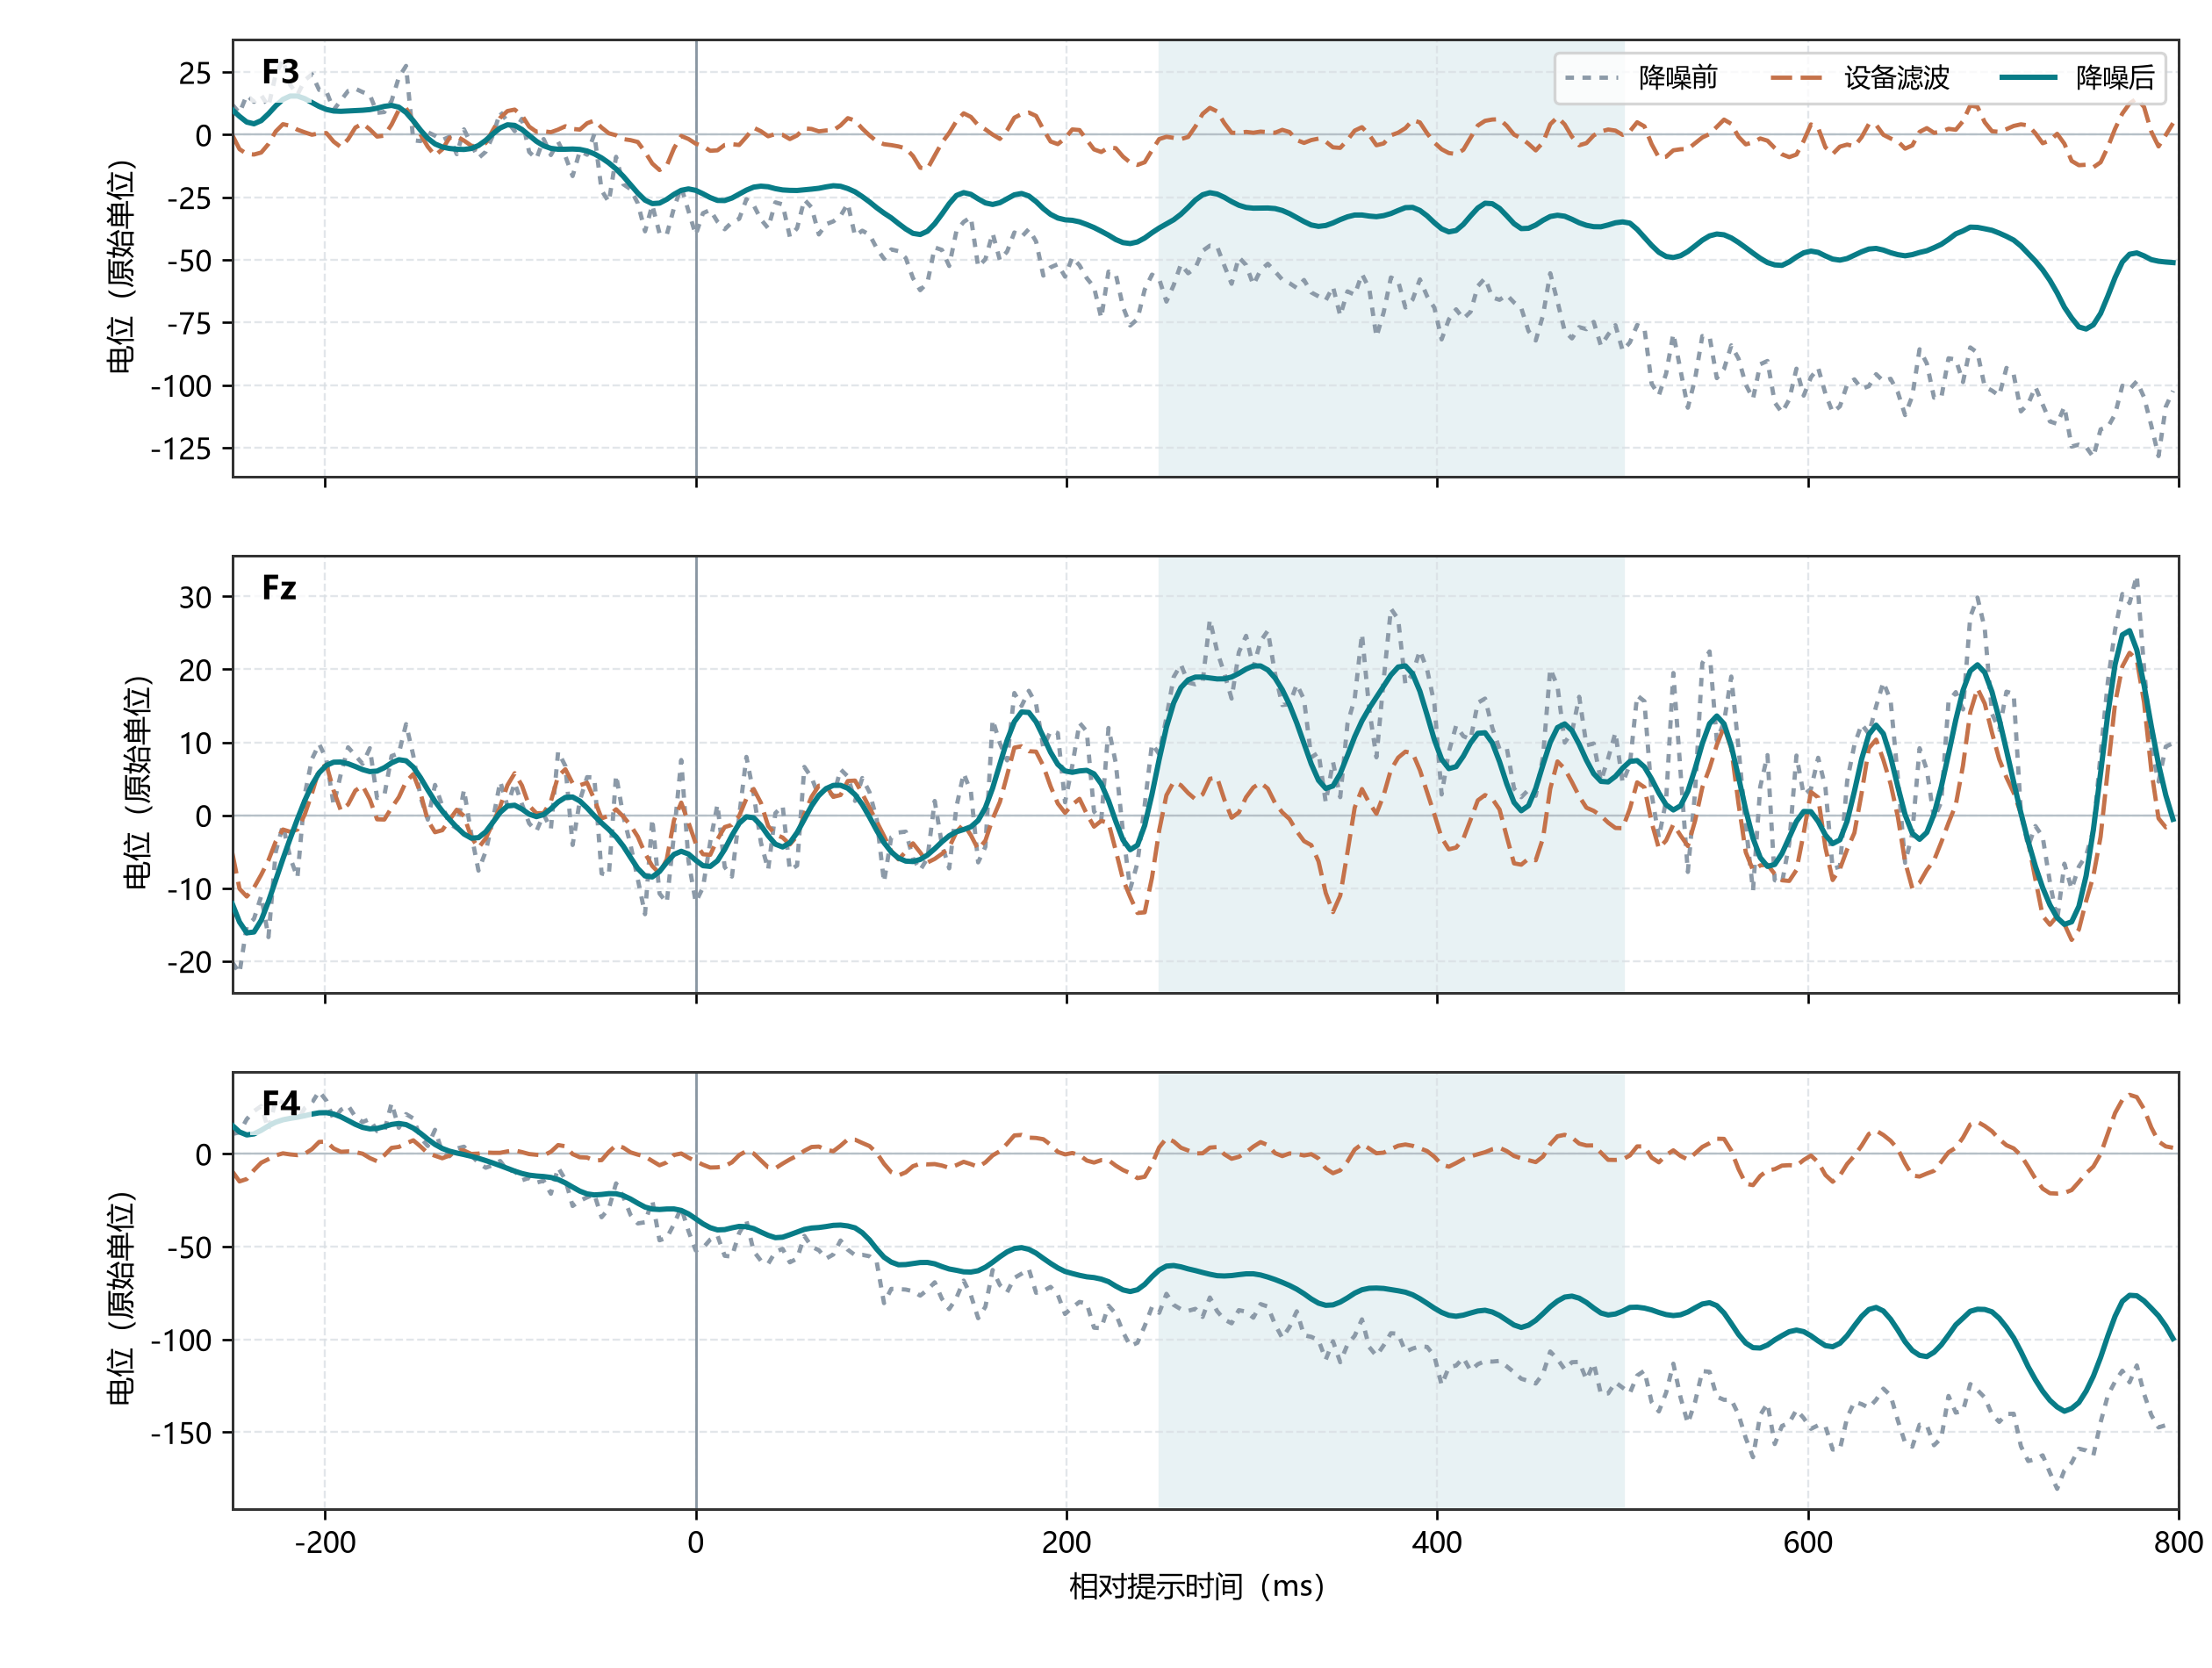
\includegraphics[width=0.94\textwidth]{q1_waveform.png}
    \caption{同一试次三通道原始记录、设备处理与本文处理结果对比}
    \label{fig:q1_preprocess_waveform}
\end{figure}

\paragraph{（2）连续信号保相滤波与基线校正}

首先对连续信号施加中心频率为 $60\,\mathrm{Hz}$、品质因数 $Q=30$ 的二阶 IIR 陷波器，以削弱工频干扰；随后采用 $0.1$--$30\,\mathrm{Hz}$ 四阶 Butterworth 带通滤波器。两类滤波均以前后双向方式执行，使总体相位响应为零，从而避免因因果滤波时延改变峰潜伏期。记陷波与带通算子分别为 $\mathcal{F}_{\mathrm{notch}}$ 和 $\mathcal{F}_{\mathrm{bp}}$，则滤波信号为

\begin{equation}
    x^{(f)}_c(t)=\mathcal{F}_{\mathrm{bp}}\!\left(\mathcal{F}_{\mathrm{notch}}\!\left(x^{(0)}_c(t)\right)\right),
    \quad c\in\{F_z,F_3,F_4\}.
    \label{eq:q1_filter}
\end{equation}

完成事件分段后，以刺激前 $[-250,0)~\mathrm{ms}$ 的中位数进行稳健基线校正：

\begin{equation}
    x_{i,c}(t)=x^{(f)}_{i,c}(t)-
    \mathop{\mathrm{median}}_{u\in[-250,0)}x^{(f)}_{i,c}(u),
    \label{eq:q1_baseline}
\end{equation}

其中，$i$ 为试次编号，$c$ 为通道，$t$ 为相对提示时间。选择 $0.1\,\mathrm{Hz}$ 低截止频率的目的是保留项目二中较慢的条件平均变化；若直接提高高通截止频率，虽然可减小漂移，但也可能人为改变宽缓响应的幅值与潜伏期。

\paragraph{（3）严重坏试次筛查}

为避免硬件截幅、极端振幅和非生理跳变支配均值，本文在任何模板估计前固定三项工程阈值。设试次 $i$ 的跨通道饱和点数、最大峰峰值和最大相邻点跳变分别为 $S_i$、$P_i$ 和 $J_i$，则坏试次指示量定义为

\begin{equation}
    b_i=\mathbf{1}\!\left(S_i\ge 15\ \lor\ P_i>1800\ \lor\ J_i>600\right),
    \label{eq:q1_badtrial}
\end{equation}

其中，$S_i=\sum_{c,t}\mathbf{1}(|x^{(0)}_{i,c}(t)|\ge999)$，$P_i=\max_c\{\max_t x_{i,c}(t)-\min_t x_{i,c}(t)\}$，$J_i=\max_{c,t}|x_{i,c}(t)-x_{i,c}(t-1)|$。这些阈值由当前数据量纲下的异常分布与硬件截幅特征确定，只用于剔除不可恢复的极端记录，不把一般的高幅试次预先删除。筛查结果如表~\ref{tab:q1_trial_audit} 所示，四组数据共保留 $371$ 个试次。

\begin{table}[H]
    \centering
    \caption{四组实验数据的事件与有效试次对账}
    \label{tab:q1_trial_audit}
    \begin{tabular}{lccccc}
        \toprule
        \textbf{数据组} & \textbf{提示事件数} & \textbf{边界剔除} & \textbf{质量剔除} & \textbf{有效试次} & \textbf{左/右试次} \\
        \midrule
        受试者 A 项目一 & 100 & 0 & 10 & 90 & 47/43 \\
        受试者 A 项目二 & 100 & 0 & 5  & 95 & 53/42 \\
        受试者 B 项目一 & 100 & 0 & 6  & 94 & 46/48 \\
        受试者 B 项目二 & 100 & 0 & 8  & 92 & 45/47 \\
        \bottomrule
    \end{tabular}
\end{table}

\subsubsection{评价指标}

问题一没有同步眼电或独立无噪声脑电，故设备处理波形与训练模板均不能视为真实标签。为同时评价去噪、条件差异保留与曲线拟合，本文采用代理参考误差、信噪比代理量、左右差异保留率、半合成恢复误差和样条拟合误差五类互补指标，而不将其合成为单一分数。

\paragraph{（1）代理参考误差与信噪比代理量}

在第 $k$ 个外折中，仅用训练试次构造方向 $d\in\{-1,+1\}$ 的代理模板 $T^{(k)}_{d,c}(t)$。测试集方向平均响应记为 $\bar{x}^{(k)}_{d,c}(t)$，则 $250$--$500~\mathrm{ms}$ 窗内的代理平均绝对误差为

\begin{equation}
    \mathrm{MAE}_{\mathrm{proxy}}=
    \frac{1}{|\mathcal{W}|}\sum_{t\in\mathcal{W}}
    \left|\bar{x}^{(k)}_{d,c}(t)-T^{(k)}_{d,c}(t)\right|,
    \quad \mathcal{W}=[250,500]~\mathrm{ms}.
    \label{eq:q1_mae}
\end{equation}

该指标越小，说明测试条件平均曲线越接近训练折内的低伪影参考，但不能据此断言更接近真实神经信号。进一步以 $0$--$500~\mathrm{ms}$ 内 ERP 功率与单试次相对 ERP 的残差功率之比定义信噪比代理量：

\begin{equation}
    \mathrm{SNR}_{\mathrm{proxy}}=10\log_{10}
    \frac{\frac{1}{|\mathcal{W}_0|}\sum_{t\in\mathcal{W}_0}\bar{x}_{d,c}^{,2}(t)}
    {\frac{1}{N_d|\mathcal{W}_0|}\sum_{i:y_i=d}\sum_{t\in\mathcal{W}_0}
    \left[x_{i,c}(t)-\bar{x}_{d,c}(t)\right]^2},
    \quad \mathcal{W}_0=[0,500]~\mathrm{ms}.
    \label{eq:q1_snr}
\end{equation}

残差中仍含真实的试次间变异，因此该指标只反映条件平均响应相对试次波动的突出程度。

\paragraph{（2）视觉条件差异保留指标}

令 $\Delta_c^{\mathrm{pre}}(t)$ 与 $\Delta_c^{\mathrm{V7}}(t)$ 分别表示预处理后和校正后左减右 ERP 差分，则定义差分幅度保留率与形状相关系数为

\begin{equation}
    R_{\Delta,c}=
    \frac{\left\|\Delta_c^{\mathrm{V7}}\right\|_2}
    {\left\|\Delta_c^{\mathrm{pre}}\right\|_2},
    \qquad
    \rho_{\Delta,c}=\operatorname{corr}
    \left(\Delta_c^{\mathrm{V7}},\Delta_c^{\mathrm{pre}}\right),
    \label{eq:q1_retention}
\end{equation}

其中范数和相关均在 $250$--$500~\mathrm{ms}$ 计算。$R_{\Delta,c}$ 接近 $1$ 且 $\rho_{\Delta,c}$ 较高，仅表示处理前后的条件差异较接近；若原始条件差异含方向相关眼动，该指标同样会保留该成分，因而不是视觉神经特异性的直接证据。

\paragraph{（3）已知目标恢复误差与曲线拟合误差}

在半合成检验中，将人工伪影加入预处理实测背景，以污染前波形 $x^{\ast}$ 为可计算目标。归一化恢复误差定义为

\begin{equation}
    \mathrm{NRMSE}=
    \frac{\sqrt{\frac{1}{NCT}\sum_{i,c,t}\left(\hat{x}_{i,c}(t)-x^{\ast}_{i,c}(t)\right)^2}}
    {\sqrt{\frac{1}{NCT}\sum_{i,c,t}\left(x^{\ast}_{i,c}(t)\right)^2}},
    \label{eq:q1_nrmse}
\end{equation}

该指标可以检验对“额外注入污染”的恢复能力，但污染前实测背景仍可能含原有伪影。对于最终 ERP 的三次 B 样条拟合，另以同一样本上的残差均方根误差 $\mathrm{RMSE}_{\mathrm{fit}}$ 描述平滑拟合程度，它不是独立预测误差。

\paragraph{（4）不确定性估计与指标解释}

对左右方向分别进行配对试次 Bootstrap 重采样，预处理与 V7 共用同一批索引；组均值指标使用 $800$ 次重采样并报告 $95\%$ 区间。图~\ref{fig:q1_metric_dashboard} 汇总了代理 MAE 降幅、SNR 代理增量和左右差异保留率。可见四组代理 MAE 降幅点估计均为正，区间为 $5.4\%$--$10.0\%$；SNR 代理增量仅为 $0.027$--$0.481~\mathrm{dB}$，且四组区间均跨过零点；左右差异保留率点估计为 $0.813$--$0.952$。因此，评价证据支持“校正后更接近训练代理参考且未大幅压缩处理前条件差异”，但不支持“真实神经信噪比已稳定提高”这一更强结论。

\begin{figure}[H]
    \centering
    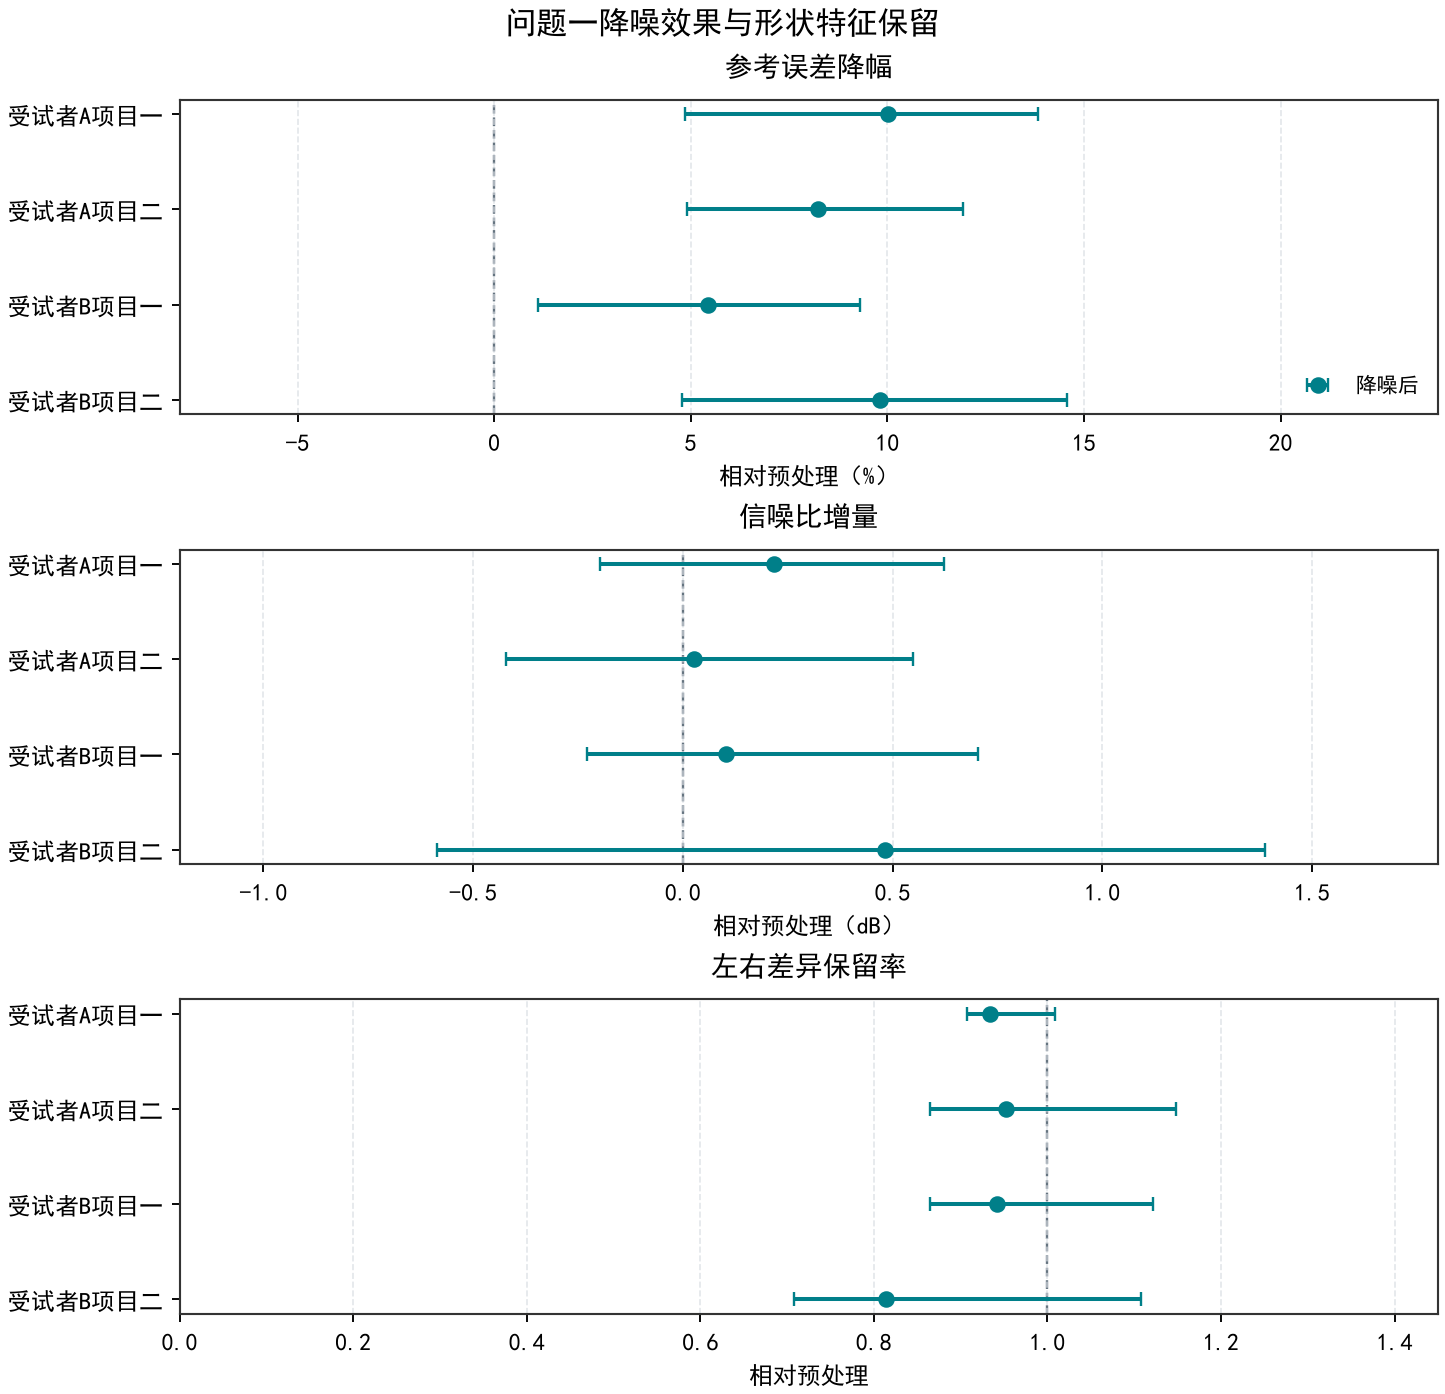
\includegraphics[width=0.86\textwidth]{q1_metrics.png}
    \caption{四组数据的去噪代理指标与左右条件差异保留结果}
    \label{fig:q1_metric_dashboard}
\end{figure}

\begin{table}[H]
    \centering
    \caption{问题一核心评价结果及 $95\%$ Bootstrap 区间}
    \label{tab:q1_core_metrics}
    \resizebox{\textwidth}{!}{%
    \begin{tabular}{lcccc}
        \toprule
        \textbf{数据组} & \textbf{有效试次} & \textbf{代理 MAE 降幅/\%} & \textbf{SNR 代理增量/dB} & \textbf{左右差异保留率} \\
        \midrule
        受试者 A 项目一 & 90 & 10.0 [4.9, 13.8] & 0.217 [$-0.197$, 0.623] & 0.934 [0.908, 1.009] \\
        受试者 A 项目二 & 95 & 8.2 [4.9, 11.9]  & 0.027 [$-0.422$, 0.549] & 0.952 [0.865, 1.148] \\
        受试者 B 项目一 & 94 & 5.4 [1.1, 9.3]   & 0.103 [$-0.228$, 0.702] & 0.942 [0.865, 1.121] \\
        受试者 B 项目二 & 92 & 9.8 [4.8, 14.6]  & 0.481 [$-0.585$, 1.388] & 0.813 [0.708, 1.107] \\
        \bottomrule
    \end{tabular}%
    }
\end{table}

\subsubsection{问题求解与模型建立}

\paragraph{（1）五折外层划分与训练代理模板}

将每组有效试次按左右方向分层划分为五折，随机种子固定为 $42$。对第 $k$ 折，测试试次不参与模板、残差尺度或候选策略的估计。首先在训练集内按稳健伪影得分从低到高排序，分别选取左右方向中较低的 $50\%$ 试次，并计算逐时间点中位数：

\begin{equation}
    T^{(k)}_{d,c}(t)=
    \mathop{\mathrm{median}}_{i\in\Omega^{(k)}_{d,\mathrm{low}}}
    x_{i,c}(t),
    \qquad d\in\{-1,+1\}.
    \label{eq:q1_template}
\end{equation}

该模板的作用是从单试次中分离相对于同方向条件平均的异常波动，而不是充当无噪声真值。单试次残差写为 $r_{i,c}(t)=x_{i,c}(t)-T^{(k)}_{d,c}(t)$。

\paragraph{（2）垂直--水平双分量与软门控}

前额区瞬目通常在三个导联上表现为较强的同相变化，水平扫视则更容易在 $F_3$ 与 $F_4$ 形成反相差异。基于这一几何结构，从残差构造垂直与水平候选参考：

\begin{equation}
    v_i(t)=\mathop{\mathrm{median}}_{c\in\{F_z,F_3,F_4\}}r_{i,c}(t),
    \qquad
    h_i(t)=\frac{r_{i,F_4}(t)-r_{i,F_3}(t)}{2}.
    \label{eq:q1_components}
\end{equation}

分别用约 $160~\mathrm{ms}$ 和 $120~\mathrm{ms}$ 的 Savitzky--Golay 窗对 $v_i$、$h_i$ 平滑。设训练折估计的逐点 MAD 尺度为 $s_q(t)$，门控阈值和过渡宽度为 $\eta_q$、$w$，则软门控分量统一表示为

\begin{equation}
    a_q(t)=\tilde q(t)\cdot
    \operatorname{clip}\!\left(
    \frac{|\tilde q(t)|/(s_q(t)+\varepsilon)-\eta_q}{w},0,1
    \right),
    \qquad q\in\{v,h\}.
    \label{eq:q1_gate}
\end{equation}

软门控使低于训练残差尺度的波动基本保持不变，而对超过阈值的缓慢同相或反相成分逐渐增加校正强度，从而减小硬阈值引起的波形突变。

\paragraph{（3）带边界约束的岭回归校正}

将两个门控分量组成设计矩阵 $\mathbf A_i=[a_v,a_h]$。对每个通道分别求解

\begin{equation}
    \hat{\boldsymbol\beta}_{i,c}=
    \arg\min_{\boldsymbol\beta}
    \left\|\mathbf r_{i,c}-\mathbf A_i\boldsymbol\beta\right\|_2^2
    +\lambda\left\|\boldsymbol\beta\right\|_2^2,
    \label{eq:q1_ridge}
\end{equation}

其中 $\lambda=0.05$。垂直系数限制在 $[0,1.8]$，水平系数限制在 $[-1.5,1.5]$；由于 $F_z$ 位于中线，其水平系数进一步限制在 $[-0.3,0.3]$。全量候选改动量为

\begin{equation}
    \delta_{i,c}(t)=\mathbf A_i(t)\hat{\boldsymbol\beta}_{i,c},
    \qquad x^{\mathrm{cand}}_{i,c}(t)=x_{i,c}(t)-\delta_{i,c}(t).
    \label{eq:q1_candidate}
\end{equation}

岭正则与系数边界共同限制了共线分量的过度扣除；但由于只有三个额区通道，$v_i$、$h_i$ 仍应理解为伪影候选方向，而不是已经分离出的独立眼电源。

\paragraph{（4）训练内候选选择与均值保护}

每个外折训练集再划分训练子集和验证子集，在验证背景上注入 $0$、$1$、$2$ 倍人工污染，对“不校正、中位数基线、保守双分量、仅垂直分量、时域保护”等候选进行比较。候选损失由全波形恢复误差、左右差分恢复误差和正向均值误差组成：

\begin{equation}
    \mathcal L_{\ell}=
    \frac{\mathrm{RMSE}_{\ell}+0.5\,\mathrm{RMSE}_{\Delta,\ell}+E_{+,\ell}}
    {\mathrm{RMS}_{\mathrm{background}}},
    \qquad
    \mathcal L=0.50\mathcal L_0+0.25\mathcal L_1+0.25\mathcal L_2.
    \label{eq:q1_selection}
\end{equation}

若训练内选中“保守双分量”，则对测试试次仅采用 $25\%$ 候选改动，并回补同方向训练试次平均改动量的 $10\%$；其余候选仅采用 $15\%$ 改动。记 $m^{(k)}_{d,c}(t)$ 为训练集同方向 $\delta_{i,c}(t)$ 的均值，最终输出为

\begin{equation}
    \tilde x_{i,c}(t)=
    \begin{cases}
        x_{i,c}(t)-0.25\,\delta_{i,c}(t)+0.10\,m^{(k)}_{d,c}(t),
        & \text{保守双分量分支},\\
        x_{i,c}(t)-0.15\,\delta_{i,c}(t),
        & \text{其他候选分支}.
    \end{cases}
    \label{eq:q1_meanprotect}
\end{equation}

该结构把“对单试次异常波动的校正”和“对条件平均形态的保护”分开控制。比例参数来自四组数据的开发过程，外折隔离防止测试试次直接进入自身参数估计，但不能把当前结果称为全新受试者的独立验证。

\paragraph{（5）条件 ERP 提取与三次 B 样条拟合}

汇总五个外折的测试输出后，按刺激方向分别计算条件 ERP：

\begin{equation}
    \overline{x}_{d,c}(t)=\frac{1}{N_d}
    \sum_{i:y_i=d}\tilde x_{i,c}(t).
    \label{eq:q1_erp}
\end{equation}

为获得连续、便于比较的响应曲线，在 $50$--$750~\mathrm{ms}$ 上采用内部结点间隔为 $50~\mathrm{ms}$ 的三次 B 样条：

\begin{equation}
    f_{d,c}(t)=\sum_{j=1}^{M}\theta_{j,d,c}B_{j,3}(t),
    \qquad
    \hat{\boldsymbol\theta}_{d,c}=
    \arg\min_{\boldsymbol\theta}
    \sum_{t=50}^{750}\left[\overline{x}_{d,c}(t)-
    \sum_{j=1}^{M}\theta_jB_{j,3}(t)\right]^2.
    \label{eq:q1_spline}
\end{equation}

固定结点间隔可抑制有限试次平均后的局部毛刺，并避免逐点插值。四组数据、左右方向及三个通道共 $24$ 条曲线在 $50$--$750~\mathrm{ms}$ 上的拟合 RMSE 为 $0.497$--$0.975$ 原始单位，在 $250$--$500~\mathrm{ms}$ 上为 $0.366$--$1.131$ 原始单位。图~\ref{fig:q1_spline_example} 展示受试者 A 项目一的代表性拟合结果，灰色曲线为残差；拟合误差较小只说明样条能描述当前平均波形，不等同于对新试次的预测性能。

\begin{figure}[H]
    \centering
    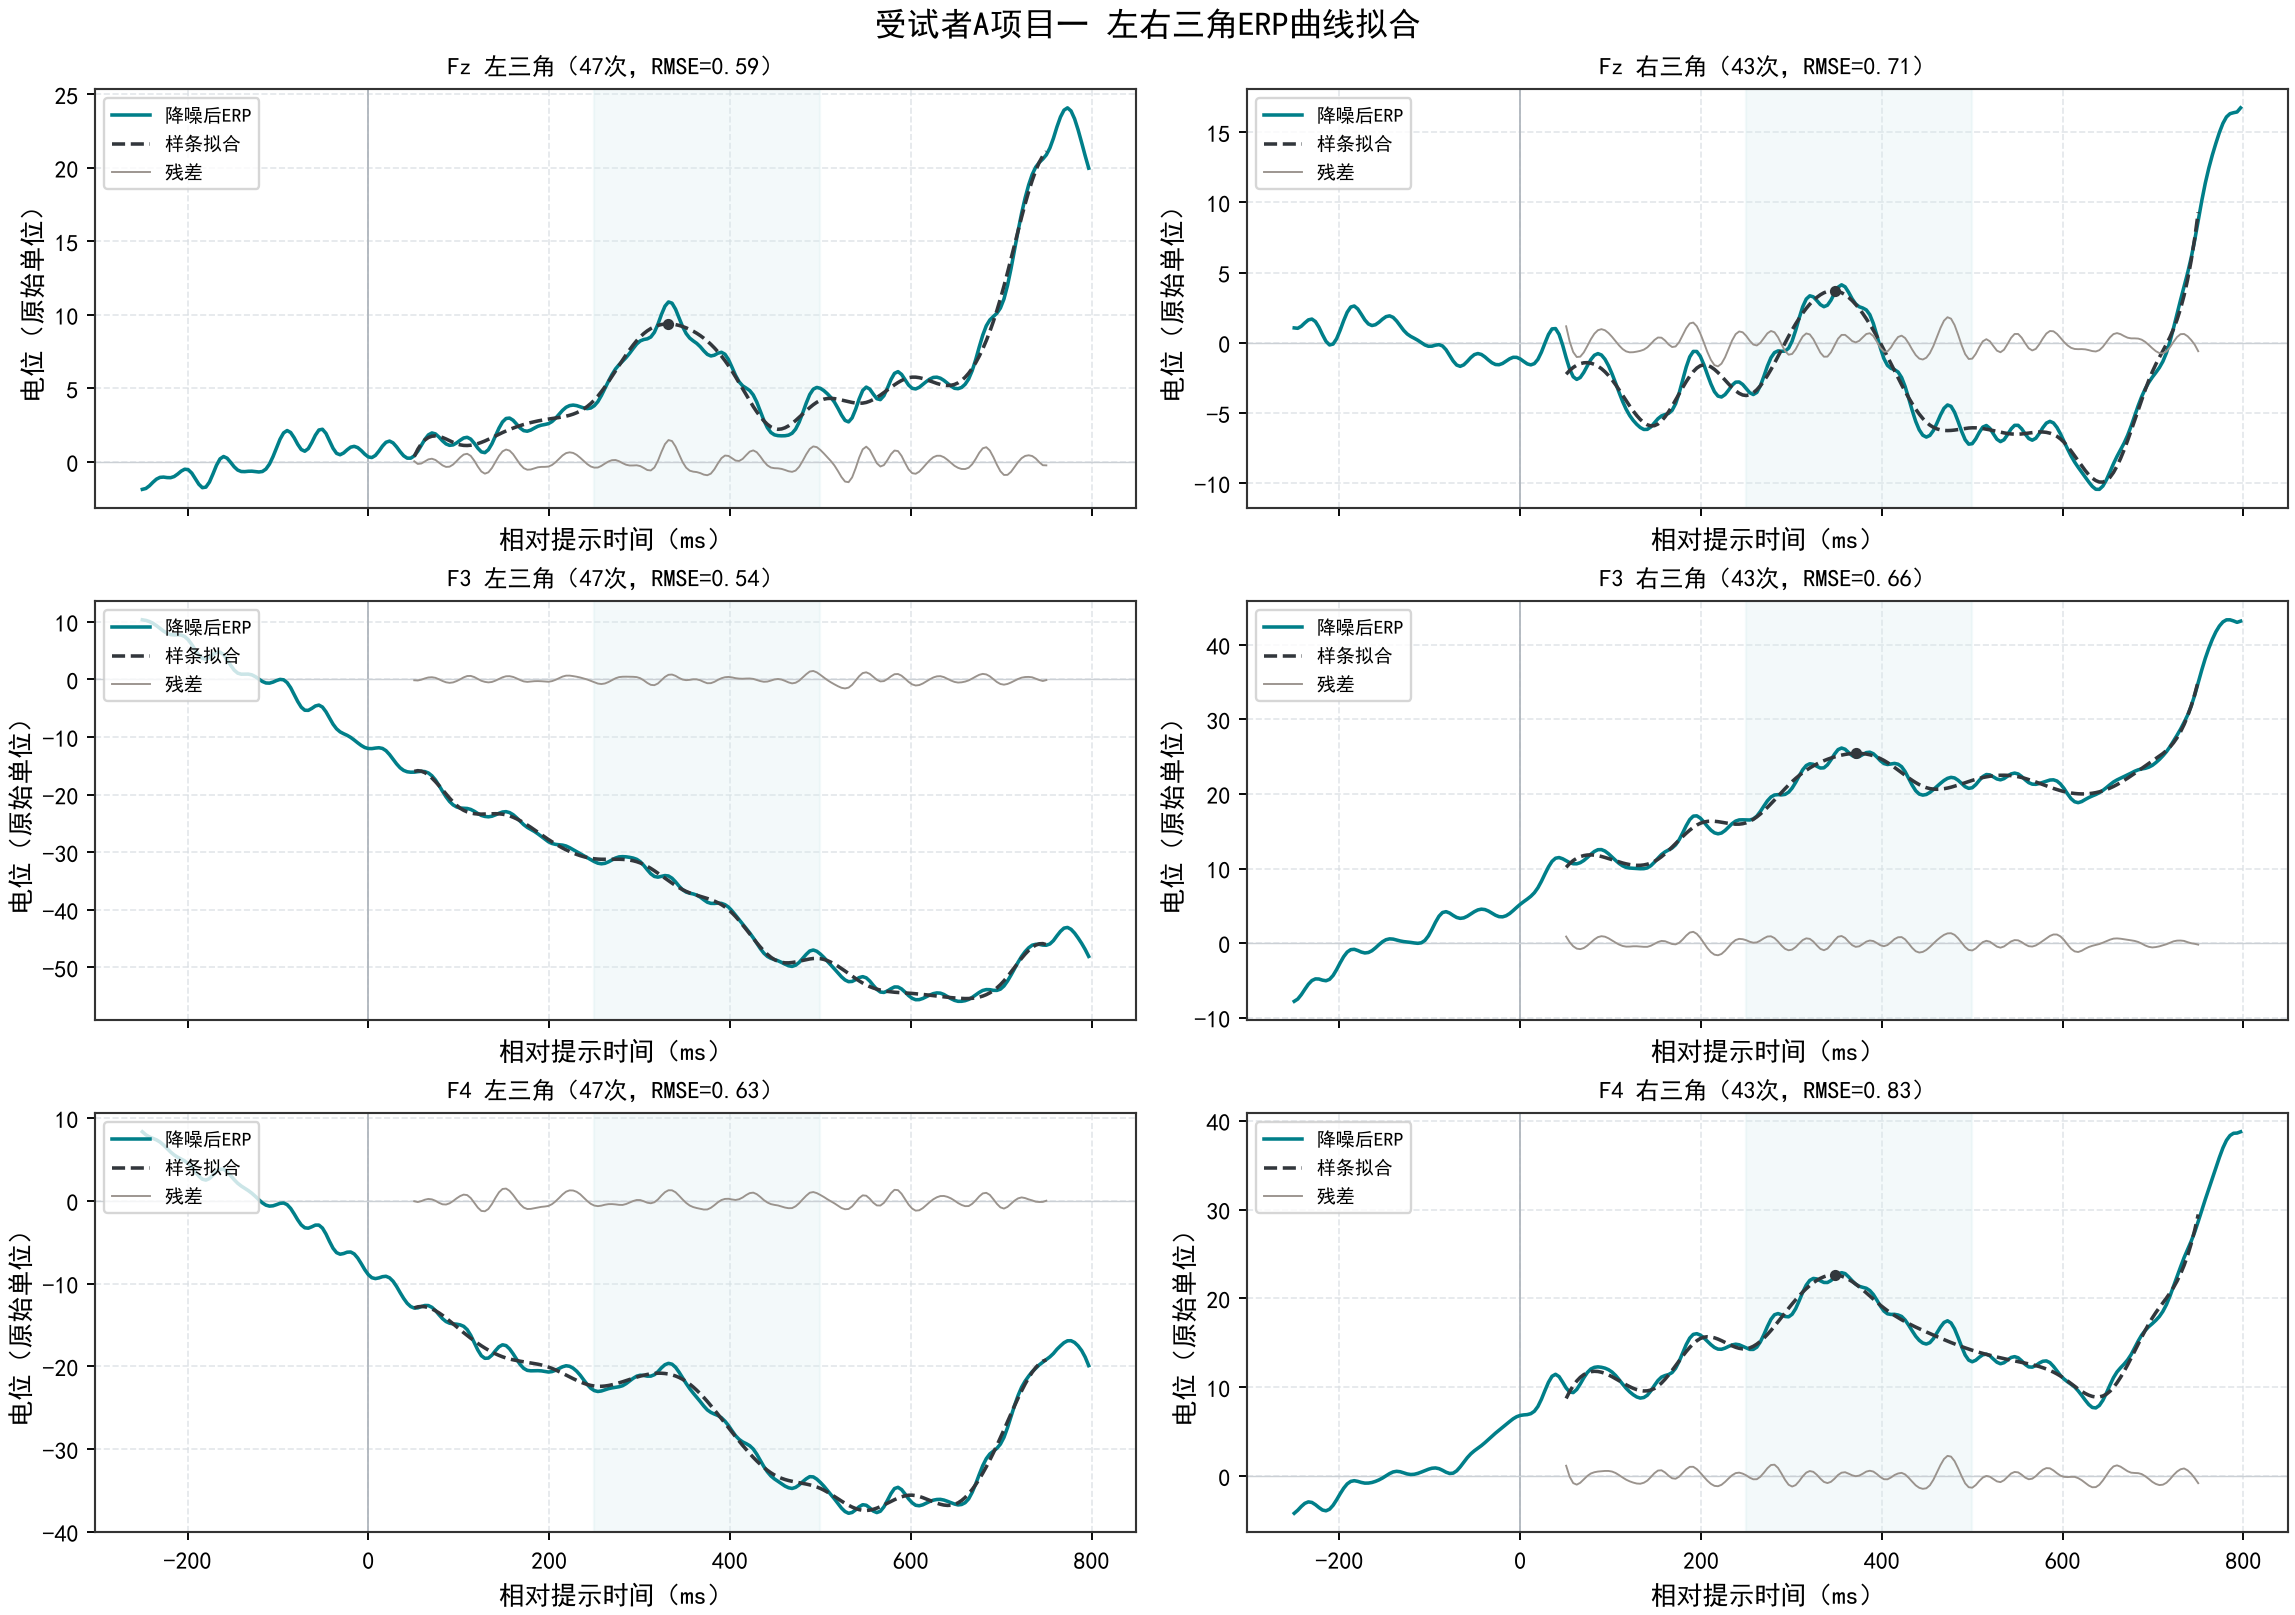
\includegraphics[width=0.95\textwidth]{q1_spline_a1.png}
    \caption{受试者 A 项目一左右条件 ERP 的三次 B 样条拟合与残差}
    \label{fig:q1_spline_example}
\end{figure}

\paragraph{（6）求解结果与稳健性检验}

四组数据的左右条件平均曲线如图~\ref{fig:q1_erp_all} 所示。实线与虚线分别表示校正后和预处理后 ERP，阴影区为 $250$--$500~\mathrm{ms}$ 分析窗。校正后曲线整体保留了处理前的主要低频形态，同时对部分试次间波动进行了收缩。四组数据的逐通道左右差分波形相关系数均值为 $0.992$--$0.998$，但将试次按时间顺序前后对半后，受试者 A 项目一和受试者 B 项目二的三通道差分相关分别为 $-0.322$ 和 $-0.400$，说明条件差异的跨时段稳定性尚未建立。

\begin{figure}[H]
    \centering
    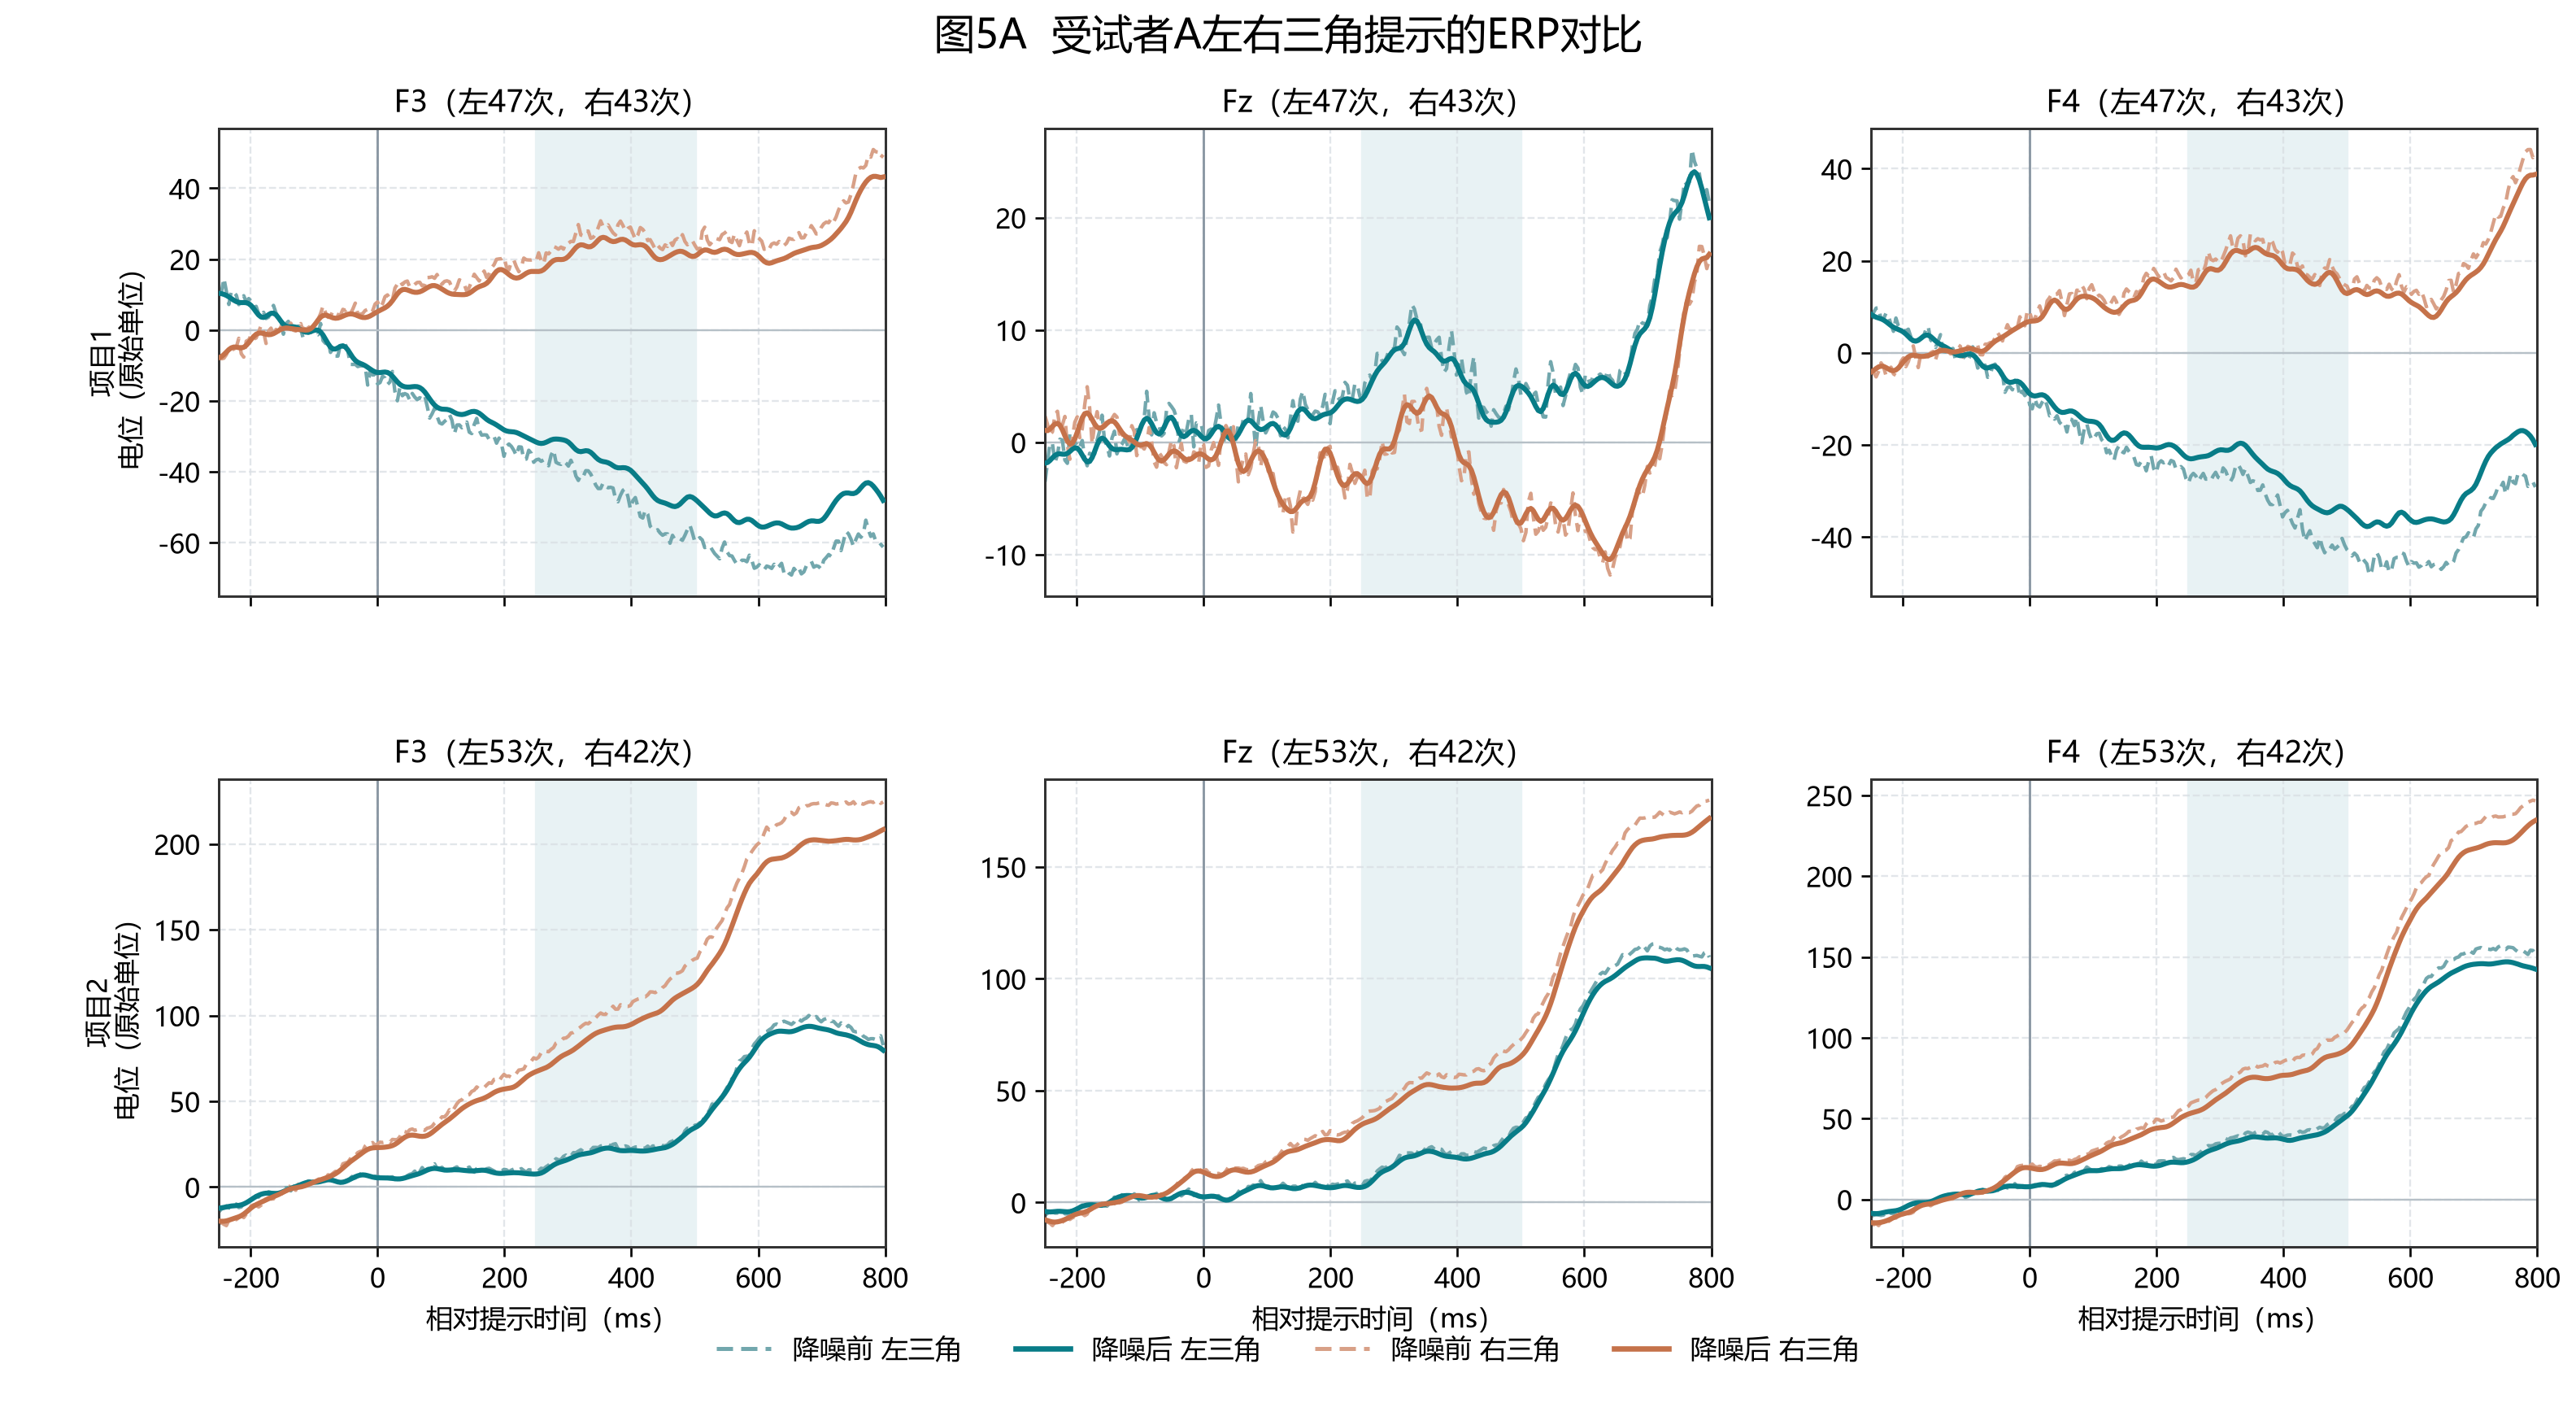
\includegraphics[width=0.94\textwidth]{q1_erp_a.png}\\[-0.3em]
    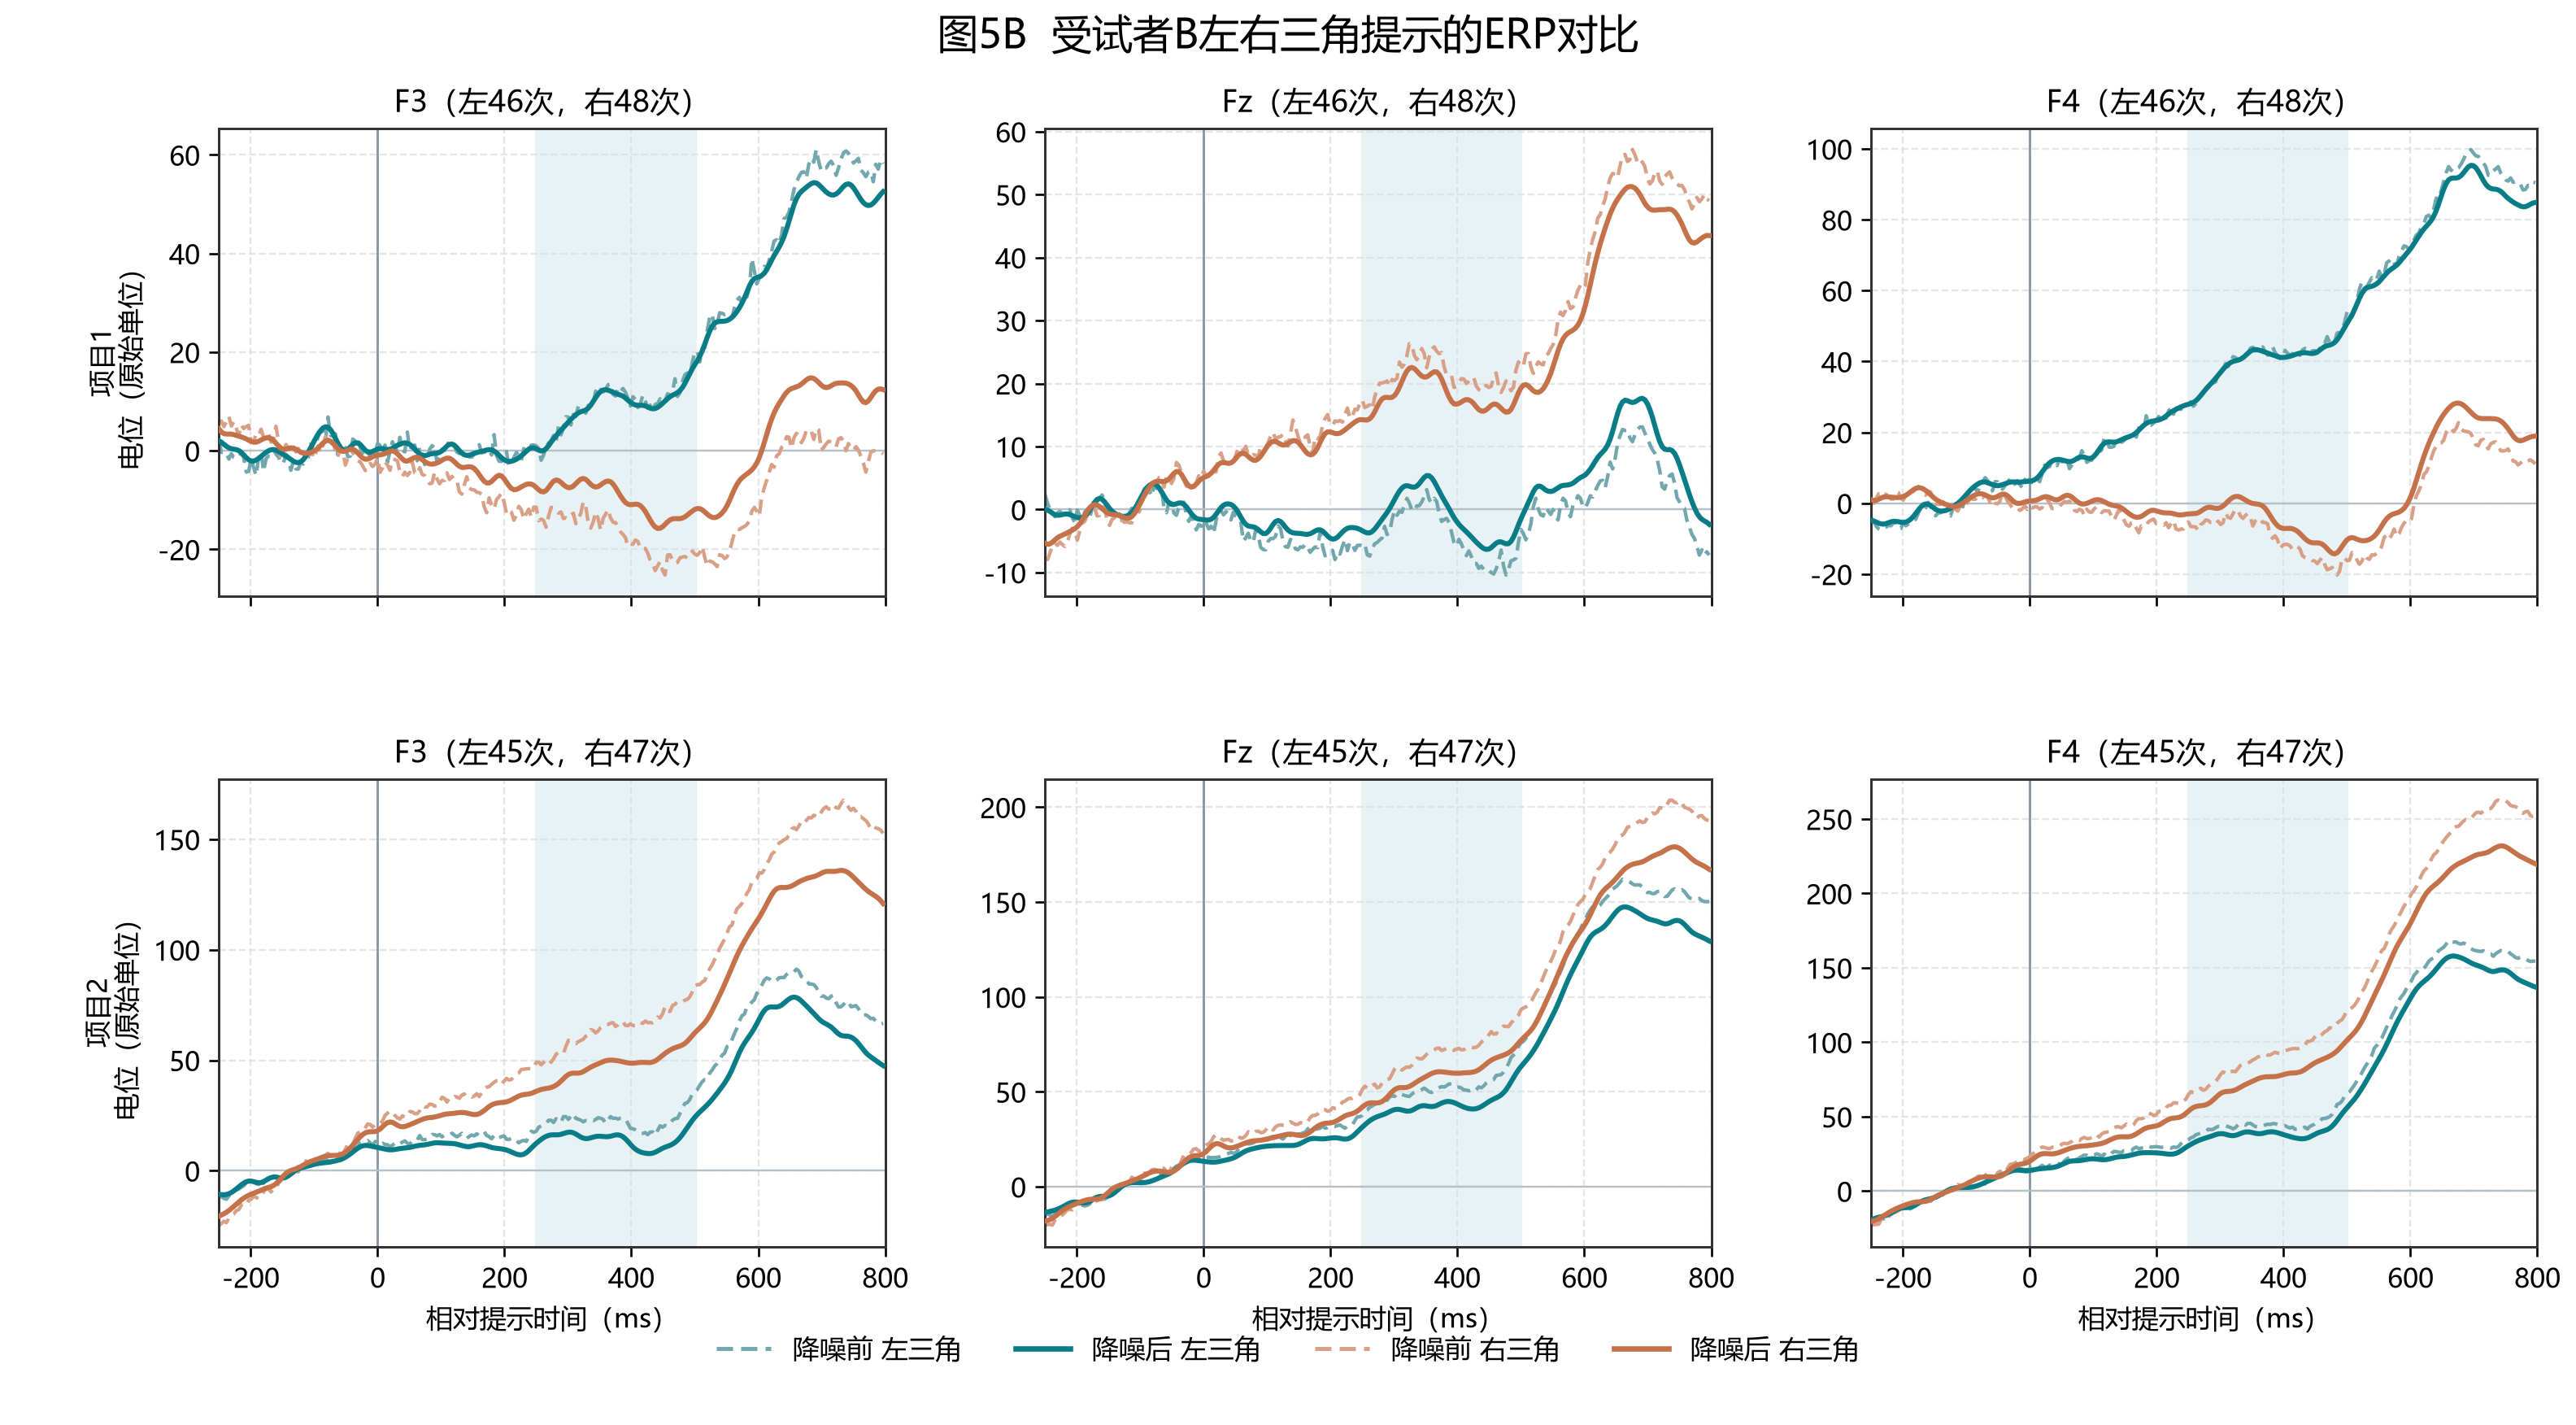
\includegraphics[width=0.94\textwidth]{q1_erp_b.png}
    \caption{受试者 A、B 在两个项目中的左右提示三通道 ERP 对比}
    \label{fig:q1_erp_all}
\end{figure}

进一步在真实测试背景上注入不同强度的瞬目样、扫视样和短暂运动样污染，结果如图~\ref{fig:q1_semisynthetic} 所示。强度为 $2$ 倍时，四组 V7 归一化 RMSE 相对未校正结果分别下降约 $9.9\%$、$11.6\%$、$10.8\%$ 和 $11.7\%$；但受试者 A 项目一在 $0.5$ 倍轻扰动下由 $0.174$ 上升至 $0.206$，且零注入时 V7 仍产生 $0.090$--$0.124$ 的背景改动。这表明模型更适合抑制较强的附加污染，不能保证每一种低强度场景均获得收益。

\begin{figure}[H]
    \centering
    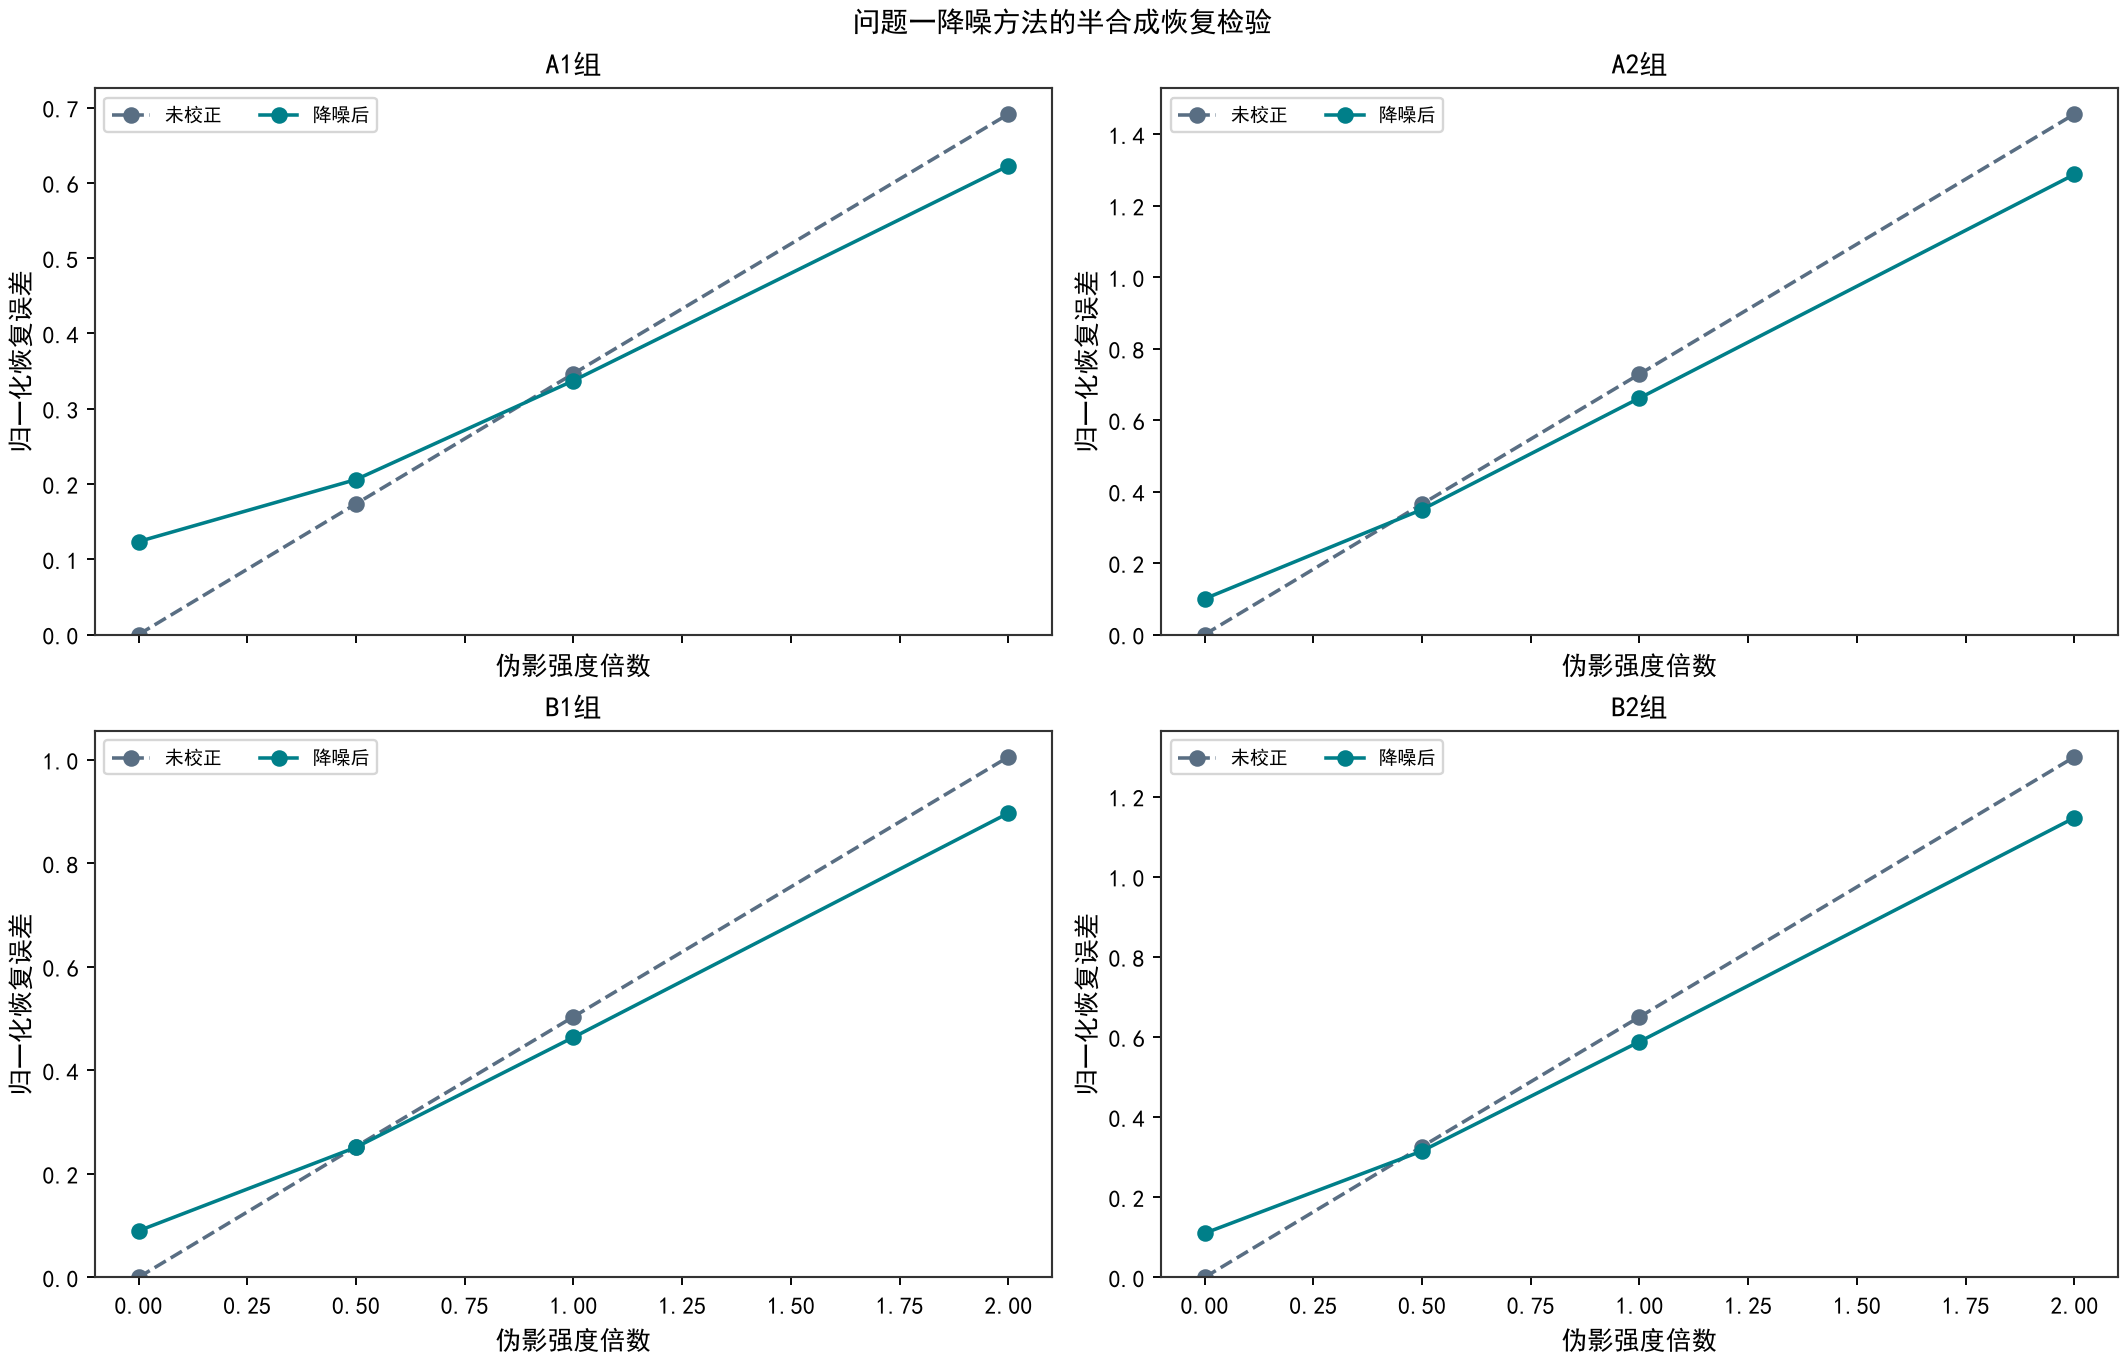
\includegraphics[width=0.92\textwidth]{q1_recovery.png}
    \caption{四组数据在不同伪影强度下的半合成恢复检验}
    \label{fig:q1_semisynthetic}
\end{figure}

综上，问题一得到了一套可复现的“原始通道预处理--折外自适应校正--条件 ERP 提取--样条拟合”求解方案。现有证据能够说明：在当前四组开发数据上，模型降低了相对训练代理模板的误差，并在较强人工污染下改善了恢复误差；现有证据不能单独证明：被保留的左右差异全部来自视觉神经活动、前额三通道已观测到典型中央--顶区 P300，或该方法能够直接完成未知方向识别。上述校正结果作为已知条件下的有效视觉响应，将为问题二的机理建模提供观测输入。

\renewcommand{\theequation}{2-\arabic{equation}}
\renewcommand{\theHequation}{q2.\arabic{equation}}
\setcounter{equation}{0}

\subsection{问题二模型的建立与求解}
\renewcommand{\theequation}{2-\arabic{equation}}
\renewcommand{\theHequation}{q2.\arabic{equation}}
\setcounter{equation}{0}

问题二要求由视觉刺激出发，建立贯通外侧膝状体核（LGN）、视皮层神经群与头皮脑电的正向计算模型，并据此解释左、右三角刺激所对应的脑电差异，进一步给出可供未知试次使用的特征表示。考虑到题给数据仅包含 Fz、F3、F4 三个前额通道，且未提供个体头模型、独立视觉源定位结果及同步眼动信息，本文不直接把头皮电位差异等同于某一脑区的唯一活动，而是构建“形状编码---群体动力学---突触等效源---条件共享观测”的可检验模型，将机制假设转化为可在独立时间块上验证的波形预测问题。

\subsubsection{建模思路}

\paragraph{（1）数据口径与预处理}

本问使用受试者 A、B 在项目一和项目二中的四组原始记录，分别记为 A1、A2、B1、B2。全部分析仅使用原始脑电通道 Fz、F3、F4，采样率为 $256~\mathrm{Hz}$；数据文件中的机器处理通道不作为“干净真值”，第 7 通道为心电通道，亦不将其误作眼电回归量。按照事件通道 VisCue 的符号，将 $-1$ 与 $+1$ 分别编码为左三角和右三角刺激。为兼顾刺激前基线和刺激后反应，截取每次提示前 $250~\mathrm{ms}$ 至提示后约 $800~\mathrm{ms}$ 的脑电片段。

连续记录先按时间顺序划分为 5 个互不重叠的时间块，再在每一块内独立完成 $0.1$--$30~\mathrm{Hz}$ 带通、$60~\mathrm{Hz}$ 陷波及提示前中位数基线校正。块边界两侧设置 $24~\mathrm{s}$ 保护区，防止双向滤波把测试块信息卷入训练块。经事件完整性、边界可用性和数值有效性检查后，四组记录分别保留 67、70、69、69 个试次，共 275 个试次，见表~\ref{tab:q2_trial_audit}。

\begin{table}[H]
\centering
\caption{问题二四组记录的数据审计与留出划分}
\label{tab:q2_trial_audit}
\begin{tabular}{ccccc}
\toprule
\textbf{记录} & \textbf{受试者} & \textbf{实验项目} & \textbf{有效试次数} & \textbf{连续时间块数} \\
\midrule
A1 & A & 项目一 & 67 & 5 \\
A2 & A & 项目二 & 70 & 5 \\
B1 & B & 项目一 & 69 & 5 \\
B2 & B & 项目二 & 69 & 5 \\
\midrule
\textbf{合计} & 2 人 & 2 个项目 & \textbf{275} & 20 \\
\bottomrule
\end{tabular}
\end{table}

在验证过程中，第 $k$ 个时间块只作为外层测试集，其余四块用于参数选择和观测矩阵估计。任何依赖类别均值、尺度分位数、缺失值填补或判别器参数的统计量，均只在训练块内计算后作用于测试块。由此，模型接受的是一个未知方向的原始试次，而非已经利用该试次标签构造的方向均值。

\paragraph{（2）总体技术路线}

本文采用“先建立可解释正向模型，再提炼可验证特征”的两阶段思路。第一阶段将左、右三角的镜像轮廓转化为三个形状偏好群的输入，经 LGN 中继和三级兴奋--抑制（E/I）神经群传播，得到九维突触等效源；随后用左右条件共享的观测矩阵映射到 Fz、F3、F4。第二阶段从单试次中提取时域幅值、峰值与潜伏期、空间侧化和机制模板投影等特征，并在连续时间块留出框架下检验其区分能力。

整体建模链路如图~\ref{fig:q2_model_pipeline} 所示。上排给出左右三角及两种反事实扰动，用于检查形状编码是否确由边缘组合驱动；下排展示从视觉边缘、LGN 中继、三级视觉皮层 E/I 神经群到突触源和头皮观测的计算路径。这里的三角图形依据题图示意进行标准化镜像构造，只承担模型输入编码作用，不将其解释为经过屏幕几何标定的真实刺激图像。

\begin{figure}[H]
\centering

\includegraphics[width=0.98\textwidth]{Q2_图1_机制与形状编码.pdf}
\caption{左右三角形状编码及脑电正向计算模型的总体路径}
\label{fig:q2_model_pipeline}
\end{figure}

\subsubsection{分层兴奋--抑制神经动力学模型的建立}

\paragraph{（1）视觉形状的空间边缘组合编码}

左、右三角具有镜像对称的轮廓结构。若只使用全图像素差，会使输入对位置和平移过于敏感，因此本文借鉴 COSFIRE 感受野的“定向边缘加空间组合”思想\cite{azzopardi2014ventral}。设标准化刺激图像为 $X_d(x,y)$，$d\in\{L,R\}$，$r_{\theta}(p;X_d)$ 表示在位置 $p$、方向 $\theta$ 上的边缘响应。对形状偏好群 $j\in\{L,R,0\}$，在 $K_j$ 个模板点上进行局部容差最大化，再以几何平均聚合：
\begin{equation}
f_j(X_d)=
\exp\!\left[
\frac{1}{K_j}\sum_{k=1}^{K_j}
\log\!\left(
\max_{\delta\in\mathcal N}
r_{\theta_{jk}}(p_{jk}+\delta;X_d)+\varepsilon
\right)\right],
\quad \varepsilon=10^{-6}.
\label{eq:q2_shape}
\end{equation}
其中，$L$、$R$ 分别表示左、右形状偏好群，$0$ 表示共同边缘群；$\mathcal N$ 为局部位移容差邻域。镜像刺激使得 $f_L(X_L)>f_R(X_L)$、$f_R(X_R)>f_L(X_R)$，但模型后续动力学参数在两种条件间完全共享，因而左右差异只能来自输入编码，而不能来自人为设置两套不同模型。

\paragraph{（2）LGN 中继与三级 E/I 神经群}

将形状编码向量记为 $\boldsymbol f(X_d)=[f_L,f_R,f_0]^{\mathsf T}$。LGN 中继状态 $\boldsymbol g(t)$ 接受有限持续时间的视觉驱动：
\begin{equation}
\tau_g\dot{\boldsymbol g}(t)
=-\boldsymbol g(t)+3\boldsymbol f(X_d)\,
\mathbb I_{[0,T_s)}(t),
\qquad T_s=\frac{52}{256}\ \mathrm{s}.
\label{eq:q2_lgn}
\end{equation}
为描述由早期视觉、中阶形状整合至额区响应的时序传递，构建三级 Wilson--Cowan 型神经群模型\cite{wilson1972excitatory,glomb2022computational}。令 $\boldsymbol E_s(t),\boldsymbol I_s(t)\in\mathbb R^3$ 分别为第 $s$ 级的兴奋性与抑制性群体状态，$s=1,2,3$，则
\begin{align}
\tau_{E,s}\dot{\boldsymbol E}_s
&=-\boldsymbol E_s+
\sigma\!\left(
\boldsymbol E_s-\boldsymbol I_s+
\rho\boldsymbol W\boldsymbol E_s+
\boldsymbol d_s-2\boldsymbol 1
\right), \label{eq:q2_e}\\
\tau_{I,s}\dot{\boldsymbol I}_s
&=-\boldsymbol I_s+
\sigma\!\left(
\boldsymbol E_s-\boldsymbol I_s-2\boldsymbol 1
\right), \label{eq:q2_i}\\
\boldsymbol d_1&=\boldsymbol g,\qquad
\boldsymbol d_s=3\!\left(
\boldsymbol E_{s-1}-\boldsymbol E_{s-1,0}
\right),\quad s=2,3. \label{eq:q2_feed}
\end{align}
式中，$\sigma(u)=1/(1+\mathrm e^{-u})$ 按元素作用，$\boldsymbol E_{s-1,0}$ 为静息状态；$\boldsymbol W$ 的主对角元为 0、非对角元为 $1/2$，用以表示同层不同形状偏好群之间的侧向复发耦合，$\rho$ 为复发强度。三级时间常数逐层增大，使模型可以表达早期快速感觉响应、中期形状整合及较慢额区响应，而不把三者压缩为一个无时延的线性映射。

图~\ref{fig:q2_cortex_response} 以 A1 为例展示完整模型内部状态。灰色区为视觉驱动时段；从早期视觉层到形状整合层、再到额区响应层，兴奋性状态和突触等效源的峰值逐级后移。蓝、红两线的分离首先出现在与输入方向一致的形状偏好群，并随级联传播至后续层级。这一结果说明模型内部确能把镜像轮廓差异转化为具有时延的动态差异，但它本身仍属于模型结构结果，不能单独证明相应神经群已被实际观测。

\begin{figure}[H]
\centering

\includegraphics[width=0.98\textwidth]{Q2_图2_皮层内部响应.pdf}
\caption{A1 记录对应的三级 E/I 神经群及突触等效源响应}
\label{fig:q2_cortex_response}
\end{figure}

\paragraph{（3）突触等效源与头皮观测}

头皮脑电主要反映大规模同步突触后电流，而非单个神经元动作电位\cite{steeghs2025slow}。因此，对每一级兴奋、抑制状态分别施加二阶低通突触核：
\begin{align}
\tau_{e,s}\dot{\boldsymbol u}_{e,s}
&=\boldsymbol E_s-\boldsymbol E_{s,0}-\boldsymbol u_{e,s},
&
\tau_{e,s}\dot{\boldsymbol v}_{e,s}
&=\boldsymbol u_{e,s}-\boldsymbol v_{e,s}, \label{eq:q2_syn_e}\\
\tau_{i,s}\dot{\boldsymbol u}_{i,s}
&=\boldsymbol I_s-\boldsymbol I_{s,0}-\boldsymbol u_{i,s},
&
\tau_{i,s}\dot{\boldsymbol v}_{i,s}
&=\boldsymbol u_{i,s}-\boldsymbol v_{i,s}. \label{eq:q2_syn_i}
\end{align}
第 $s$ 级的突触等效源定义为
\begin{equation}
\boldsymbol q_s(t)=
\boldsymbol v_{e,s}(t)-0.7\boldsymbol v_{i,s}(t).
\label{eq:q2_source}
\end{equation}
将三级、三群的源活动拼接为九维向量 $\boldsymbol q(t)\in\mathbb R^9$，并施加与实测脑电相同的滤波和基线处理，得到 $\widetilde{\boldsymbol q}(t)$。Fz、F3、F4 的预测向量为
\begin{equation}
\widehat{\boldsymbol y}_d(t)
=\boldsymbol L\,\widetilde{\boldsymbol q}_d(t),
\qquad
\widehat{\boldsymbol y}_d(t)\in\mathbb R^3,\quad
\boldsymbol L\in\mathbb R^{3\times 9}.
\label{eq:q2_observation}
\end{equation}
由于缺少个体 MRI 和电导率头模型，$\boldsymbol L$ 被定义为训练块内估计的“有效观测矩阵”，而非可直接对应解剖位置的物理导联场。为了同时拟合两种条件共有的 ERP 背景与较弱的方向差异，定义
\[
\boldsymbol C_y=\frac{\boldsymbol y_R+\boldsymbol y_L}{2},
\qquad
\boldsymbol D_y=\boldsymbol y_R-\boldsymbol y_L,
\]
并对源信号构造相应的 $\boldsymbol C_q,\boldsymbol D_q$。条件共享观测矩阵通过下式求解：
\begin{equation}
\widehat{\boldsymbol L}
=\arg\min_{\boldsymbol L}
\left\{
\frac12\|\boldsymbol C_y-\boldsymbol L\boldsymbol C_q\|_{\boldsymbol W_t}^{2}
+\frac12\|\boldsymbol D_y-\boldsymbol L\boldsymbol D_q\|_{\boldsymbol W_t}^{2}
+\lambda\|\boldsymbol L\|_F^2
\right\}.
\label{eq:q2_readout}
\end{equation}
时间权重 $\boldsymbol W_t$ 对 $50$--$250~\mathrm{ms}$、$250$--$500~\mathrm{ms}$ 和 $500$--$750~\mathrm{ms}$ 三个分析窗等权赋值，避免样本点数不同使某一时间窗主导目标函数。

\paragraph{（4）参数选择与数值求解}

模型微分方程按 $256~\mathrm{Hz}$ 的时间网格数值积分。固定参数用于描述逐层变慢的群体与突触过程；全局时间尺度、复发强度和岭参数则仅在外层训练块中选择，具体见表~\ref{tab:q2_params}。

\begin{table}[H]
\centering
\caption{问题二神经动力学模型的主要参数}
\label{tab:q2_params}
\resizebox{\textwidth}{!}{%
\begin{tabular}{llll}
\toprule
\textbf{参数} & \textbf{含义} & \textbf{候选值或设定} & \textbf{确定方式} \\
\midrule
$\tau_g$ & LGN 中继时间常数 & $20\times\mathrm{scale}~\mathrm{ms}$ & 层级时间先验 \\
$\tau_{E,1:3}$ & 三级兴奋群时间常数 & $[20,40,80]\times\mathrm{scale}~\mathrm{ms}$ & 层级时间先验 \\
$\tau_{I,1:3}$ & 三级抑制群时间常数 & $[40,80,160]\times\mathrm{scale}~\mathrm{ms}$ & 层级时间先验 \\
$\tau_{e,1:3}$ & 兴奋性突触时间常数 & $[25,50,100]\times\mathrm{scale}~\mathrm{ms}$ & 突触核设定 \\
$\tau_{i,1:3}$ & 抑制性突触时间常数 & $[75,150,300]\times\mathrm{scale}~\mathrm{ms}$ & 慢抑制设定 \\
$\mathrm{scale}$ & 全局时间尺度 & $\{0.75,1.00,1.25\}$ & 训练块内选择 \\
$\rho$ & 同层复发强度 & $\{0,0.1,0.2\}$ & 训练块内选择 \\
$\lambda$ & 观测矩阵岭参数 & $\{0.1,0.3,1,3,10,30,100\}$ & 训练块内选择 \\
\bottomrule
\end{tabular}}
\end{table}

图~\ref{fig:q2_erp_fitting} 给出 A1 的同样本描述拟合和五个外层留出块的等权汇总。实线为观测 ERP，虚线为模型预测。上排用于观察模型在训练信息充分时可表示的波形形态，下排用于评价模型的外推能力。结果显示，模型能够生成与视觉提示同步、并在三通道呈现不同符号和尺度的预测；对于 F3、F4 中幅值较大的慢变成分，模型仍有进一步细化空间，因此后续重点结合留出结果评价其解释能力。

\begin{figure}[H]
\centering

\includegraphics[width=0.98\textwidth]{Q2_图3_ERP拟合与留出.pdf}
\caption{A1 左右条件 ERP 的同样本描述拟合与连续时间块留出预测}
\label{fig:q2_erp_fitting}
\end{figure}

\subsubsection{脑电信号差异的模型解释}

\paragraph{（1）左右差异的形成路径}

在模型中，左右刺激之间的差异沿如下路径形成：镜像轮廓首先改变式~\eqref{eq:q2_shape} 中的形状偏好输入；该差异经式~\eqref{eq:q2_lgn} 的 LGN 中继进入三级 E/I 网络，在不同时间常数作用下形成逐层延迟的源活动；最后由同一个 $\widehat{\boldsymbol L}$ 投影为三通道电位。由于动力学参数和观测矩阵对左右条件共享，模型不允许通过“给左、右条件分别拟合一套参数”来制造差异。

为检验预测差异是否优于“左右完全相同”的平凡模型，定义右减左差异波
\[
\boldsymbol D^{\mathrm{obs}}(t)
=\boldsymbol y_R(t)-\boldsymbol y_L(t),\qquad
\boldsymbol D^{\mathrm{pred}}(t)
=\widehat{\boldsymbol y}_R(t)-\widehat{\boldsymbol y}_L(t),
\]
并构造差分预测增益
\begin{equation}
S_\Delta
=1-
\frac{\operatorname{MSE}
\!\left(\boldsymbol D^{\mathrm{obs}},\boldsymbol D^{\mathrm{pred}}\right)}
{\operatorname{MSE}
\!\left(\boldsymbol D^{\mathrm{obs}},\boldsymbol 0\right)}.
\label{eq:q2_sdelta}
\end{equation}
当 $S_\Delta>0$ 时，模型在该记录上的差异预测优于零差异基准；$S_\Delta<0$ 表明当前参数配置相对零差异基准的增益较为有限。该指标是相对于零差异基准的预测增益，不等同于常规定义的决定系数 $R^2$。

\paragraph{（2）独立留出差异波结果}

四组记录的留出差异波如图~\ref{fig:q2_diff_waves} 所示。蓝色实线为实测右减左差异，红色虚线为模型预测，浅蓝阴影为块重采样得到的点态区间。A2、B2 在部分分析窗内能够跟踪差异波的方向和缓慢变化；A1、B1 的预测在部分时段与观测幅值存在偏差。随时间增大的区间宽度进一步反映了慢漂移和试次间波动对差异波估计的影响。

\begin{figure}[H]
\centering

\includegraphics[width=0.78\textwidth]{Q2_图4_左右差异波.pdf}
\caption{四组记录右减左 ERP 差异波的连续时间块留出预测}
\label{fig:q2_diff_waves}
\end{figure}

表~\ref{tab:q2_mechanism_results} 给出各记录的定量结果。A1、B2 的 $S_\Delta$ 点估计为正，表明模型在这两组记录上捕捉到了优于零差异基准的方向变化；A2、B1 的点估计相对接近基准，且块重采样区间整体较宽。综合来看，该模型已呈现一定的差异波外推能力，其跨记录稳定性仍有进一步提升空间。

\begin{table}[H]
\centering
\caption{完整模型在四组记录上的留出预测结果}
\label{tab:q2_mechanism_results}
\resizebox{\textwidth}{!}{%
\begin{tabular}{lccccc}
\toprule
\textbf{记录} & \textbf{$S_\Delta$} & \textbf{$S_\Delta$ 块重采样区间} &
\textbf{差异 RMSE} & \textbf{总 ERP $R^2$} & \textbf{波形相关系数} \\
\midrule
A1 & 0.0581 & $[-0.4743,\ 0.1474]$ & 91.1154 & $-0.1825$ & $-0.5342$ \\
A2 & $-0.0842$ & $[-1.0452,\ 0.4769]$ & 87.6182 & 0.1283 & 0.4166 \\
B1 & $-0.0176$ & $[-0.0699,\ -0.0004]$ & 98.3928 & $-0.1027$ & $-0.1545$ \\
B2 & 0.2562 & $[-1.1102,\ 0.5607]$ & 90.6075 & $-0.1176$ & 0.1193 \\
\bottomrule
\end{tabular}}
\end{table}

\paragraph{（3）额区空间侧化的解释}

为描述双侧额区相对变化，在 $250$--$500~\mathrm{ms}$ 时窗内记三通道平均幅值为 $A_{\mathrm{Fz}},A_{\mathrm{F3}},A_{\mathrm{F4}}$，定义稳定化侧化指数
\begin{equation}
\mathrm{LI}
=\frac{A_{\mathrm{F4}}-A_{\mathrm{F3}}}
{\max\!\left(
|A_{\mathrm{F4}}|+|A_{\mathrm{F3}}|,
\epsilon_{\mathrm{train}}
\right)}.
\label{eq:q2_li}
\end{equation}
其中，$\epsilon_{\mathrm{train}}$ 由训练块幅值尺度的低分位数确定，用于防止分母接近零。图~\ref{fig:q2_lateralization} 的左、中列分别给出 F4--F3 电位差和 LI 的实测/预测曲线，右列给出分析窗内单试次 LI 分布。不同记录中的极性与幅值呈现一定个体差异，因此额区侧化更适合作为候选空间特征；其生理含义还需结合眼动、任务准备、参考电极及个体体传导差异进行综合分析。

\begin{figure}[H]
\centering

\includegraphics[width=0.98\textwidth]{Q2_图5_空间侧化.pdf}
\caption{四组记录的 F4--F3 电位差与稳定化侧化指数}
\label{fig:q2_lateralization}
\end{figure}

\paragraph{（4）消融与敏感性分析}

为判定预测结果依赖模型中的哪些结构，分别进行三类反事实消融：令 $f_L=f_R$ 以取消形状选择性；令 $\rho=0$ 以取消同层跨群复发；约束 F3、F4 观测行对称以取消观测侧化。同时，将时间尺度、复发强度及 F4 读出权重在固定范围内扰动，考察 $S_\Delta$ 的变化。

图~\ref{fig:q2_ablation} 左上给出完整模型和多种替代模型的留出增益，右上为三项消融后的误差变化，左下为参数敏感性，右下为完整模型的块重采样区间。取消形状后模型的方向输出按结构归零，表明“形状选择性输入”是模型内部产生左右差异的必要条件；复发和对称观测消融在不同记录上呈现不同影响，反映了各结构对个体记录的贡献存在差异。A2、B2 的区间相对较宽，后续可通过增加重复记录进一步提高消融效应估计的精度。

\begin{figure}[H]
\centering

\includegraphics[width=0.98\textwidth]{Q2_图6_消融与敏感性.pdf}
\caption{模型消融、固定参数干预及差异预测增益的敏感性分析}
\label{fig:q2_ablation}
\end{figure}

\paragraph{（5）模型解释的证据边界}

综上，本模型形成了三层递进结果。第一，形状编码和级联动力学在数学上给出一条可计算的差异形成路径；第二，A1、B2 的正 $S_\Delta$ 表明该路径在部分记录上具有超越零差异基准的留出预测价值；第三，A2、B1 的点估计及较宽区间提示模型在跨记录适配方面仍有优化空间。考虑到现有观测通道数量和辅助信息条件，本文将 LGN、视觉层和额区层作为功能性计算模块，用于提供可解释的正向建模框架；更精细的解剖定位可在后续结合个体头模型、眼动与多通道数据进一步验证。

\subsubsection{视觉刺激响应的特征表示}

\paragraph{（1）二十三维机制增强特征}

为将正向模型转化为可供未知试次使用的表示，在每个试次上构造
\begin{equation}
\boldsymbol\phi
=
\left[
\boldsymbol A_{1:3},
\boldsymbol P_{1:3},
\boldsymbol T_{1:3},
\boldsymbol M_{1:3},
\mathrm{LI},
A_{\mathrm{F4}}-A_{\mathrm{F3}},
\boldsymbol b_{1:6},
\boldsymbol e_{1:3}
\right]^{\mathsf T}
\in\mathbb R^{23}.
\label{eq:q2_feature}
\end{equation}
各分量的定义见表~\ref{tab:q2_feature_def}。其中，$\boldsymbol b$ 为单试次在训练块共同模板和差异模板上的最小二乘投影系数，$\boldsymbol e$ 为相应的通道重构残差。构造测试试次特征时只使用训练块模板，不读取该试次的真实方向，因此该表示可用于严格的未知方向预测。

\begin{table}[H]
\centering
\caption{二十三维视觉刺激响应特征的组成}
\label{tab:q2_feature_def}
\resizebox{\textwidth}{!}{%
\begin{tabular}{lccl}
\toprule
\textbf{特征组} & \textbf{维数} & \textbf{计算区间或定义} & \textbf{表征含义} \\
\midrule
$\boldsymbol A_{1:3}$ & 3 & $250$--$500~\mathrm{ms}$ 三通道有符号均值 & 中期响应幅值 \\
$\boldsymbol P_{1:3}$ & 3 & 窗内满足阈值的局部正峰 & 峰值强度 \\
$\boldsymbol T_{1:3}$ & 3 & 有效正峰的潜伏期 & 反应时序 \\
$\boldsymbol M_{1:3}$ & 3 & 无合格峰时取 1 & 峰缺失状态 \\
$\mathrm{LI}$ & 1 & 式~\eqref{eq:q2_li} & 稳定化额区侧化 \\
$A_{\mathrm{F4}}-A_{\mathrm{F3}}$ & 1 & 分析窗内 F4 与 F3 幅值差 & 双侧额区梯度 \\
$\boldsymbol b_{1:6}$ & 6 & 训练块共同/差异模板投影 & 机制模板坐标 \\
$\boldsymbol e_{1:3}$ & 3 & $50$--$750~\mathrm{ms}$ 通道重构 RMS & 模型未解释成分 \\
\midrule
\textbf{合计} & \textbf{23} & --- & 时域、空间与机制信息联合表示 \\
\bottomrule
\end{tabular}}
\end{table}

\paragraph{（2）判别器与评价指标}

对每个特征组使用收缩协方差线性判别分析。训练块内估计类别均值 $\boldsymbol\mu_L,\boldsymbol\mu_R$ 和收缩协方差 $\widehat{\boldsymbol\Sigma}_\gamma$，对未知试次 $\boldsymbol\phi$ 的判别函数写为
\begin{equation}
h(\boldsymbol\phi)
=
\left(\boldsymbol\mu_R-\boldsymbol\mu_L\right)^{\mathsf T}
\widehat{\boldsymbol\Sigma}_{\gamma}^{-1}\boldsymbol\phi
-\frac12
\left(
\boldsymbol\mu_R^{\mathsf T}
\widehat{\boldsymbol\Sigma}_{\gamma}^{-1}\boldsymbol\mu_R
-
\boldsymbol\mu_L^{\mathsf T}
\widehat{\boldsymbol\Sigma}_{\gamma}^{-1}\boldsymbol\mu_L
\right).
\label{eq:q2_lda}
\end{equation}
以平衡准确率
\begin{equation}
\mathrm{BA}
=\frac12
\left(
\frac{\mathrm{TP}}{\mathrm{TP}+\mathrm{FN}}
+
\frac{\mathrm{TN}}{\mathrm{TN}+\mathrm{FP}}
\right)
\label{eq:q2_ba}
\end{equation}
作为主指标，并同时报告 AUC 与 F1。置信区间采用 1000 次连续块重采样；原假设检验在每个时间块内部置换标签 1999 次，以保留块内类别数和时间结构；七组特征之间再使用 maxT 对多重比较进行校正。另以 199 次块内循环移位作为时间依赖稳健性检查。

\paragraph{（3）留出判别结果}

表~\ref{tab:q2_feature_performance} 汇总全部 275 个试次的外层留出结果。幅值特征取得最高的观测 BA 0.5161，其 95\% 块重采样区间覆盖 0.5，maxT 校正后 $p=0.7855$；23 维机制增强特征的 BA 为 0.4471、AUC 为 0.4679，校正后 $p=0.9995$。峰潜伏期、空间侧化和协方差投影等特征的结果主要分布在机会水平附近，表明在当前样本规模下，单试次方向信息的可分程度相对有限。

\begin{table}[H]
\centering
\caption{不同视觉刺激响应特征的连续时间块留出判别性能}
\label{tab:q2_feature_performance}
\resizebox{\textwidth}{!}{%
\begin{tabular}{lccccc}
\toprule
\textbf{特征组} & \textbf{BA} & \textbf{BA 块重采样区间} &
\textbf{AUC} & \textbf{F1} & \textbf{maxT 校正 $p$ 值} \\
\midrule
时域幅值（amplitude） & 0.5161 & $[0.4846,\ 0.5481]$ & 0.5337 & 0.5056 & 0.7855 \\
峰潜伏期（peak\_latency） & 0.4690 & $[0.4200,\ 0.5159]$ & 0.4663 & 0.4632 & 0.9960 \\
空间侧化（spatial） & 0.4693 & $[0.4332,\ 0.5004]$ & 0.4721 & 0.4710 & 0.9960 \\
23 维机制特征（mechanism） & 0.4471 & $[0.4016,\ 0.4837]$ & 0.4679 & 0.4370 & 0.9995 \\
协方差特征（covariance） & 0.4692 & $[0.4221,\ 0.5208]$ & 0.4770 & 0.4672 & 0.9960 \\
六维投影（projection6） & 0.4840 & $[0.4521,\ 0.5205]$ & 0.4896 & --- & 0.9795 \\
三维方向投影（direction3） & 0.4919 & $[0.4451,\ 0.5378]$ & 0.4632 & --- & 0.9535 \\
\bottomrule
\end{tabular}}
\end{table}

图~\ref{fig:q2_classification} 以 A1 为例给出 PCA 投影、各特征组留出 BA、机制特征混淆矩阵以及置换零分布。PCA 图中的训练点存在局部聚集，测试点则保留一定重叠；观测 BA 的红线落在置换分布主体内，与校正 $p$ 值一致。机制特征相对空间特征的 BA 差值为 $-2.2$ 个百分点，块重采样区间为 $[-4.9,\ 0.3]$ 个百分点，说明其当前增量收益较为有限，后续可通过丰富观测通道和扩大训练样本进一步提升。

\begin{figure}[H]
\centering

\includegraphics[width=0.98\textwidth]{Q2_图7_特征与判别.pdf}
\caption{A1 视觉刺激特征投影、留出判别与块内置换检验}
\label{fig:q2_classification}
\end{figure}

\paragraph{（4）特征表示的使用结论}

由上述结果可知，式~\eqref{eq:q2_feature} 给出了一个计算闭合、对未知试次无标签泄漏的视觉刺激响应表示，可作为后续脑机接口模型的候选输入。现有两名受试者、四组记录和三个额区通道已呈现幅值、侧化与机制投影等多类候选差异，但单试次层面的区分度仍有提升空间。后续可通过增加受试者与重复记录，引入枕区/顶区电极和同步眼动通道，并在独立采集批次上固定时间窗、参数网格和最终判别器，以进一步提高特征表示的稳定性和迁移能力。
\subsection{问题三模型的建立与求解}

问题三要求在视觉提示、候选目标与应答行为之间建立连续的认知过程模型。为避免把应答后的动作电位混入认知状态，本文首先审计四组记录的事件语义，并按“应答前约 $100~\mathrm{ms}$”原则构造变长脑电窗口；随后继承问题二的形状编码与视觉群体动力学，将提示保持、目标触发提取和认知整合表示为低维功能状态，再通过训练块内估计的有效观测矩阵映射至 $F_z$、$F_3$、$F_4$；最后以认知差分状态驱动随机证据累积过程，统一表示正确、错误和有限观察期内未决三类结局。真实 EEG 用于检验波形预测，仿真轨迹用于检验模型能否产生题目所述的异常应答情形，二者在解释上严格区分。

\subsubsection{建模思路}

\paragraph{（1）从事件证据到认知状态的分层建模}

本问采用“事件层---认知层---观测层---决策层”的递进结构。事件层确定提示、目标和应答的时间边界；认知层描述视觉输入在短时保持与目标触发下的状态演化；观测层把模型状态投影为头皮电位；决策层仅在仿真任务布局中把方向证据转换为行为结局。各层的输入、状态与输出如表~\ref{tab:q3_route} 所示。该结构一方面复用问题二已建立的视觉通路，另一方面将无法由三导联 EEG 直接确认的深部来源保留为功能性状态，而不将其解释为海马体的直接源定位结果\cite{glomb2022computational,daume2024control}。

\begin{table}[H]
\centering
\caption{问题三认知模型的分层结构}
\label{tab:q3_route}
\resizebox{\textwidth}{!}{%
\begin{tabular}{llll}
\toprule
\textbf{模型层次} & \textbf{主要输入} & \textbf{核心状态或运算} & \textbf{输出及作用} \\
\midrule
事件层 & VisCue、TgtAct、记录边界 & 事件审计与应答前截窗 & 合格的变长认知脑电片段 \\
视觉--认知层 & 提示形状、目标出现时刻 & 视觉输入 $\boldsymbol v$、记忆状态 $\boldsymbol m$、认知状态 $\boldsymbol p$ & 连续认知源时间序列 \\
头皮观测层 & 认知源与提示前背景 & 条件共享有效观测矩阵 & 三通道预测脑电 $\widehat{\boldsymbol x}$ \\
行为决策层 & 方向对齐认知证据 & 有界随机证据累积 & 正确、错误与未决三类仿真结局 \\
验证层 & 留出时间块与保存结果 & 误差比较、消融及敏感性分析 & 模型适用范围与证据边界 \\
\bottomrule
\end{tabular}}
\end{table}

\paragraph{（2）数据隔离与模型求解原则}

每组 100 个提示事件按原始时间顺序划分为 5 个连续时间块。第 $k$ 个时间块仅作为外层测试集，其余 4 个时间块用于选择时间常数、目标输入持续时间和岭惩罚强度，并估计头皮观测系数。任何由均值、尺度、背景斜率或候选参数产生的统计量均在训练块内部计算后作用于测试块。由此，模型接受的是一条未见过的原始认知试次，而不是已经利用该试次应答信息构造的条件平均波形。

模型求解依次完成四个步骤：首先确定每次试验可用的认知窗口；其次由问题二模型生成提示与目标的视觉驱动；再次联合求解低维认知状态和三通道观测映射；最后在固定认知状态上进行决策仿真、消融检验和观察窗敏感性分析。该路线对应“信号截取---状态建模---参数估计---外层验证”的闭环，能够分别回答认知信号如何截取、模型状态如何形成、头皮脑电如何观测以及异常应答如何处理。

\paragraph{（3）候选模型与对照体系}

为判断模型性能来自视觉瞬态、缓慢背景还是提示保持结构，本文不只拟合单一模型，而是建立由简到繁的候选族。各候选共享同一事件窗口、因果滤波、外层划分和评价指标，仅改变进入设计矩阵的状态列，因此模型间误差可以在相同测试试次上逐项比较。主模型记为 N2，其余候选分别承担零输入基准、视觉瞬态基准、单级认知基准和慢趋势对照等作用；同时通过删除记忆投影或关闭提取门，检验 N2 中各环节是否确有贡献。具体关系见表~\ref{tab:q3_candidates}。

\begin{table}[H]
\centering
\caption{问题三候选模型与对照关系}
\label{tab:q3_candidates}
\resizebox{\textwidth}{!}{%
\begin{tabular}{clll}
\toprule
\textbf{模型} & \textbf{保留的状态} & \textbf{主要用途} & \textbf{解释边界} \\
\midrule
B0 & 不含刺激状态，仅保留提示前背景外推 & 检查慢漂移可预测性 & 输入信息多于纯刺激模型 \\
N0 & 提示与目标的视觉瞬态 $\boldsymbol v$ & 视觉输入基准 & 不描述保持与提取 \\
N1 & $\boldsymbol v$ 与单级低通认知状态 & 检查一般时间平滑作用 & 不含独立记忆状态 \\
N2 & $\boldsymbol v$、$\boldsymbol m$ 与 $\boldsymbol p$ & 视觉--记忆--认知主模型 & 仅作功能性状态解释 \\
N3 & 与事件对齐的平滑慢趋势基函数 & 排除一般慢变化解释 & 不代表特定神经机制 \\
N2 消融 & 删除记忆投影或关闭目标触发提取 & 定位主模型的结构贡献 & 与完整 N2 同一参数框架 \\
\bottomrule
\end{tabular}}
\end{table}

其中，N2 与 N3 使用完全相同的外层测试块，二者的目标后误差差异用于回答“提示保持结构是否比一般慢趋势提供更多留出解释”；B0 则使用严格提示前 EEG 构造背景外推，属于更丰富的信息集合，只用于说明背景可预测性，不能与 N2 的机制贡献混为一谈。该对照体系把“能否拟合”“由何种信息拟合”以及“是否需要记忆结构”三个问题分开，避免仅凭复杂模型曲线更贴近实测波形便作出生理结论。

\paragraph{（4）可观测性与因果边界}

本问的直接观测量只有原始三通道 EEG、提示标记、候选目标标记及部分点击时刻；$\boldsymbol v$、$\boldsymbol m$、$\boldsymbol p$ 和决策变量 $z$ 均为模型内部状态。建模时遵守三项边界：其一，神经状态只由提示、目标和此前样本驱动，应答时刻仅决定窗口终点，不反向进入状态方程；其二，头皮观测矩阵对左右提示共享，不能通过分别拟合两套系数人为制造方向差异；其三，决策层读取认知状态但不反馈修改 EEG，因而脑电预测与行为仿真可以分别审计。上述边界使每一项结果均能追溯至明确的信息来源，也为后续消融和独立留出检验提供可执行的判据。

\subsubsection{视觉认知相关信号的截取}

\paragraph{（1）提示、目标与应答标记审计}

设第 $i$ 次试验的提示起点、候选目标起点、应答时刻、下一次提示时刻和记录终点分别为 $t_i^{\mathrm c}$、$t_i^{\mathrm T}$、$t_i^{\mathrm r}$、$t_i^{\mathrm n}$ 与 $t^{\mathrm{rec}}$。通过对 VisCue 与 TgtAct 通道逐段扫描可知，四组记录均包含 100 个提示事件；A2、B2 的 $\pm2$ 标记可作为独立点击，而 A1、B1 仅能以候选目标平台的结束时刻作为应答代理。由于数据未提供逐试次正确目标映射和实验超时阈值，本文不依据点击方向推造正误标签，也不把缺少独立点击的项目一试次直接记为超时。审计及质量控制结果见表~\ref{tab:q3_event_audit}。

\begin{table}[H]
\centering
\caption{四组记录的事件标记与认知 EEG 保留情况}
\label{tab:q3_event_audit}
\begin{tabular}{cccccc}
\toprule
\textbf{记录} & \textbf{提示事件数} & \textbf{独立点击数} & \textbf{平台末端代理数} & \textbf{无明确标记数} & \textbf{EEG 保留数} \\
\midrule
A1 & 100 & 0   & 100 & 0 & 65 \\
A2 & 100 & 100 & 0   & 0 & 68 \\
B1 & 100 & 0   & 100 & 0 & 64 \\
B2 & 100 & 100 & 0   & 0 & 71 \\
\midrule
合计 & 400 & 200 & 200 & 0 & 268 \\
\bottomrule
\end{tabular}
\end{table}

\paragraph{（2）应答前变长观察窗}

为排除应答后的动作活动，令应答保护间隔 $\Delta=0.1~\mathrm{s}$，目标后行政观察上限 $D=2~\mathrm{s}$。对存在独立点击或平台末端代理的试次，认知窗口终点取应答前 $100~\mathrm{ms}$、目标后上限、下一提示和记录终点中的最早者；对无明确应答标记但目标事件有效的试次，则去除应答项并保留有限观察窗。于是
\begin{equation}
T_i^{\mathrm{end}}=
\begin{cases}
\min\!\left(t_i^{\mathrm r}-\Delta,\ t_i^{\mathrm T}+D,\ t_i^{\mathrm n},\ t^{\mathrm{rec}}\right),
& t_i^{\mathrm r}\ \text{可用},\\[2mm]
\min\!\left(t_i^{\mathrm T}+D,\ t_i^{\mathrm n},\ t^{\mathrm{rec}}\right),
& t_i^{\mathrm r}\ \text{不可观测}.
\end{cases}
\tag{3-1}
\label{eq:q3_window}
\end{equation}
式~\eqref{eq:q3_window} 中的 $D$ 是统一的分析上限，而不是题目未提供的实验超时阈值。若点击晚于该上限，只在时间分析中视为行政右删失；若点击标记本身缺失，则标记为“应答不可观测”，可以进入 EEG 分析，但不进入真实点击的生存统计。正确、错误和正误未知的试次使用同一截窗规则，避免因行为结果不同而产生选择性剔除。事件类型与截窗逻辑如图~\ref{fig:q3_events} 所示。

\begin{figure}[H]
\centering
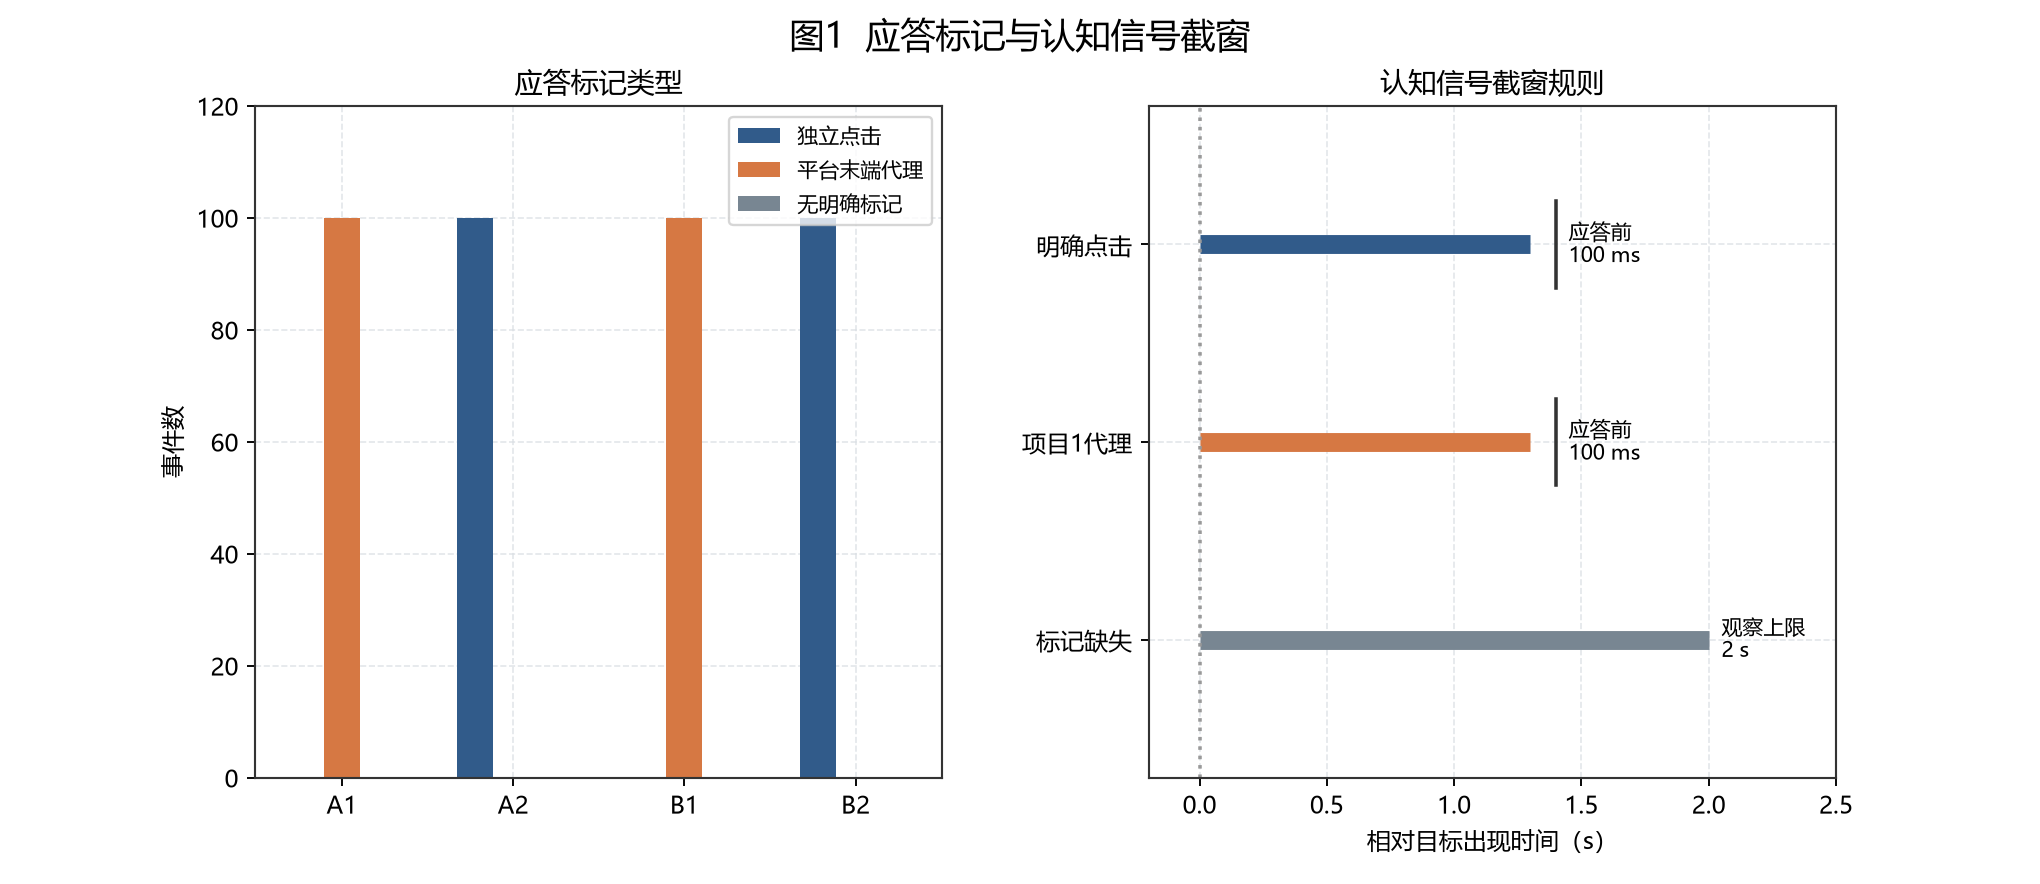
\includegraphics[width=0.94\textwidth]{q3_events.png}
\caption{四组记录的应答标记审计与认知信号截窗规则}
\label{fig:q3_events}
\end{figure}

\paragraph{（3）因果预处理与质量控制}

在每个连续时间块内，对原始 $F_z$、$F_3$、$F_4$ 依次施加 $60~\mathrm{Hz}$ 陷波和 $0.1$--$30~\mathrm{Hz}$ 四阶 Butterworth 带通。与问题一用于离线 ERP 对齐的双向滤波不同，本问采用单向因果滤波，使时刻 $t$ 的输出只依赖 $t$ 及其之前的样本，从而避免未来应答附近信号反向泄漏至较早认知阶段。每个试次以提示前 $[-250,0)~\mathrm{ms}$ 的中位数进行基线校正，并沿用硬件饱和、峰峰值和相邻采样跳变三类质量规则；阈值按变长窗口归一化后使用。

为比较不同阶段，定义编码、保持和提取三个不重叠时窗：
\begin{equation}
\mathcal W_i^{\mathrm E}=[t_i^{\mathrm c},t_i^{\mathrm c}+0.8),\qquad
\mathcal W_i^{\mathrm M}=[t_i^{\mathrm c}+0.8,t_i^{\mathrm T}),\qquad
\mathcal W_i^{\mathrm R}=[t_i^{\mathrm T},T_i^{\mathrm{end}}].
\tag{3-2}
\label{eq:q3_stages}
\end{equation}
窗口外样本记为缺失，不通过时间伸缩把不同反应速度强行对齐。质量控制后 A1、A2、B1、B2 分别保留 65、68、64、71 个试次，共 268 个主 EEG 试次，为后续状态估计提供统一输入。

\subsubsection{视觉--记忆--认知宏观模型与脑电差异解释}

\paragraph{（1）提示与目标的视觉驱动构造}

问题二已给出左右三角形经形状编码、LGN 中继和三级 E/I 神经群传播后的末级视觉源。为避免将真实点击方向写入模型，本文只利用提示符号 $d_i\in\{-1,+1\}$ 构造提示的共同分量 $v_i^{\mathrm c}(t)$ 与镜像差分分量 $v_i^{\Delta}(t)$，并为候选目标设置与点击方向无关的共同输入 $v_i^{\mathrm T}(t)$：
\begin{equation}
\boldsymbol v_i(t)=
\begin{bmatrix}
v_i^{\mathrm c}(t)\\ d_i v_i^{\Delta}(t)\\ v_i^{\mathrm T}(t-t_i^{\mathrm T})
\end{bmatrix}.
\tag{3-3}
\label{eq:q3_visual_input}
\end{equation}
其中，前两项继承问题二形状选择性网络的共同/反对称输出，第三项由统一目标脉冲经相同视觉动力学产生。由此，目标出现时刻可以触发认知提取，但真实应答、点击侧和正误标签均不进入视觉源。

\paragraph{（2）提示保持与目标触发提取}

设 $\boldsymbol m_i(t)\in\mathbb R^2$ 为提示保持状态，$\boldsymbol p_i(t)=[p_i^{\mathrm c}(t),p_i^{\Delta}(t),p_i^{\mathrm T}(t)]^{\mathsf T}$ 为认知整合状态。提示信息以时间常数 $\tau_m$ 衰减，目标到达后通过门函数 $G_i^{\mathrm T}(t)=\mathbf 1(t\ge t_i^{\mathrm T})$ 触发延迟提取；独立目标通路不写入提示记忆。其动力学方程为
\begin{equation}
\tau_m\dot{\boldsymbol m}_i(t)
=-\boldsymbol m_i(t)+
\begin{bmatrix}v_i^{\mathrm c}(t)\\ d_i v_i^{\Delta}(t)\end{bmatrix},
\tag{3-4}
\label{eq:q3_memory}
\end{equation}
\begin{equation}
\begin{aligned}
\tau_p\dot{p}_i^{\mathrm c}(t)
&=-p_i^{\mathrm c}(t)+v_i^{\mathrm c}(t)+G_i^{\mathrm T}(t)m_i^{\mathrm c}(t-\delta),\\
\tau_p\dot{p}_i^{\Delta}(t)
&=-p_i^{\Delta}(t)+d_i v_i^{\Delta}(t)+G_i^{\mathrm T}(t)m_i^{\Delta}(t-\delta),\\
\tau_p\dot{p}_i^{\mathrm T}(t)
&=-p_i^{\mathrm T}(t)+v_i^{\mathrm T}(t-t_i^{\mathrm T}),
\end{aligned}
\qquad \delta=50~\mathrm{ms}.
\tag{3-5}
\label{eq:q3_cognition}
\end{equation}
式~\eqref{eq:q3_memory}--\eqref{eq:q3_cognition} 将认知过程划分为“提示编码---缓慢保持---目标触发提取”三个环节。$\boldsymbol m_i$ 表示功能性的保持变量，$\boldsymbol p_i$ 表示多通路整合后的宏观群体状态；二者可用于构造可检验的头皮电位预测，但在缺少个体 MRI、深部电极与高密度导联时，不把 $\boldsymbol m_i$ 唯一归因于海马体活动。

\paragraph{（3）状态离散化与因果更新}

模型按原始采样率 $f_s=256~\mathrm{Hz}$ 在固定时间网格上积分，时间步长为 $\Delta t=1/f_s$。对任一一阶状态 $\tau_q\dot{\boldsymbol q}=-\boldsymbol q+\boldsymbol u$，采用指数 Euler 更新
\[
\boldsymbol q[n]=a_q\boldsymbol q[n-1]+(1-a_q)\boldsymbol u[n-1],
\qquad a_q=\exp\!\left(-\frac{\Delta t}{\tau_q}\right).
\]
由于第 $n$ 个状态只读取第 $n-1$ 个及更早输入，该离散形式保持因果性。$50~\mathrm{ms}$ 提取延迟约为 12.8 个采样间隔，计算时在记忆轨迹上进行线性分数延迟插值，而不简单取整为 13 个点，从而减少采样量化对目标触发时刻的影响。对每组记录，提示共同分量、提示差分分量和目标共同分量均先在统一时间轴上生成，再按该试次的 $t_i^{\mathrm T}$ 启动门函数；因此不同反应时只改变可评分终点，不改变目标前状态的计算结果。

从参数作用看，$\tau_m$ 决定提示信息跨越保持期的衰减速度，$\tau_p$ 决定目标后认知整合的响应速度，$T_{\mathrm T}$ 控制目标输入的持续范围，$\delta$ 则描述提取通路的固定传播延迟。四类参数分别影响波形的长期幅度、上升速度、驱动宽度和相位位置，具有相对清晰的结构分工；但在仅有三个额区通道时仍可能存在相关性，因此本文通过训练块内网格选择、岭惩罚和半合成参数恢复共同约束，而不把单次最小误差对应值直接视为生理真值。

\paragraph{（4）头皮观测映射与参数估计}

将式~\eqref{eq:q3_visual_input}--\eqref{eq:q3_cognition} 的状态拼接为设计矩阵 $\boldsymbol H_i(t;\boldsymbol\theta)$，经与实测 EEG 相同的因果滤波后，建立三通道有效观测模型
\begin{equation}
\widehat{\boldsymbol x}_i(t)=\boldsymbol H_i(t;\boldsymbol\theta)\boldsymbol B,
\qquad \widehat{\boldsymbol x}_i(t)\in\mathbb R^3,
\tag{3-6}
\label{eq:q3_observation}
\end{equation}
其中，$\boldsymbol\theta=(\tau_m,\tau_p,T_{\mathrm T},\delta)$ 为动力学参数，$\boldsymbol B$ 为从视觉、记忆与认知状态到 $F_z$、$F_3$、$F_4$ 的有效读出矩阵。同一外折内所有训练试次及左右提示共享 $\boldsymbol B$，只允许事件时刻和提示方向改变设计矩阵，因而测试波形不能依靠逐试次自由系数进行拟合。

考虑长时程脑电中还存在与任务无关的缓慢漂移，本文另设提示前背景辅助项。对每个通道，分别在三个提示前时间尺度上估计斜率 $s_{i,h,c}^{\mathrm{pre}}$，并将其因果外推为
\[
c_{i,h,c}(t)=s_{i,h,c}^{\mathrm{pre}}\tau_h
\left(1-\mathrm e^{-t/\tau_h}\right),
\qquad \tau_h\in\{0.25,1,4\}~\mathrm{s}.
\]
该项只使用提示出现前的样本，既不会读取测试试次未来脑电，也不改变式~\eqref{eq:q3_memory}--\eqref{eq:q3_cognition} 的认知状态。纯刺激模型以 $\boldsymbol H_i$ 为输入；背景辅助设置则将 $\boldsymbol c_i$ 追加到设计矩阵后单独拟合和报告。两者信息集合不同，前者用于机制比较，后者用于评估实际长窗预测中背景条件的价值。

为使编码、保持和提取三个阶段在变长试次中具有相同权重，令 $w_i(t)$ 在每个非空阶段内归一化。训练块上的稳健估计写为
\begin{equation}
(\widehat{\boldsymbol\theta},\widehat{\boldsymbol B})
=\arg\min_{\boldsymbol\theta,\boldsymbol B}
\sum_{i\in\mathcal T}\sum_t w_i(t)
\rho_{1.5}\!\left(
\frac{\boldsymbol x_i(t)-\boldsymbol H_i(t;\boldsymbol\theta)\boldsymbol B}
{\boldsymbol s_{\mathcal T}}
\right)
+\lambda\|\boldsymbol P\boldsymbol B\|_F^2,
\tag{3-7}
\label{eq:q3_fit}
\end{equation}
式中，$\rho_{1.5}(\cdot)$ 为逐通道作用的 Huber 损失，$\boldsymbol s_{\mathcal T}$ 为训练块尺度，$\boldsymbol P$ 对方向相关状态施加较强收缩，$\lambda$ 为岭惩罚系数。具体求解分为两个阶段：先对全部候选参数与 $\lambda$ 组合计算训练块内嵌套岭回归误差，筛出排名最靠前的两个组合；再对这两个组合逐折执行 Huber 迭代加权最小二乘，并按平均稳健损失确定最终参数。最后仅用四个外层训练块重估 $\boldsymbol B$，直接预测未参与任何选择的第五块。该“全网格筛选---稳健复核---外层预测”策略兼顾计算效率与异常样本抵抗能力。主要候选范围如表~\ref{tab:q3_parameters} 所示。

\begin{table}[H]
\centering
\caption{认知模型与决策层的主要参数}
\label{tab:q3_parameters}
\begin{tabular}{cllc}
\toprule
\textbf{参数} & \textbf{含义} & \textbf{候选值或设定} & \textbf{确定方式} \\
\midrule
$\tau_m$ & 提示保持时间常数 & $\{0.5,1,2,4\}~\mathrm{s}$ & 训练块内选择 \\
$\tau_p$ & 认知整合时间常数 & $\{0.1,0.3,0.6\}~\mathrm{s}$ & 训练块内选择 \\
$T_{\mathrm T}$ & 目标输入持续时间 & $\{0.1,0.2,0.4\}~\mathrm{s}$ & 训练块内选择 \\
$\delta$ & 提取延迟 & $0.05~\mathrm{s}$ & 固定设定 \\
$r_d$ & 方向状态收缩倍数 & $\{1,10\}$ & 训练块内选择 \\
$\lambda$ & 岭惩罚强度 & $\{10^{-3},10^{-2},10^{-1},1,10\}$ & 嵌套验证 \\
$\gamma$ & 决策证据增益 & 1.5 & 参考仿真设定 \\
$\sigma$ & 扩散噪声强度 & 0.6 & 参考仿真设定 \\
$b$ & 决策边界 & 1 & 归一化设定 \\
\bottomrule
\end{tabular}
\end{table}

\paragraph{（5）认知状态对脑电差异的解释}

左右提示的差异首先表现为 $d_i v_i^{\Delta}$ 的符号反转，随后在 $\tau_m$ 控制下形成不同方向的保持轨迹；目标到达时，门函数把延迟记忆状态重新注入 $p_i^{\Delta}$，经同一个观测矩阵投影为三导联差异。模型不为左右条件分别拟合两套参数，因此差异必须由提示的镜像输入及其随时间传播产生。为检查慢变背景的影响，另构造只使用提示前 EEG 斜率的背景辅助观测项，并与纯刺激输入模型分别报告。

图~\ref{fig:q3_eeg} 给出四组记录在 $F_z$ 通道上的留出平均预测。蓝线为式~\eqref{eq:q3_observation} 的刺激--认知模型，橙线在其信息集合之外加入严格提示前背景，黑线为实测脑电。背景辅助模型对长时间慢漂移的跟踪更充分，四组目标后均方误差相对纯刺激模型约下降 22\%--56\%；这一变化说明提示前背景对长窗预测具有价值，但不能据此把收益归因于记忆或海马机制。纯刺激模型则保留了更清晰的机制解释路径，用于后续记忆状态与慢趋势对照。

\begin{figure}[H]
\centering
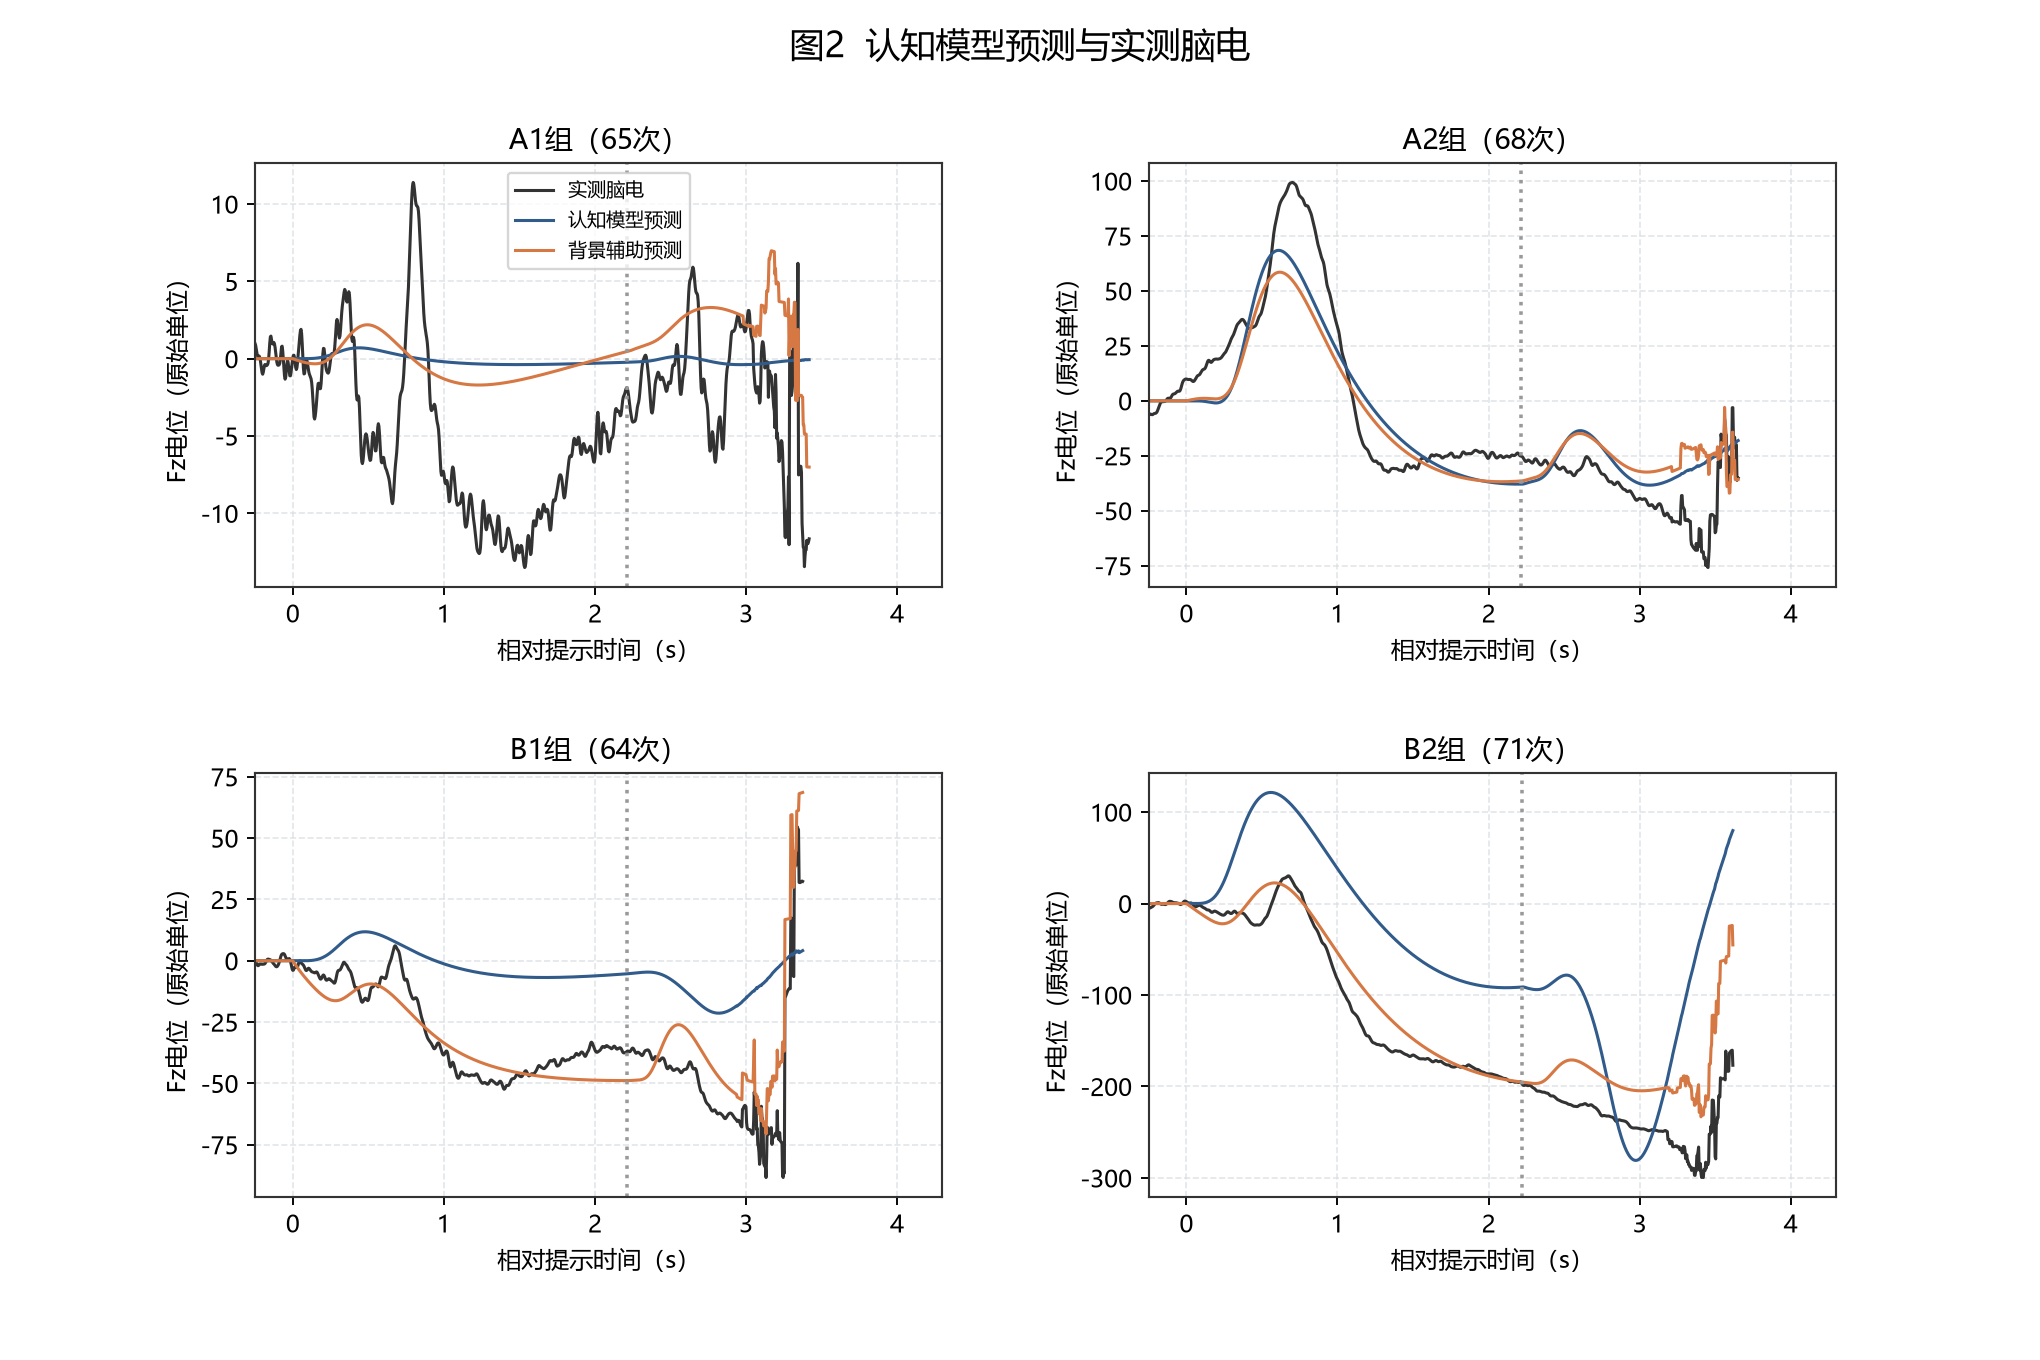
\includegraphics[width=0.72\textwidth]{q3_eeg.png}
\caption{四组记录的认知模型留出预测与实测 $F_z$ 脑电对比}
\label{fig:q3_eeg}
\end{figure}

\subsubsection{认知状态驱动的三类应答模型}

\paragraph{（1）认知证据与目标匹配}

取未经过头皮观测滤波的认知差分状态 $p_i^{\Delta}(t)$，以参考状态最大幅度 $a$ 归一化，并按提示方向对齐：
\begin{equation}
e_i(t)=\frac{d_i p_i^{\Delta}(t)}{a},
\qquad
a=\max_t\left|p_{\mathrm{ref}}^{\Delta}(t)\right|.
\tag{3-8}
\label{eq:q3_evidence}
\end{equation}
为使提示记忆能够与左右候选目标相比较，进一步复用问题二的形状编码。设归一化提示特征为 $\boldsymbol f_i^{\mathrm c}$，模拟布局中左、右目标特征为 $\boldsymbol f_i^{\mathrm L}$ 与 $\boldsymbol f_i^{\mathrm R}$，则方向匹配系数取为
\[
r_i=\frac{\langle\boldsymbol f_i^{\mathrm c},\boldsymbol f_i^{\mathrm R}\rangle
-\langle\boldsymbol f_i^{\mathrm c},\boldsymbol f_i^{\mathrm L}\rangle}{\kappa},
\]
其中，$\kappa$ 由左右标准形状的余弦距离归一化，使交换左右目标位置时 $r_i$ 符号反转。在主机制扰动实验中，为单独考察记忆保持、证据增益与噪声的作用，取 $r_i=s_i^*$；在目标匹配扩展中则由上式计算 $r_i$。正确目标侧 $s_i^*\in\{-1,+1\}$ 仅由平衡的模拟任务布局给定并用于结局评分，不由真实 MAT 文件中的点击方向反推，也不进入形状相似度计算。

决策变量 $z_i(t)$ 服从有界随机累积方程
\begin{equation}
\mathrm dz_i(t)=r_i\gamma e_i(t)\,\mathrm dt+\sigma\,\mathrm dW_i(t),
\qquad z_i(0)=0,\qquad |z_i(t)|<b,
\tag{3-9}
\label{eq:q3_diffusion}
\end{equation}
其中，$\gamma$ 为证据增益，$\sigma$ 为扩散噪声，$W_i(t)$ 为标准 Wiener 过程，$b$ 为对称决策边界。$z_i$ 只读取认知证据，不作为新的头皮源，也不反馈修改 $\boldsymbol m_i$ 或 $\boldsymbol p_i$；模型未单独估计感觉--运动转换和按键执行耗时，因此首次越界时间表示模型决策时间，而不直接等同于实测点击间隔。图~\ref{fig:q3_states} 展示基准、短保持和关闭提取三种情况下的记忆状态、认知状态与决策驱动。缩短 $\tau_m$ 会使目标出现前的可用证据衰减；关闭提取则使目标后差分状态接近零，从机制上给出迟疑或错误应答的形成路径。

\begin{figure}[H]
\centering
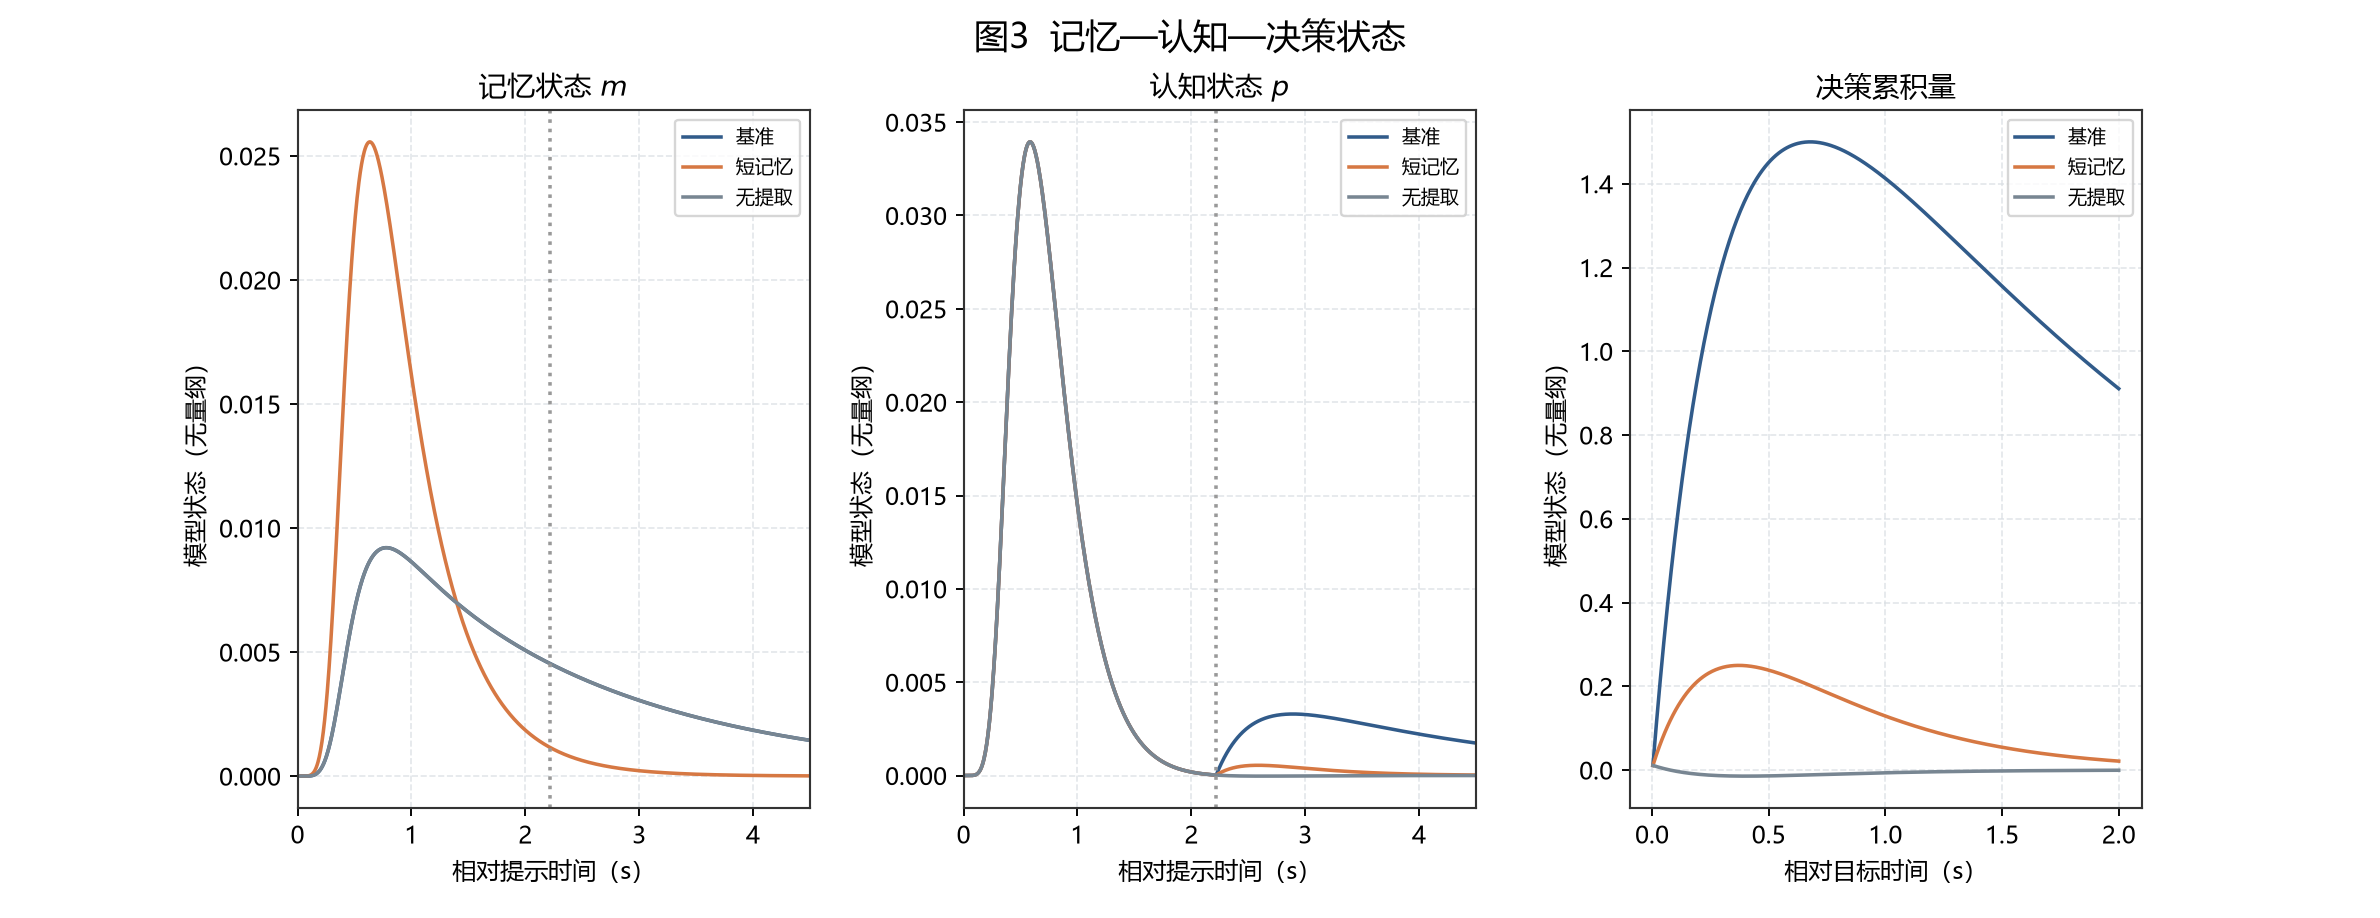
\includegraphics[width=0.96\textwidth]{q3_states.png}
\caption{提示保持、目标触发认知状态与决策证据的连续演化}
\label{fig:q3_states}
\end{figure}

\paragraph{（2）正确、错误与未决结局的统一判定}

令 $T_i=\inf\{t:|z_i(t)|\ge b\}$ 为首次越界时间，仿真截止时刻为 $D$。若 $T_i\le D$，则 $\operatorname{sign}[z_i(T_i)]$ 给出选择；若截止前未越界，则该轨迹记为未决并在 $D$ 处右删失。三类结果定义为
\begin{equation}
Y_i=
\begin{cases}
\text{正确}, & T_i\le D,\ \operatorname{sign}[z_i(T_i)]=s_i^*,\\
\text{错误}, & T_i\le D,\ \operatorname{sign}[z_i(T_i)]\ne s_i^*,\\
\text{未决}, & T_i>D.
\end{cases}
\tag{3-10}
\label{eq:q3_outcome}
\end{equation}
在任意时刻 $t$，分别记正确越界、错误越界的累计概率为 $F_{\mathrm c}(t)$、$F_{\mathrm e}(t)$，未决概率为 $S_{\mathrm u}(t)$，则模型逐时满足
\[
F_{\mathrm c}(t)+F_{\mathrm e}(t)+S_{\mathrm u}(t)=1.
\]
这一守恒关系保证错误轨迹不会被剔除，未决轨迹也不会被强制归入错误。数值实现采用 $\Delta t=1/256~\mathrm{s}$ 的首次越界判定，一旦轨迹触及边界便停止更新其选择和决策时间；不同机制场景使用共同随机数，使比例变化主要反映被扰动参数而非蒙特卡洛样本差异。

未决轨迹只保存观察时长 $D$，不把 $D$ 或 0 伪装成反应时间。对实测项目二点击，采用同样的右删失定义计算任意点击的描述性生存曲线：若时刻 $u_j$ 的风险集为 $n_j$、点击数为 $d_j$，则
\begin{equation}
\widehat S(t)=\prod_{u_j\le t}\left(1-\frac{d_j}{n_j}\right).
\tag{3-11}
\label{eq:q3_survival}
\end{equation}
该曲线反映“截至时刻 $t$ 尚未出现点击”的比例，但不区分点击是否正确，也不把项目一平台末端代理当作真实点击事件。

\paragraph{（3）机制扰动与三类决策仿真}

在参考设置 $\tau_m=2~\mathrm{s}$、$\tau_p=0.3~\mathrm{s}$、$\gamma=1.5$、$\sigma=0.6$、$b=1$、$D=2~\mathrm{s}$ 下，对每个场景生成 6000 条轨迹，并使用相同随机数实施单因素比较。表~\ref{tab:q3_decision} 与图~\ref{fig:q3_decision} 给出结果。基准场景的证据持续且噪声适中，轨迹大多在正确边界越界；短保持、关闭提取和低证据增益均提高未决比例；高噪声主要增加错误越界；缩短截止时间则在基本不改变早期错误率的同时增加行政未决比例。上述结果说明同一认知状态模型能够生成题目要求考虑的多种应答情形。

\begin{table}[H]
\centering
\caption{不同机制扰动下的三类决策仿真结果}
\label{tab:q3_decision}
\resizebox{\textwidth}{!}{%
\begin{tabular}{lccccc}
\toprule
\textbf{场景} & \textbf{轨迹数} & \textbf{正确比例} & \textbf{错误比例} & \textbf{未决比例} & \textbf{受限平均时间/s} \\
\midrule
基准 & 6000 & 0.9742 & 0.0010 & 0.0248 & 0.8665 \\
短保持 & 6000 & 0.3315 & 0.1405 & 0.5280 & 1.6000 \\
关闭提取 & 6000 & 0.2150 & 0.2310 & 0.5540 & 1.6305 \\
高噪声 & 6000 & 0.7737 & 0.2128 & 0.0135 & 0.5612 \\
低证据增益 & 6000 & 0.3072 & 0.1563 & 0.5365 & 1.6161 \\
短仿真截止 & 6000 & 0.8300 & 0.0010 & 0.1690 & 0.8095 \\
\bottomrule
\end{tabular}}
\end{table}

\begin{figure}[H]
\centering
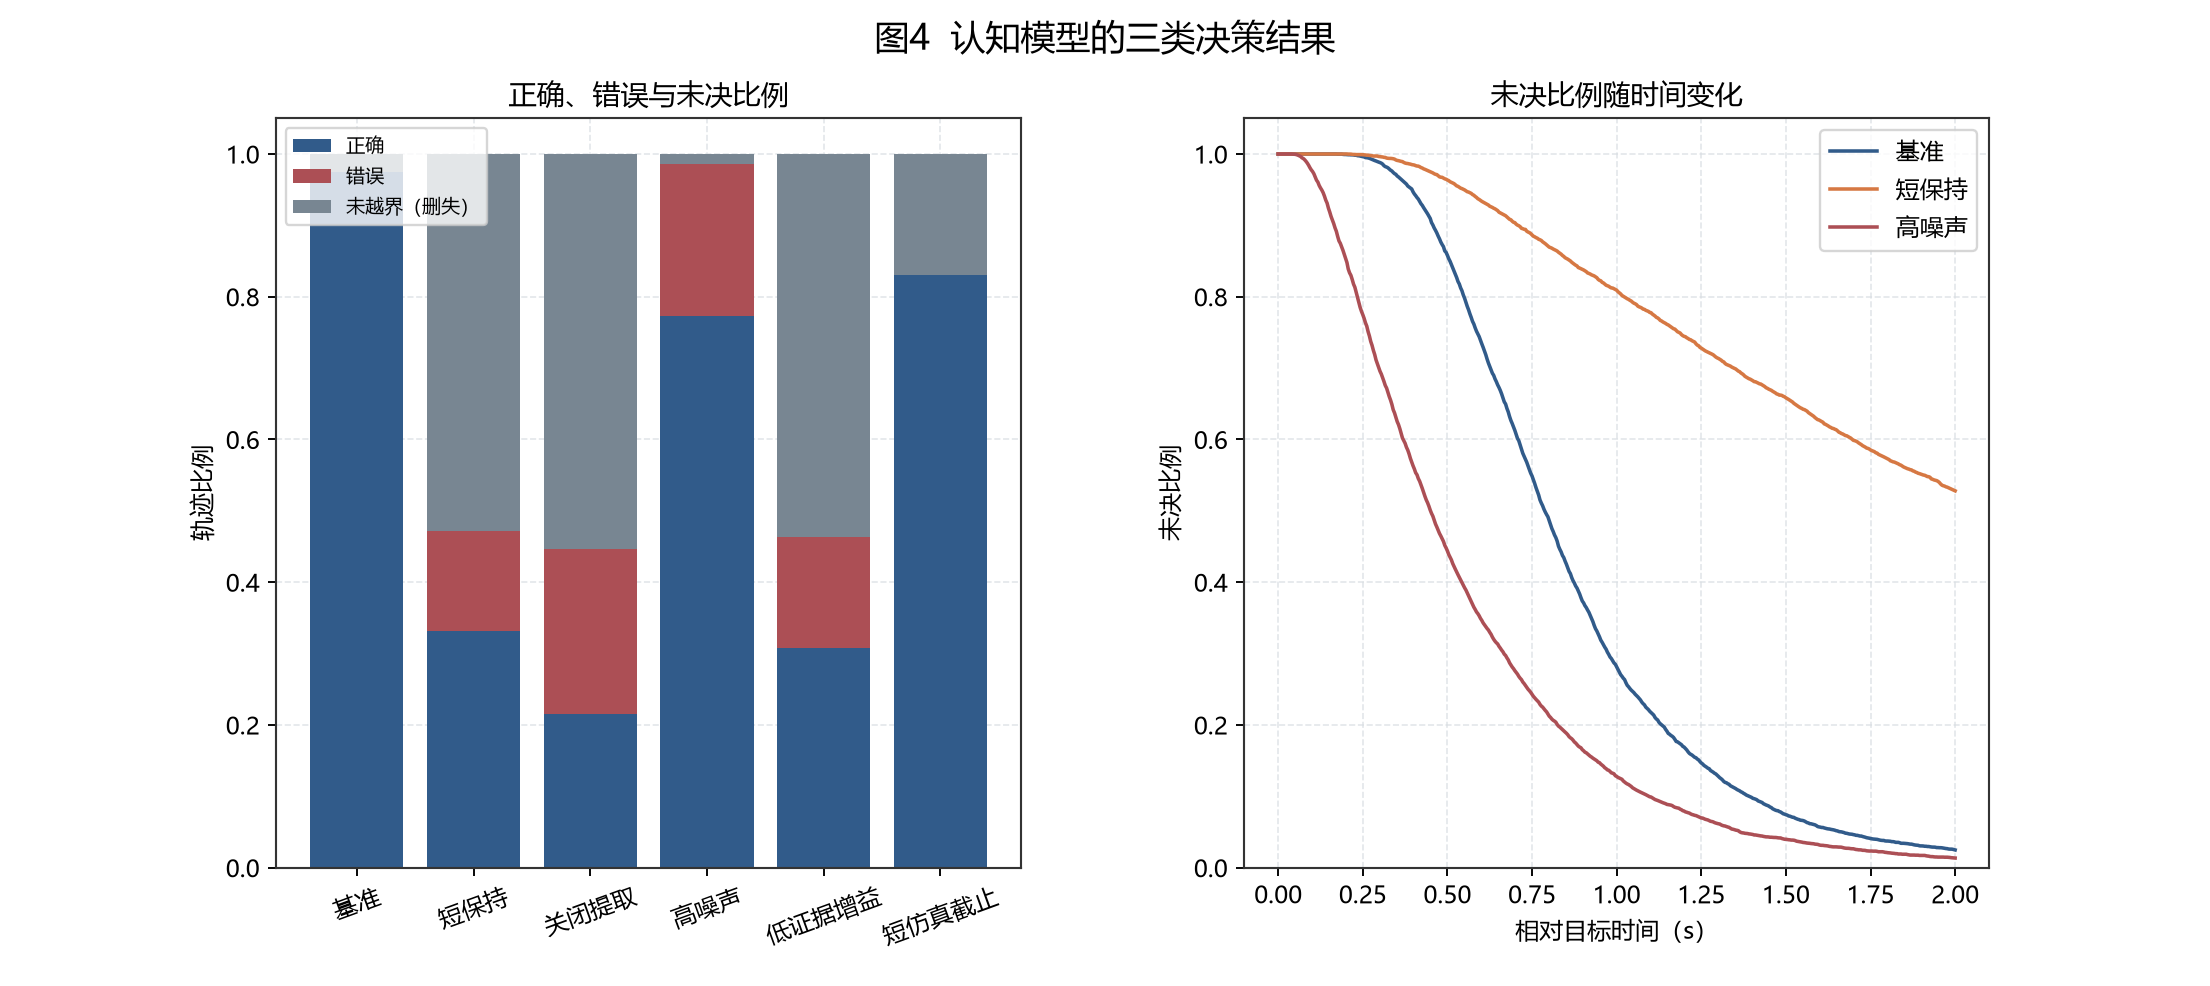
\includegraphics[width=0.95\textwidth]{q3_decision.png}
\caption{认知状态驱动的正确、错误与未决决策仿真}
\label{fig:q3_decision}
\end{figure}

表~\ref{tab:q3_decision} 中的比例是给定模拟目标布局和参数下的模型输出，Wilson 区间只反映蒙特卡洛抽样误差，不是受试者总体置信区间。由于原始数据未提供正确目标映射和正式超时规则，本文不将其解释为两名受试者的实测正确率或超时率；其作用是验证模型结构能够以统一方程表示正确、错误和未决三种可能结局。

\subsubsection{模型求解结果与验证}

\paragraph{（1）连续时间块外层留出验证}

对每个外层测试块，使用训练块确定的参数和读出矩阵重建三通道 EEG。令 $\mathcal I_{g,c}$ 表示阶段 $g$、通道 $c$ 的有效测试样本集合，则阶段均方误差为
\begin{equation}
\mathrm{MSE}_{g}=\frac{1}{3}\sum_{c=1}^{3}
\frac{1}{|\mathcal I_{g,c}|}
\sum_{(i,t)\in\mathcal I_{g,c}}
\left[x_{i,c}(t)-\widehat x_{i,c}(t)\right]^2.
\tag{3-12}
\label{eq:q3_mse}
\end{equation}
为判断目标后记忆--认知结构是否优于一般慢变化，设置不含提示记忆、仅使用平滑慢趋势基函数的 N3 对照，并定义相对预测增益
\begin{equation}
S_g=1-\frac{\mathrm{MSE}_{g}^{\mathrm{N2}}}
{\mathrm{MSE}_{g}^{\mathrm{N3}}}.
\tag{3-13}
\label{eq:q3_gain}
\end{equation}
$S_g>0$ 表示认知模型在该阶段的留出误差更低。表~\ref{tab:q3_eeg_validation} 给出目标后提取阶段的结果，区间由 2000 次连续时间块重采样获得。A1、A2、B1 的点估计为正，B2 略为负；四组区间均跨越 0，说明现有三导联、两名受试者记录支持将该结构作为可计算的候选认知模型，但尚不足以把缓慢成分唯一解释为特定深部记忆源。

\begin{table}[H]
\centering
\caption{认知模型相对慢趋势对照的目标后留出预测增益}
\label{tab:q3_eeg_validation}
\begin{tabular}{ccccc}
\toprule
\textbf{记录} & \textbf{EEG 试次} & \textbf{$S_{\mathrm R}$} & \textbf{95\% 块重采样区间} & \textbf{结果方向} \\
\midrule
A1 & 65 & 0.0244 & $[-0.0134,\ 0.0742]$ & 正向 \\
A2 & 68 & 0.0022 & $[-0.0125,\ 0.0114]$ & 正向 \\
B1 & 64 & 0.0034 & $[-0.0028,\ 0.0163]$ & 正向 \\
B2 & 71 & $-0.0148$ & $[-0.0547,\ 0.0298]$ & 轻微负向 \\
\bottomrule
\end{tabular}
\end{table}

\paragraph{（2）观察窗与点击时间敏感性}

将目标后行政观察上限分别设为 1.5、2.0 与 $2.5~\mathrm{s}$，使用同一组冻结参数，并仅在各上限共同保留的试次上重新评分。由图~\ref{fig:q3_window} 左侧可知，四组 $S_{\mathrm R}$ 的点估计随观察上限基本稳定，结论不依赖单一 $2~\mathrm{s}$ 设置；右侧给出 A2、B2 的实测任意点击时间，两组曲线均在约 $1.0~\mathrm{s}$ 后开始下降，并在 $2~\mathrm{s}$ 附近接近零。该结果只用于说明窗口覆盖了现有点击时间分布，点击间隔同时包含认知与运动过程，不能直接等同于模型决策时间。

\begin{figure}[H]
\centering
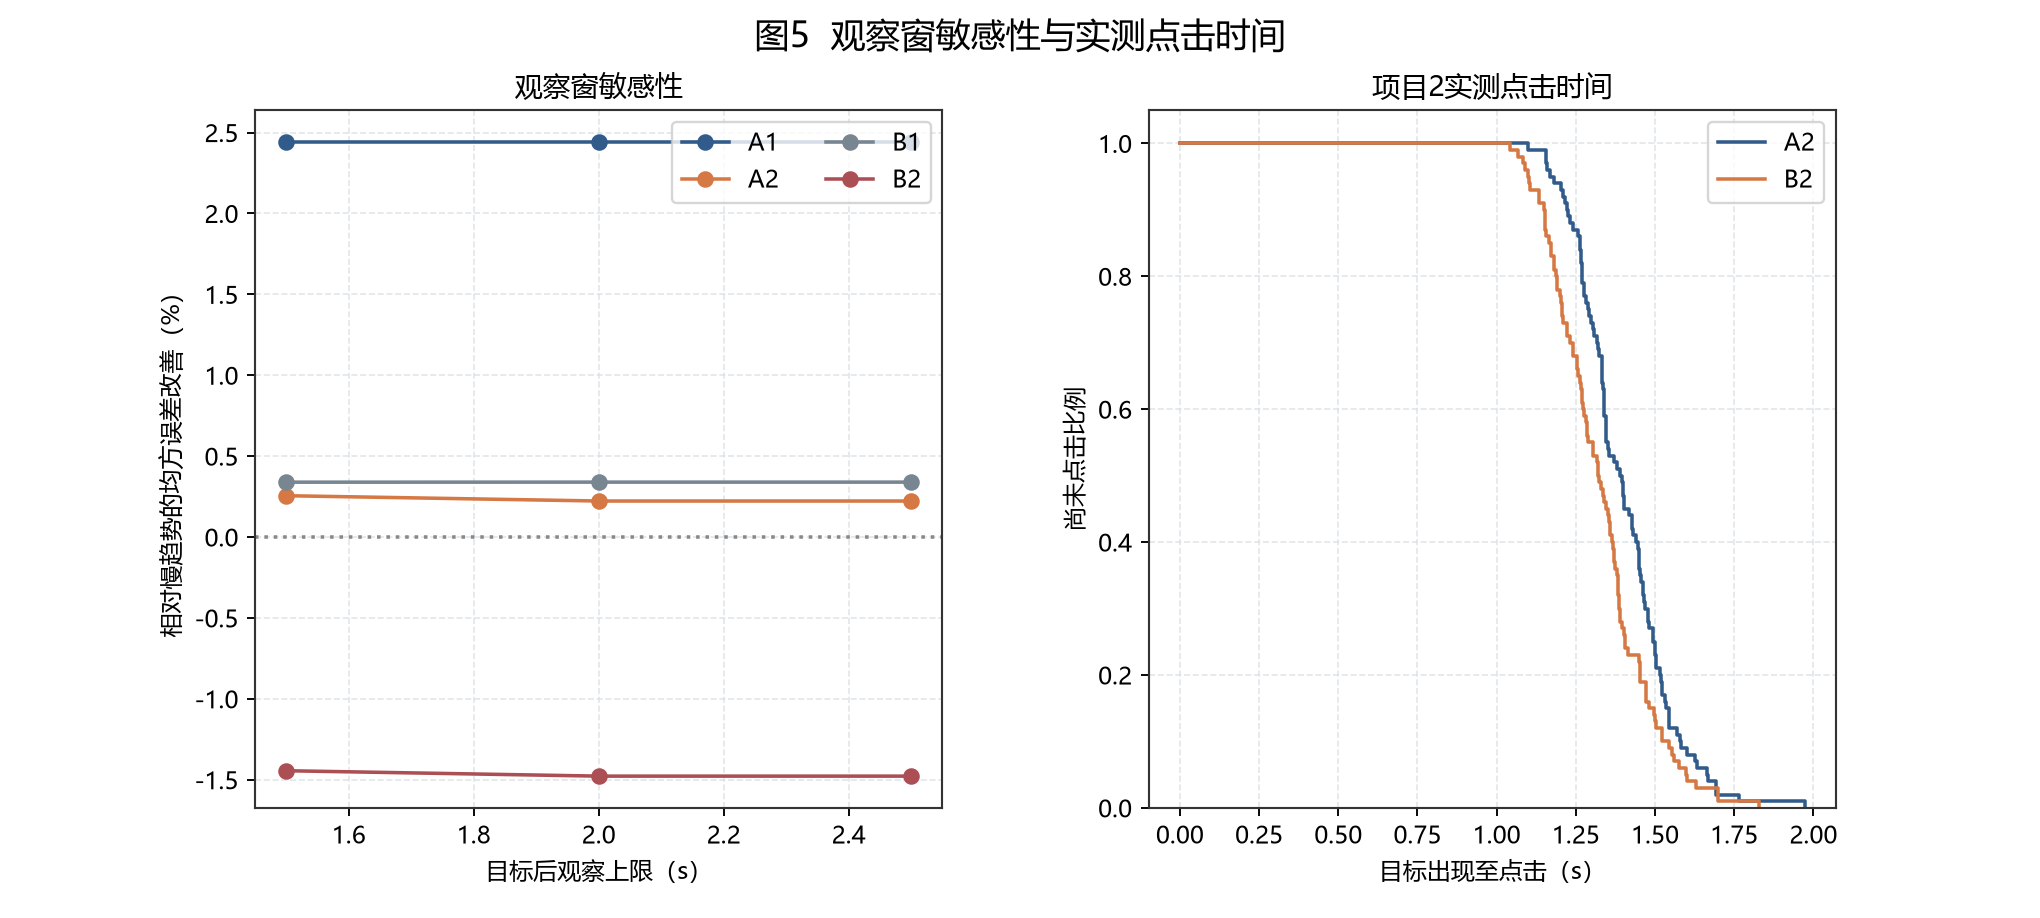
\includegraphics[width=0.80\textwidth]{q3_window.png}
\caption{目标后观察窗敏感性与项目二实测点击时间分布}
\label{fig:q3_window}
\end{figure}

\paragraph{（3）消融、参数恢复与数值审计}

除慢趋势对照外，本文分别关闭记忆向认知状态的投影、关闭目标触发提取，并改变 $\tau_m$、$\gamma$、$\sigma$ 和 $D$，检查结论是否由单一环节偶然造成。进一步将记忆时间常数搜索范围扩展至 $0.25$--$8~\mathrm{s}$，新拟合相对原参数网格未呈现稳定的外层误差改善，因而保留训练内选择的主结果。半合成参数恢复表明：无噪声时 9 个场景均能恢复生成时间常数；噪声为 0.5 倍时精确恢复率为 0.333，噪声为 1 倍时精确恢复率下降至 0。该结果说明求解程序在理想条件下可辨识，但真实噪声会显著增加时间常数的不确定性，故本文不对单个受试者报告唯一生理参数。

最终验证共通过 28 项自动测试，覆盖未来 EEG 不影响过去状态、外层测试块不参与参数估计、目标不写入提示记忆、缺失点击不等于超时、平台代理不进入真实生存曲线以及三类结局概率守恒等关键性质。独立审计重新计算 31356 条阶段误差记录，最大相对差异为 $3.17\times10^{-16}$；冻结预测重建的最大绝对差异为 0；36000 条决策轨迹在时间步长减半后，三类比例的最大绝对变化为 0.00375。上述结果验证了程序实现、数据隔离和数值计算的一致性。

综上，本文构建了由视觉编码、提示保持、目标触发提取、头皮观测与随机决策组成的认知宏观模型。该模型能够在同一框架下处理应答代理、独立点击和潜在的未决试次，并在连续时间块留出条件下生成可与实测 EEG 比较的预测波形。现有结果支持其作为视觉认知过程的功能性解释与仿真平台；对深部脑区来源、真实正误及实验超时的进一步确认，仍需结合逐试次目标布局、高密度 EEG 或独立深部观测数据。



%% -----------------------------------------------------------------------------
%% 模块 6：模型评价与优缺点讨论
%% -----------------------------------------------------------------------------
\section{模型优缺点评价}
\subsection{问题一模型评价}

\textbf{模型的优点：}该模型以垂直/水平分量、软门控和均值保护兼顾伪影抑制与响应保留，并通过五折留出和训练内半合成选型减少信息泄漏。四组代理 MAE 降幅为 $5.4\%$--$10.0\%$，左右差异保留率为 $0.813$--$0.952$；三次 B 样条可进一步给出连续响应曲线。

\textbf{模型的缺点：}数据缺少同步眼电、眼动和独立无噪声脑电，代理误差下降不能直接等同于真实神经信号恢复。四组 SNR 代理增量区间均跨越零点，弱扰动与部分时间分段下的收益仍有波动，现有结果主要适用于已知条件下的离线响应描述。

\textbf{改进思路：}增加眼电、眼动及中央、顶区、枕区电极，在独立受试者上固定参数验证；依据训练块信噪比自适应调节收缩强度，并用时延校准的因果滤波替代双向滤波。

\subsection{问题二模型评价}

\textbf{模型的优点：}模型构建了“形状编码--LGN 中继--三级 E/I 群体--突触源--头皮观测”的完整计算链，左右条件共享参数，并用消融检验结构贡献。连续时间块留出、1999 次块内置换和 maxT 校正将机制解释、差异预测与单试次判别分开评价，二十三维特征亦可用于未知试次。

\textbf{模型的缺点：}仅有 Fz、F3、F4 三个额区电极，缺少枕顶区、电眼和个体头模型，有效观测矩阵不能作为唯一神经源定位。简单幅值和机制特征的总体 BA 分别为 $0.5161$、$0.4471$，跨块方向信息较弱，稳定判别能力仍有提升空间。

\textbf{改进思路：}增加高密度 EEG、同步眼动和个体 MRI，将共同背景与方向差异分别正则化；固定时间窗与候选特征，并在扩大受试者规模后检验跨个体稳定性。

\subsection{问题三模型评价}

\textbf{模型的优点：}模型区分独立点击、平台代理和应答不可观测三类事件，按应答前约 $100~\mathrm{ms}$ 截取信号；并将视觉编码、提示保持、目标提取、头皮观测与随机决策统一起来，表示正确、错误和未决三类结局。时间块留出、窗口敏感性、消融和数值审计保证了过程可复核。

\textbf{模型的缺点：}数据缺少逐试次正确目标、完整布局和正式超时阈值，三类决策比例只能作为机制仿真结果。三导联 EEG 不能直接定位海马体等深部来源；相对慢趋势对照的四组区间均覆盖零点，且时间常数恢复精度随噪声增加而下降。

\textbf{改进思路：}完整记录目标布局、正误、超时和动作触发信息，增加高密度 EEG、眼电与独立深部观测；采用分层状态空间模型区分认知决策和运动时间，并在新增受试者上检验泛化能力。
% ==============================================================================
% 参考文献（GB/T 7714 国标学术规范，支持点击超链接跳转）
% ==============================================================================


\clearpage
\begin{thebibliography}{99}
\addcontentsline{toc}{section}{参考文献} % 将参考文献加入到 PDF 目录大纲中
\bibitem{glomb2022computational}
GLOMB K, CABRAL J, CATTANI A, et al. Computational models in electroencephalography[J]. \emph{Brain Topography}, 2022, 35(2): 142--161.
\bibitem{wilson1972excitatory}
WILSON H R, COWAN J D. Excitatory and inhibitory interactions in localized populations of model neurons[J]. \emph{Biophysical Journal}, 1972, 12(1): 1--24.
\bibitem{steeghs2025slow}
STEEGHS-TURCHINA M, SRINIVASAN R, NUNEZ P L, et al. Slow wave dynamics of scalp EEG can be explained by simple statistical models of long-range connections[J]. \emph{NeuroImage}, 2025, 321: 121418.
\bibitem{daume2024control}
DAUME J, KAMINSKI J, et al. Control of working memory by phase-amplitude coupling of human hippocampal neurons[J]. \emph{Nature}, 2024, 629: 808--816.
\bibitem{acebron2005kuramoto}
ACEBR\'{O}N J A, BONILLA L L, P\'{E}REZ VICENTE C J, et al. The Kuramoto model: A simple paradigm for synchronization phenomena[J]. \emph{Reviews of Modern Physics}, 2005, 77(1): 137--185.
\bibitem{azzopardi2014ventral}
AZZOPARDI G, PETKOV N. Ventral-stream-like shape representation: from pixel intensity values to trainable object-selective COSFIRE models[J]. \emph{Frontiers in Computational Neuroscience}, 2014, 8: 112.
\end{thebibliography}

\appendix
% ==============================================================================
% 附录：核心算法程序代码（严格对标华为杯优秀论文版式）
% ==============================================================================
\clearpage
\begin{center}
    {\zihao{3} \heiti \textbf{附\quad 录}}
\end{center}
\addcontentsline{toc}{section}{附录}

\noindent
% 1. 表头部分：注意第二行末尾不要加 \hline，让下方代码框的顶线无缝接上！
\begin{tabularx}{\linewidth}{|p{0.55\textwidth}|>{\centering\arraybackslash}X|}
\hline
\multicolumn{2}{|l|}{\textbf{附录 1} 由于篇幅问题对附录中的代码进行了删减，完整代码在对应的附件中} \\
\hline
\centering 问题一建模代码 & 编程语言：Python \\ 
\end{tabularx}%
\vspace{1.2pt}% 消除微小缝隙，使竖线严丝合缝对接

% 2. 代码部分：封闭单框，彻底关闭行号，左右边距设为 0
\begin{lstlisting}[
    frame=single,
    numbers=none,           % 核心：关闭行号，彻底去掉左侧数字！
    xleftmargin=3.4pt,        % 左侧零边距，与表格左边框精准对齐
    xrightmargin=3.4pt,       % 右侧零边距，与表格右边框精准对齐
    basicstyle=\footnotesize\ttfamily
]
import os
import argparse
import hashlib
import json
import platform
from pathlib import Path

import numpy as np
import pandas as pd
from scipy.interpolate import LSQUnivariateSpline
import scipy.io as sio
from scipy.stats import median_abs_deviation
from scipy.signal import find_peaks, butter, sosfiltfilt, iirnotch, filtfilt, savgol_filter, welch
import matplotlib
matplotlib.use('Agg')
import matplotlib.pyplot as plt
from sklearn.model_selection import StratifiedKFold, train_test_split

ROOT = Path(__file__).resolve().parent

# 时间轴、校正参数和绘图设置
FS_EXPECTED = 256
PRE_SEC = 0.25      # 刺激前 250 ms 基线
POST_SEC = 0.80     # 刺激后 800 ms 分析窗

N_PRE = round(PRE_SEC * FS_EXPECTED)
N_POST = round(POST_SEC * FS_EXPECTED)
TIMES = np.arange(-N_PRE, N_POST) / FS_EXPECTED
TIMES_MS = TIMES * 1000.0

P300_MASK = (TIMES >= 0.25) & (TIMES <= 0.50)
CHANNEL_NAMES = ["Fz", "F3", "F4"]

# 双分量校正参数
CORRECTION_PARAMS = {
    "win_blink": 41,        # 垂直眼电平滑窗长 (约 160 ms)
    "win_saccade": 31,      # 水平扫视平滑窗长 (约 120 ms)
    "gate_z_v": 2.2,        # 垂直软门控阈值
    "gate_z_h": 2.2,        # 水平软门控阈值
    "gate_width": 1.2,      # 软门控过渡带宽度
    "reg_lambda": 0.05,     # 岭回归正则化系数，防止过减
    "max_beta_v": 1.8,      # 垂直通道最大增益
    "max_beta_h": 1.5,      # 水平通道最大增益
}

def load_mat_file(filepath):
    """读取赛题 .mat 文件"""
    mat = sio.loadmat(filepath, squeeze_me=True, struct_as_record=False)
    fs = int(mat["SampleRate"])
    labels = list(mat["DataLabel"])
    data = mat["data"]
    return fs, labels, data

def extract_viscue_events(viscue):
    """根据 VisCue 通道提取事件上升沿与方向标签 (-1: 左三角, +1: 右三角)"""
    nonzero = (viscue != 0)
    onset_mask = nonzero & np.r_[True, ~nonzero[:-1]]
    onsets = np.where(onset_mask)[0]
    cue_values = viscue[onsets].astype(int)
    return onsets, cue_values

def segment_epochs(signal, onsets, n_pre=N_PRE, n_post=N_POST):
    """截取 [-N_PRE, N_POST] 试次片段，shape: (trials, channels, time)"""
    epochs = []
    n_samples = signal.shape[-1]
    for onset in onsets:
        start = onset - n_pre
        end = onset + n_post
        if start < 0 or end > n_samples:
            continue
        epochs.append(signal[..., start:end])
    return np.stack(epochs, axis=0)

def preprocess_continuous_eeg(data_3ch, fs=FS_EXPECTED):
    """
    对连续 3 通道 EEG 进行预处理：
    1. 60 Hz 陷波滤波（抑制实测强工频干扰）
    2. 0.1-30 Hz 四阶 Butterworth 零相位带通
    """
    b_notch, a_notch = iirnotch(w0=60.0, Q=30.0, fs=fs)
    notched = filtfilt(b_notch, a_notch, data_3ch, axis=-1)

    sos = butter(4, [0.1, 30.0], btype="bandpass", fs=fs, output="sos")
    filtered = sosfiltfilt(sos, notched, axis=-1)
    return filtered

def robust_baseline_correct(epochs, n_pre=N_PRE):
    """使用刺激前 [-250, 0] ms 的稳健中位数/截断均值作为基线，扣除慢漂移偏置"""
    baseline = np.median(epochs[:, :, :n_pre], axis=2, keepdims=True)
    return epochs - baseline

def detect_bad_trials(raw_epochs, filtered_epochs):
    """
    识别不可恢复严重坏试次：
    1. 原始采样点发生 ±1000 硬件饱和截幅连续超过 15 个点
    2. 峰峰值超过 1800 原始幅值单位
    3. 相邻点发生物理不可能的跳跃
    """
    peak_to_peak = np.ptp(filtered_epochs, axis=2).max(axis=1)
    sat_points = np.sum(np.abs(raw_epochs) >= 999.0, axis=(1, 2))
    max_jump = np.max(np.abs(np.diff(filtered_epochs, axis=2)), axis=(1, 2))

    irrecoverable = (sat_points >= 15) | (peak_to_peak > 1800) | (max_jump > 600)
    return irrecoverable

def correct_single_epoch(epoch, template, scale_v, scale_h, params=CORRECTION_PARAMS):
    """双分量自适应校正核心算法"""
    residual = epoch - template

    # 1. 垂直与水平正交眼动参考
    ref_v = np.median(residual, axis=0)
    ref_v_smooth = savgol_filter(ref_v, window_length=params["win_blink"], polyorder=3)
    ref_h = 0.5 * (residual[2] - residual[1])
    ref_h_smooth = savgol_filter(ref_h, window_length=params["win_saccade"], polyorder=3)

    # 2. 动态自适应软门控
    z_v = np.abs(ref_v_smooth) / (scale_v + 1e-6)
    gate_v = np.clip((z_v - params["gate_z_v"]) / params["gate_width"], 0, 1)
    art_v = ref_v_smooth * gate_v

    z_h = np.abs(ref_h_smooth) / (scale_h + 1e-6)
    gate_h = np.clip((z_h - params["gate_z_h"]) / params["gate_width"], 0, 1)
    art_h = ref_h_smooth * gate_h

    # 3. 带约束岭回归消除
    X = np.column_stack([art_v, art_h])
    lambda_eye = params["reg_lambda"] * np.eye(2)
    XtX = X.T @ X + lambda_eye

    corrected = epoch.copy()
    for ch in range(3):
        y = residual[ch]
        beta = np.linalg.solve(XtX, X.T @ y)
        beta_v = float(np.clip(beta[0], 0, params["max_beta_v"]))
        beta_h = float(np.clip(beta[1], -params["max_beta_h"], params["max_beta_h"]))
        if ch == 0:
            beta_h = float(np.clip(beta_h, -0.3, 0.3))
        corrected[ch] = epoch[ch] - (beta_v * art_v + beta_h * art_h)

    corrected -= np.mean(corrected[:, :N_PRE], axis=1, keepdims=True)
    return corrected
\end{lstlisting}

% ==============================================================================
% 附录 2：问题二建模核心代码
% ==============================================================================

\clearpage

\noindent
% 1. 表头部分：注意第二行末尾不要加 \hline，让下方代码框的顶线无缝接上！
\begin{tabularx}{\linewidth}{|p{0.55\textwidth}|>{\centering\arraybackslash}X|}
\hline
\multicolumn{2}{|l|}{\textbf{附录 2} 由于篇幅问题对附录中的代码进行了删减，完整代码在对应的附件中} \\
\hline
\centering 问题二建模代码 & 编程语言：Python \\ 
\end{tabularx}%
\vspace{1.2pt}% 消除微小缝隙，使竖线严丝合缝对接

% 2. 代码部分：封闭单框，彻底关闭行号，左右边距设为 0
\begin{lstlisting}[
    frame=single,
    numbers=none,           % 核心：关闭行号，彻底去掉左侧数字！
    xleftmargin=3.4pt,        % 左侧零边距，与表格左边框精准对齐
    xrightmargin=3.4pt,       % 右侧零边距，与表格右边框精准对齐
    basicstyle=\footnotesize\ttfamily
]
import numpy as np
from scipy.integrate import solve_ivp
from scipy.optimize import root
from scipy.special import expit
from scipy.ndimage import maximum_filter

# ==================== 1. COSFIRE 几何边缘组合编码 ====================
def encode_shapes(left_img, right_img, templates):
    """
    基于 COSFIRE 空间边缘组合思想，提取三角形边缘与朝向偏好驱动
    """
    images = np.stack([left_img, right_img])
    # 空间定向边缘滤波响应 (Gabor 算子模拟初级视皮层感受野)
    response = np.stack([maximum_filter(oriented_edges(im), size=(1, 3, 3)) for im in images])
    
    # 局部特征空间容差模糊最大值与几何加权平均
    activation = np.array([[np.exp(np.mean(np.log([r[o, y, x] + 1e-5 
                           for y, x, o in pos]))) for pos in templates] 
                           for r in response])
    # 归一化为对偶形状输入向量
    activation /= np.maximum(np.diag(activation[:2]), 1e-10)[None, :]
    return activation  # 输出左、右对偶形状驱动强度

# ==================== 2. 三级 Wilson-Cowan 介观动力学网络 ====================
def simulate(inputs, scale=1.0, recurrence=0.1, duration=52/256):
    """
    三级 E/I 神经元群动力学仿真：LGN 中继 -> 早期视皮层 -> 形状整合 -> 前额响应
    """
    tau_e = scale * np.array([0.020, 0.040, 0.080])[:, None]
    tau_i = 2 * tau_e
    tau_se = scale * np.array([0.025, 0.050, 0.100])[:, None]
    tau_si = 3 * tau_se
    W = (np.ones((3, 3)) - np.eye(3)) / 2

    eq = root(lambda z: np.r_[-z[:3] + expit(z[:3]-z[3:] + recurrence*W@z[:3]-2),
                              -z[3:] + expit(z[:3]-z[3:]-2)], np.full(6, 0.12))
    resting_e = np.tile(eq.x[:3], (3, 1))
    resting_i = np.tile(eq.x[3:], (3, 1))
    state0 = np.r_[np.zeros(3), resting_e.ravel(), resting_i.ravel(), np.zeros(36)]

    def derivative(t, state, feature):
        g = state[:3]
        e = state[3:12].reshape(3, 3)
        i = state[12:21].reshape(3, 3)
        ue, ve, ui, vi = state[21:].reshape(4, 3, 3)
        
        drive = np.vstack([g, 3 * (e[:-1] - resting_e[:-1])])
        de = (-e + expit(e - i + recurrence * (e @ W.T) + drive - 2)) / tau_e
        di = (-i + expit(e - i - 2)) / tau_i
        
        stim_drive = 3 * feature if 0 <= t < duration else np.zeros(3)
        dg = (-g + stim_drive) / (0.020 * scale)
        
        due = (e - resting_e - ue) / tau_se
        dve = (ue - ve) / tau_se
        dui = (i - resting_i - ui) / tau_si
        dvi = (ui - vi) / tau_si
        
        return np.r_[dg, de.ravel(), di.ravel(), due.ravel(), dve.ravel(), dui.ravel(), dvi.ravel()]

    t_eval = np.arange(-250, 4001) / 1000.0
    sol = solve_ivp(lambda tt, z: derivative(tt, z, inputs), (-0.25, 4.0), state0, 
                    t_eval=t_eval, method='RK45', rtol=1e-7, atol=1e-9)
    
    syn = sol.y[21:].reshape(4, 3, 3, len(t_eval))
    q_sources = syn[1] - 0.7 * syn[3]
    return t_eval, q_sources

# ==================== 3. 头皮有效观测矩阵 L 岭回归联合求解 ====================
def solve_observation_matrix(q_sources, eeg_erps, lambda_reg=1.0):
    """共同-差分双目标优化求解条件共享有效观测矩阵 L (3x9)"""
    Cy = 0.5 * (eeg_erps['Right'] + eeg_erps['Left'])
    Dy = eeg_erps['Right'] - eeg_erps['Left']
    Cq = 0.5 * (q_sources['Right'] + q_sources['Left'])
    Dq = q_sources['Right'] - q_sources['Left']
    
    Y_joint = np.hstack([Cy, Dy])
    Q_joint = np.hstack([Cq, Dq])
    
    L_hat = Y_joint @ Q_joint.T @ np.linalg.inv(Q_joint @ Q_joint.T + lambda_reg * np.eye(9))
    return L_hat

# ==================== 4. 区分左右刺激的 23 维机制增强特征提取 ====================
def extract_23d_features(epoch, template_common, template_diff, train_q10):
    """提取融合幅值、潜伏期、侧化指数与机理投影的 23 维特征向量"""
    amp = np.mean(epoch[:, P300_MASK], axis=-1)
    
    peaks, lats, missing = [], [], []
    for ch in range(3):
        seg = epoch[ch, P300_MASK]
        idx = np.argmax(seg)
        if seg[idx] > 0:
            peaks.append(seg[idx]); lats.append(TIMES_MS[P300_MASK][idx]); missing.append(0)
        else:
            peaks.append(0.0); lats.append(np.nan); missing.append(1)
            
    li = (amp[2] - amp[1]) / np.maximum(np.abs(amp[2]) + np.abs(amp[1]), train_q10)
    lat_diff = amp[2] - amp[1]
    
    proj_coefs, residuals = [], []
    for ch in range(3):
        M = np.column_stack([template_common[ch], template_diff[ch]])
        coef = np.linalg.lstsq(M, epoch[ch], rcond=None)[0]
        proj_coefs.extend(coef)
        res_rms = np.sqrt(np.mean((epoch[ch] - M @ coef)**2))
        residuals.append(res_rms)
        
    return np.r_[amp, peaks, lats, missing, li, lat_diff, proj_coefs, residuals]
\end{lstlisting}

\end{document}
